\documentclass[12pt,oneside]{book}

%%%%%%%%%%%%%%%%%%%%%%%%%%%%%%%%%%%%%%%%%%%%%%%%%%%%%%%%%%%%%%%%%%%%%%%%%%%%%%%%%%%%%%%%%%%%%%%%%%%
%                                                                                                 %
% The mathematical style of these documents follows                                               %
%                                                                                                 %
% A. Thompson and B.N. Taylor. The NIST Guide for the Use of the International System of Units.   %
%    NIST Special Publication 881, 2008.                                                          %
%                                                                                                 %
% http://www.nist.gov/pml/pubs/sp811/index.cfm                                                    %
%                                                                                                 %
%%%%%%%%%%%%%%%%%%%%%%%%%%%%%%%%%%%%%%%%%%%%%%%%%%%%%%%%%%%%%%%%%%%%%%%%%%%%%%%%%%%%%%%%%%%%%%%%%%%

% $Date: 2013-11-26 10:43:59 -0500 (Tue, 26 Nov 2013) $
% $Revision: 17538 $
% $Author: gforney $

%%%%%%%%%%%%%%%%%%%%%%%%%%%%%%%%%%%%%%%%%%%%%%%%%%%%%%%%%%%%%%%%%%%%%%%%%%%%%%%%%%%%%%%%%%%%%%%%%%%
%                                                                                                 %
% The mathematical style of these documents follows                                               %
%                                                                                                 %
% A. Thompson and B.N. Taylor. The NIST Guide for the Use of the International System of Units.   %
%    NIST Special Publication 881, 2008.                                                          %
%                                                                                                 %
% http://www.nist.gov/pml/pubs/sp811/index.cfm                                                    %
%                                                                                                 %
%%%%%%%%%%%%%%%%%%%%%%%%%%%%%%%%%%%%%%%%%%%%%%%%%%%%%%%%%%%%%%%%%%%%%%%%%%%%%%%%%%%%%%%%%%%%%%%%%%%

% Packages which force the use of better TeX coding
% Mostly from http://tex.stackexchange.com/q/19264
%%\RequirePackage[l2tabu, orthodox]{nag}
%%\usepackage{fixltx2e}
%\usepackage{isomath} % Disabled for the moment because it changes the syntax for bold and roman Greek math symbols
%%\usepackage[all,warning]{onlyamsmath}
%\usepackage{strict} % Commented out for now because it is uncommon. A copy of style.sty is in Manuals/LaTeX_Style_Files/.

\usepackage{times,mathptmx}
\usepackage[pdftex]{graphicx}
\usepackage{tabularx,ragged2e,booktabs,caption}
\usepackage{multirow}
\usepackage{pdfsync}
\usepackage{tikz}
\usepackage{pgfplots}
%\pgfplotsset{compat=1.7}
\usepackage{tocloft}
\usepackage{color}
\usepackage{amsmath}
\definecolor{linknavy}{rgb}{0,0,0.50196}
\definecolor{linkred}{rgb}{1,0,0}
\definecolor{linkblue}{rgb}{0,0,1}
\usepackage{float}
\usepackage{caption}
\usepackage{graphpap}
\usepackage{rotating}
\usepackage{graphicx}
\usepackage{geometry}
\usepackage{relsize}
\usepackage{longtable}
\usepackage{lscape}
\usepackage{amssymb}
\usepackage{makeidx} % Create index at end of document
\usepackage[nottoc,notlof,notlot]{tocbibind} % Put the bibliography and index in the ToC
\usepackage{lastpage} % Automatic last page number reference.
\usepackage[T1]{fontenc}
\usepackage{enumerate}
\usepackage{upquote}
\usepackage{moreverb}
\usepackage{xfrac}
\usepackage{cite}

\newcommand{\nopart}{\expandafter\def\csname Parent-1\endcsname{}} % To fix table of contents in pdf.
\newcommand{\ct}{\tt\small} % eventually will be deprecated due to http://www.tex.ac.uk/cgi-bin/texfaq2html?label=2letterfontcmd
\newcommand{\textct}[1]{\texttt{\small #1}}

\usepackage{tocstyle} % Fix table of contents sections from overlapping section titles
\usetocstyle{standard}
\usepackage{siunitx}
\sisetup{
    detect-all = true,
    input-decimal-markers = {.},
    input-ignore = {,},
    inter-unit-product = \ensuremath{{}\cdot{}},
    multi-part-units = repeat,
    number-unit-product = \text{~},
    per-mode = fraction,
    separate-uncertainty = true,
}

\usepackage{listings}
\usepackage{textcomp}
\definecolor{lbcolor}{rgb}{0.96,0.96,0.96}
\lstset{
    %backgroundcolor=\color{lbcolor},
    tabsize=4,
    rulecolor=,
    language=Fortran,
        basicstyle=\footnotesize\ttfamily,
        upquote=true,
        aboveskip={\baselineskip},
        belowskip={\baselineskip},
        columns=fixed,
        extendedchars=true,
        breaklines=true,
        breakatwhitespace=true,
        frame=none,
        showtabs=false,
        showspaces=false,
        showstringspaces=false,
        identifierstyle=\ttfamily,
        keywordstyle=\color[rgb]{0,0,0},
        commentstyle=\color[rgb]{0,0,0},
        stringstyle=\color[rgb]{0,0,0},
}

\usepackage[pdftex,
        colorlinks=true,
        urlcolor=linkblue,     % \href{...}{...} external (URL)
        citecolor=linkred,     % citation number colors
        linkcolor=linknavy,    % \ref{...} and \pageref{...}
        pdfproducer={pdflatex},
        pdfpagemode=UseNone,
        bookmarksopen=true,
        plainpages=false,
        verbose]{hyperref}

% The Following commented code makes the ``Draft'' watermark on each page.
%\usepackage{eso-pic}
%\usepackage{type1cm}
%\makeatletter
%   \AddToShipoutPicture{
%     \setlength{\@tempdimb}{.5\paperwidth}
%     \setlength{\@tempdimc}{.5\paperheight}
%     \setlength{\unitlength}{1pt}
%     \put(\strip@pt\@tempdimb,\strip@pt\@tempdimc){
%     \makebox(0,0){\rotatebox{45}{\textcolor[gray]{0.75}{\fontsize{8cm}\selectfont{RC6}}}}}
% }
%\makeatother

\setlength{\textwidth}{6.5in}
\setlength{\textheight}{9.0in}
\setlength{\topmargin}{0.in}
\setlength{\headheight}{0.pt}
\setlength{\headsep}{0.in}
\setlength{\parindent}{0.25in}
\setlength{\oddsidemargin}{0.0in}
\setlength{\evensidemargin}{0.0in}
\setlength{\leftmargini}{\parindent} % Controls the indenting of the "bullets" in a list
\setlength{\cftsecnumwidth}{0.45in}
\setlength{\cftsubsecnumwidth}{0.5in}
\setlength{\cftfignumwidth}{0.45in}
\setlength{\cfttabnumwidth}{0.45in}

\newcommand{\titlesigs}
{
\small
\flushright{U.S. Department of Commerce \\
{\em Penny Pritzker, Secretary} \\
\hspace{1in} \\
National Institute of Standards and Technology \\
{\em Willie May, Under Secretary of Commerce for Standards and Technology and Acting Director} }
}

% commands to use for "official" cover and title pages
% see smokeview verification guide to see how they are used

\newcommand{\headerA}[1]{
\flushright{
\fontsize{20}{24}\selectfont
\bf{NIST Special Publication #1}}
}

\newcommand{\headerB}[1]{
\flushright{
\fontsize{28}{33.6}\selectfont
\bf{#1}
}
}

\newcommand{\headerC}[1]{
\vspace{.5in}
\flushright{\fontsize{14}{16.8}\selectfont
#1}
}

\frenchspacing

\newcommand{\dod}[2]{\frac{\partial #1}{\partial #2}}
\newcommand{\DoD}[2]{\frac{\mathrm{D} #1}{\mathrm{D} #2}}
\newcommand{\dsods}[2]{\frac{\partial^2 #1}{\partial #2^2}}
\renewcommand{\d}{\,\mathrm{d}}
\newcommand{\dx}{\delta x}
\newcommand{\dy}{\delta y}
\newcommand{\dz}{\delta z}
\newcommand{\degF}{$^\circ$F}
\newcommand{\degC}{$^\circ$C}
\newcommand{\x}{x}
\newcommand{\y}{y}
\newcommand{\z}{z}
\newcommand{\dt}{\delta t}
\newcommand{\dn}{\delta n}
\newcommand{\cH}{H}
\newcommand{\hu}{u}
\newcommand{\hv}{v}
\newcommand{\hw}{w}
\newcommand{\la}{\lambda}
\newcommand{\bO}{{\Omega}}
\newcommand{\bo}{{\mathbf{\omega}}}
\newcommand{\btau}{\mathbf{\tau}}
\newcommand{\bdelta}{{\mathbf{\delta}}}
\newcommand{\sumyw}{\sum (Y_\alpha/W_\alpha)}
\newcommand{\oW}{\overline{W}}
\newcommand{\om}{\ensuremath{\omega}}
\newcommand{\omx}{\omega_x}
\newcommand{\omy}{\omega_y}
\newcommand{\omz}{\omega_z}
\newcommand{\erf}{\hbox{erf}}
\newcommand{\erfc}{\hbox{erfc}}
\newcommand{\bF}{{\mathbf{F}}}
\newcommand{\bG}{{\mathbf{G}}}
\newcommand{\bof}{{\mathbf{f}}}
\newcommand{\bq}{{\mathbf{q}}}
\newcommand{\br}{{\mathbf{r}}}
\newcommand{\bu}{{\mathbf{u}}}
\newcommand{\bx}{{\mathbf{x}}}
\newcommand{\bk}{{\mathbf{k}}}
\newcommand{\bv}{{\mathbf{v}}}
\newcommand{\bg}{{\mathbf{g}}}
\newcommand{\bn}{{\mathbf{n}}}
\newcommand{\bS}{{\mathbf{S}}}
\newcommand{\bW}{\overline{W}}
\newcommand{\dS}{d{\mathbf{S}}}
\newcommand{\bs}{{\mathbf{s}}}
\newcommand{\bI}{{\mathbf{I}}}
\newcommand{\hp}{H}
\newcommand{\trho}{\tilde{\rho}}
\newcommand{\dph}{{\delta\phi}}
\newcommand{\dth}{{\delta\theta}}
\newcommand{\tp}{\tilde{p}}
\newcommand{\bp}{\overline{p}}
\newcommand{\dQ}{\dot{Q}}
\newcommand{\dq}{\dot{q}}
\newcommand{\dbq}{\dot{\mathbf{q}}}
\newcommand{\dm}{\dot{m}}
\newcommand{\ha}{\frac{1}{2}}
\newcommand{\ft}{\frac{4}{3}}
\newcommand{\ot}{\frac{1}{3}}
\newcommand{\fofi}{\frac{4}{5}}
\newcommand{\of}{\frac{1}{4}}
\newcommand{\twth}{\frac{2}{3}}
\newcommand{\R}{R}
\newcommand{\be}{\begin{equation}}
\newcommand{\ee}{\end{equation}}
\newcommand{\RE}{\hbox{Re}}
\newcommand{\LE}{\hbox{Le}}
\newcommand{\PR}{\hbox{Pr}}
\newcommand{\PE}{\hbox{Pe}}
\newcommand{\NU}{\hbox{Nu}}
\newcommand{\SC}{\hbox{Sc}}
\newcommand{\SH}{\hbox{Sh}}
\newcommand{\WE}{\hbox{We}}
\newcommand{\COTWO}{\text{\tiny \hbox{CO}$_2$}}
\newcommand{\HTWOO}{\text{\tiny \hbox{H}$_2$\hbox{O}}}
\newcommand{\OTWO}{\text{\tiny \hbox{O}$_2$}}
\newcommand{\NTWO}{\text{\tiny \hbox{N}$_2$}}
\newcommand{\CO}{\text{\tiny \hbox{CO}}}
\newcommand{\F}{\text{\tiny \hbox{F}}}
\newcommand{\C}{\text{\tiny \hbox{C}}}
\newcommand{\Hy}{\text{\tiny \hbox{H}}}
\newcommand{\So}{\text{\tiny \hbox{S}}}
\newcommand{\M}{\text{\tiny \hbox{M}}}
\newcommand{\xx}{\text{\tiny \hbox{x}}}
\newcommand{\yy}{\text{\tiny \hbox{y}}}
\newcommand{\zz}{\text{\tiny \hbox{z}}}
\newcommand{\smvlines}{115~000}

\newcommand{\calH}{\mathcal{H}}
\newcommand{\calR}{\mathcal{R}}

\newcommand{\dif}{\mathrm{d}}
\newcommand{\Div}{\nabla\cdot}
\newcommand{\D}{\mbox{D}}
\newcommand{\mhalf}{\mbox{$\frac{1}{2}$}}
\newcommand{\thalf}{\mbox{\tiny $\frac{1}{2}$}}
\newcommand{\tripleprime}{{\prime\prime\prime}}
\newcommand{\ppp}{{\prime\prime\prime}}
\newcommand{\pp}{{\prime\prime}}

\newcommand{\superscript}[1]{\ensuremath{^{\textrm{\tiny #1}}}}
\newcommand{\subscript}[1]{\ensuremath{_{\textrm{\tiny #1}}}}

\newcommand{\rb}[1]{\raisebox{1.5ex}[0pt]{#1}}

\newcommand{\Ra}{$\Rightarrow$}
\newcommand{\hhref}[1]{\href{#1}{{\tt #1}}}
\newcommand{\fdsinput}[1]{{\scriptsize\verbatiminput{../../Verification/Visualization/#1}}}

\definecolor{AQUAMARINE}{rgb}{0.49804,1.00000,0.83137}
\definecolor{ANTIQUE WHITE}{rgb}{0.98039,0.92157,0.84314}
\definecolor{BEIGE}{rgb}{0.96078,0.96078,0.86275}
\definecolor{BLACK}{rgb}{0.00000,0.00000,0.00000}
\definecolor{BLUE}{rgb}{0.00000,0.00000,1.00000}
\definecolor{BLUE VIOLET}{rgb}{0.54118,0.16863,0.88627}
\definecolor{BRICK}{rgb}{0.61176,0.40000,0.12157}
\definecolor{BROWN}{rgb}{0.64706,0.16471,0.16471}
\definecolor{BURNT SIENNA}{rgb}{0.54118,0.21176,0.05882}
\definecolor{BURNT UMBER}{rgb}{0.54118,0.20000,0.14118}
\definecolor{CADET BLUE}{rgb}{0.37255,0.61961,0.62745}
\definecolor{CHOCOLATE}{rgb}{0.82353,0.41176,0.11765}
\definecolor{COBALT}{rgb}{0.23922,0.34902,0.67059}
\definecolor{CORAL}{rgb}{1.00000,0.49804,0.31373}
\definecolor{CYAN}{rgb}{0.00000,1.00000,1.00000}
\definecolor{DIMGRAY }{rgb}{0.41176,0.41176,0.41176}
\definecolor{EMERALD GREEN}{rgb}{0.00000,0.78824,0.34118}
\definecolor{FIREBRICK}{rgb}{0.69804,0.13333,0.13333}
\definecolor{FLESH}{rgb}{1.00000,0.49020,0.25098}
\definecolor{FOREST GREEN}{rgb}{0.13333,0.54510,0.13333}
\definecolor{GOLD }{rgb}{1.00000,0.84314,0.00000}
\definecolor{GOLDENROD}{rgb}{0.85490,0.64706,0.12549}
\definecolor{GRAY}{rgb}{0.50196,0.50196,0.50196}
\definecolor{GREEN}{rgb}{0.00000,1.00000,0.00000}
\definecolor{GREEN YELLOW}{rgb}{0.67843,1.00000,0.18431}
\definecolor{HONEYDEW}{rgb}{0.94118,1.00000,0.94118}
\definecolor{HOT PINK}{rgb}{1.00000,0.41176,0.70588}
\definecolor{INDIAN RED}{rgb}{0.80392,0.36078,0.36078}
\definecolor{INDIGO}{rgb}{0.29412,0.00000,0.50980}
\definecolor{IVORY}{rgb}{1.00000,1.00000,0.94118}
\definecolor{IVORY BLACK}{rgb}{0.16078,0.14118,0.12941}
\definecolor{KELLY GREEN}{rgb}{0.00000,0.50196,0.00000}
\definecolor{KHAKI}{rgb}{0.94118,0.90196,0.54902}
\definecolor{LAVENDER}{rgb}{0.90196,0.90196,0.98039}
\definecolor{LIME GREEN}{rgb}{0.19608,0.80392,0.19608}
\definecolor{MAGENTA}{rgb}{1.00000,0.00000,1.00000}
\definecolor{MAROON}{rgb}{0.50196,0.00000,0.00000}
\definecolor{MELON}{rgb}{0.89020,0.65882,0.41176}
\definecolor{MIDNIGHT BLUE}{rgb}{0.09804,0.09804,0.43922}
\definecolor{MINT}{rgb}{0.74118,0.98824,0.78824}
\definecolor{NAVY}{rgb}{0.00000,0.00000,0.50196}
\definecolor{OLIVE}{rgb}{0.50196,0.50196,0.00000}
\definecolor{OLIVE DRAB}{rgb}{0.41961,0.55686,0.13725}
\definecolor{ORANGE}{rgb}{1.00000,0.50196,0.00000}
\definecolor{ORANGE RED}{rgb}{1.00000,0.27059,0.00000}
\definecolor{ORCHID}{rgb}{0.85490,0.43922,0.83922}
\definecolor{PINK}{rgb}{1.00000,0.75294,0.79608}
\definecolor{POWDER BLUE}{rgb}{0.69020,0.87843,0.90196}
\definecolor{PURPLE}{rgb}{0.50196,0.00000,0.50196}
\definecolor{RASPBERRY}{rgb}{0.52941,0.14902,0.34118}
\definecolor{RED}{rgb}{1.00000,0.00000,0.00000}
\definecolor{ROYAL BLUE}{rgb}{0.25490,0.41176,0.88235}
\definecolor{SALMON}{rgb}{0.98039,0.50196,0.44706}
\definecolor{SANDY BROWN}{rgb}{0.95686,0.64314,0.37647}
\definecolor{SEA GREEN}{rgb}{0.32941,1.00000,0.62353}
\definecolor{SEPIA}{rgb}{0.36863,0.14902,0.07059}
\definecolor{SIENNA}{rgb}{0.62745,0.32157,0.17647}
\definecolor{SILVER}{rgb}{0.75294,0.75294,0.75294}
\definecolor{SKY BLUE}{rgb}{0.52941,0.80784,0.92157}
\definecolor{SLATEBLUE}{rgb}{0.41569,0.35294,0.80392}
\definecolor{SLATE GRAY}{rgb}{0.43922,0.50196,0.56471}
\definecolor{SPRING GREEN}{rgb}{0.00000,1.00000,0.49804}
\definecolor{STEEL BLUE}{rgb}{0.27451,0.50980,0.70588}
\definecolor{TAN}{rgb}{0.82353,0.70588,0.54902}
\definecolor{TEAL}{rgb}{0.00000,0.50196,0.50196}
\definecolor{THISTLE}{rgb}{0.84706,0.74902,0.84706}
\definecolor{TOMATO }{rgb}{1.00000,0.38824,0.27843}
\definecolor{TURQUOISE}{rgb}{0.25098,0.87843,0.81569}
\definecolor{VIOLET}{rgb}{0.93333,0.50980,0.93333}
\definecolor{VIOLET RED}{rgb}{0.81569,0.12549,0.56471}
\definecolor{WHITE}{rgb}{1.00000,1.00000,1.00000}
\definecolor{YELLOW}{rgb}{1.00000,1.00000,0.00000}

\pgfplotsset{
	colormap={blackwhite}{[5pt]
		rgb255(0pt)=(0,0,255); 
		rgb255(100pt)=(0,255,255); 
		rgb255(200pt)=(0,255,0); 
		rgb255(300pt)=(255,255,0); 
		rgb255(400pt)=(255,0,0)
	},
} % defines smokeview colorbar


\floatstyle{boxed}
\newfloat{notebox}{H}{lon}
\newfloat{warning}{H}{low}

% Set default longtable alignment
\setlength\LTleft{0pt}
\setlength\LTright{0pt}


% Rename chapter headings
\renewcommand{\chaptername}{Section}
\renewcommand{\bibname}{References}

% Math shortcuts
\renewcommand{\sb}[1]{_\mathrm{#1}}
\renewcommand{\C}{\mbox{C}}
\renewcommand{\H}{\mbox{H}}
\renewcommand{\O}{\mbox{O}}
\newcommand{\N}{\mbox{N}}

% Center all figures
\makeatletter
\g@addto@macro\@floatboxreset\centering
\makeatother

\usepackage{fancyhdr}
\pagestyle{fancy}
\lhead{}
\rhead{}
\chead{}
\renewcommand{\headrulewidth}{0pt}

% PDF metadata
\hypersetup{
  pdftitle={Simulation of a Basement Fire in a Wood Frame Residential Structure - San Francisco, CA},
  pdfauthor={Overholt, Kristopher J., Weinschenk, Craig G., and Madrzykowski, Daniel},
  pdfsubject={Insert abstract here.},
  pdfkeywords={insert; keywords; here}
}

\begin{document}
\pagenumbering{gobble}

\bibliographystyle{unsrt}

\begin{minipage}[t][9in][s]{6.25in}

\begin{flushright}
\fontsize{20}{24}\selectfont
\bf{NIST Technical Note XXXX}
\end{flushright}

\headerB{
Simulation of a Basement Fire \\
in a Wood Frame Residential \\
Structure - San Francisco, CA \\
}

\normalsize

\headerC{
{
\flushright{
Kristopher J. Overholt \\
Craig G. Weinschenk \\
Daniel Madrzykowski \\

\vspace*{2\baselineskip}

\begingroup
\hypersetup{urlcolor=black}
\href{http://dx.doi.org/10.6028/NIST.TN.XXXX}{http://dx.doi.org/10.6028/NIST.TN.XXXX}
\endgroup
}

\vfill

\flushright{


\includegraphics[width=2.in]{../../../Bibliography/nistident_flright_vec} \\[.3in]
}
}
}

\end{minipage}

\newpage
\hspace{5in}
\newpage

\frontmatter

\begin{minipage}[t][9in][s]{6.25in}
\pagenumbering{gobble}

\begin{flushright}
\fontsize{20}{24}\selectfont
\bf{NIST Technical Note XXXX}
\end{flushright}

\headerB{
Simulation of a Basement Fire \\
in a Wood Frame Residential \\
Structure - San Francisco, CA \\
}

\headerC{
\flushright{
Kristopher J. Overholt \\
Craig G. Weinschenk \\
Daniel Madrzykowski \\
{\em Fire Research Division \\
Engineering Laboratory} \\

\vspace*{2\baselineskip}

\begingroup
\hypersetup{urlcolor=black}
This publication is available free of charge from:
\href{http://dx.doi.org/10.6028/NIST.TN.XXXX}{http://dx.doi.org/10.6028/NIST.TN.XXXX} \\
\endgroup

\vspace*{2\baselineskip}

August 2014}}

\vfill

\flushright{
\includegraphics[width=1in]{../../../Bibliography/doc} }

\titlesigs

\end{minipage}

\newpage

\begin{minipage}[t][9in][s]{6.25in}
\pagenumbering{gobble}

\flushright{Certain commercial entities, equipment, or materials may be identified in this \\
document in order to describe an experimental procedure or concept adequately. \\
Such identification is not intended to imply recommendation or endorsement by the \\
National Institute of Standards and Technology, nor is it intended to imply that the \\
entities, materials, or equipment are necessarily the best available for the purpose. \\
}

\vspace{3in}

\large
\flushright{\bf National Institute of Standards and Technology Technical Note XXXX \\
Natl.~Inst.~Stand.~Technol.~Tech.~Note~XXXX, \pageref{LastPage} pages (August 2014) \\
% http://dx.doi.org/10.6028/NIST.TN.XXXX \\
CODEN: NTNOEF }

\vfill

\hspace{1in}

\end{minipage}

\newpage

\frontmatter

\pagenumbering{roman}
\setcounter{page}{3}

\cleardoublepage
\phantomsection
\addcontentsline{toc}{chapter}{Contents}
\tableofcontents

\cleardoublepage
\phantomsection
\addcontentsline{toc}{chapter}{List of Figures}
\listoffigures

\cleardoublepage
\phantomsection
\addcontentsline{toc}{chapter}{List of Tables}
\listoftables

\chapter{List of Acronyms}

\begin{tabbing}
\hspace{1.5in} \= \\
BC \> Battalion Chief \\
E \> Engine \\
FDS \> Fire Dynamics Simulator \\
HGL \> Hot Gas Layer \\
HRR \> Heat Release Rate \\
HRRPUA \> Heat Release Rate per Unit Area \\
IC \> Incident Command \\
LODD \> Line of Duty Death \\
NIOSH \> National Institute for Occupational Safety and Health \\
NIST \> National Institute of Standards and Technology \\
SFPE \> Society of Fire Protection Engineers \\
\end{tabbing}

\chapter{List of Symbols}

\begin{tabbing}
\hspace{1.5in} \= \\
ft \> foot \\
m \> meter \\
min \> minute \\
Pa \> Pascal \\
psi \> pound per square inch \\
s \> second \\
W \> Watt \\
$k$ \> thermal conductivity \\
$\rho$ \> density \\
$c_{p}$ \> specific heat \\
\end{tabbing}

\mainmatter


\chapter*{\centering Abstract}
\pagenumbering{gobble}

The Fire Dynamics Simulator (FDS) fire model, which is developed and maintained by the National Institute of Standards and Technology (NIST), was used to provide insight into the dynamics of a fire that occurred on June 2, 2011, within a multi-level, single-family residential structure in San Francisco, CA, that resulted in the death of two firefighters. The inputs for the FDS simulations are documented in this report and are based on the fire scenario, including the building geometry, interior furnishings, and ventilation conditions. The fire started in the basement and resulted in ventilation limited (fuel rich) fire conditions in the basement area.

The fire originated in the basement, and the interior stairwell acted as a chimney for hot gases in the basement to flow towards areas of lower pressure via the interior stairwell towards the front of the structure. After the rear basement windows began to fail, the combustion gases at elevated temperature and pressure in the basement flowed upwards towards lower pressure areas via the stairwell. The temperature of the gases in the interior stairwell was estimated to be in excess of 600~$^{\circ}$C (1100~$^{\circ}$F), which exceeds the Class~III exposure temperature of 260~$^{\circ}$C (500~$^{\circ}$F). Unfortunately, two E26 firefighters were located in the flow path between the basement and the doors on the front side of the structure. After a Mayday call, both firefighters were removed from the structure and immediate medical treatment was provided. The two firefighters were transported to the local medical center where the lieutenant was pronounced dead and the fire fighter/paramedic died two days later.


\chapter{Introduction}
\label{sec:introduction}
\pagenumbering{arabic}
\setcounter{page}{1}

Part of the function of the Fire Research Division at the National Institute of Standards and Technology (NIST) is to develop and apply technology, measurements, and standards to improve the understanding of the behavior, prevention, and control of fires to enhance fire fighting operations and equipment, fire suppression, fire investigations, and disaster response. NIST has previously used the Fire Dynamics Simulator (FDS) fire model to provide insight into the fire development and thermal conditions of fires that have resulted in line of duty deaths (LODDs)~\cite{Madrzykowski:1,Iowa,Texas,Bryner:Charleston,barowy:texas,Weinschenk:Chicago}. The objective of these studies has been to improve the safety and effectiveness of firefighters.

On June 2, 2011, a fire in a multi-level, wood-frame residential structure claimed the life of two firefighters of the San Francisco Fire Department. NIST examined the fire dynamics of this incident at the request of NIOSH and the San Francisco Fire Department. Computer simulations of the fire incident were conducted using the NIST Fire Dynamics Simulator~\cite{FDS_Users_Guide} and Smokeview~\cite{Smokeview_Users_Guide} software to provide insight into the fire development and thermal conditions that likely existed in the residence during the fire. The specific objectives of the simulations detailed in this report are: 
\begin{enumerate}
\item To examine the effect of the flow path (including temperature, pressure, and fire conditions) in this multi-level residential structure using physics-based calculations.
\item To provide visualizations of the fire behavior that are representative of the conditions that members of the San Francisco Fire Department likely experienced during the course of their interior operations.
\end{enumerate}
This document describes the input and the results of the FDS (version 6.1.1) simulations. The simulations were developed using a combination of knowledge of the fire scenario and appropriate engineering approximations and assumptions. Analysis of the simulation results focuses on the hazardous conditions that developed following the development of a flow path inside of the structure. This document is organized as follows: Section~\ref{sec:incident_summary} provides a summary of the fire incident, Section~\ref{sec:model_description} describes the relevant model input parameters and assumptions that were used to develop the simulations, Section~\ref{sec:model_results} presents the simulation results, and Section~\ref{sec:discussion} discusses the simulation results as they relate to firefighter safety and effectiveness. Appendix~\ref{sec:drawings} contains dimensioned drawings of the first and second floor of the structure.


\chapter{Summary of the Fire Incident}
\label{sec:incident_summary}

The account of events for this incident was documented by the National Institute for Occupational Safety and Health (NIOSH) Fire Fighter Fatality Investigation and Prevention Program Report \#F2011-13~\cite{NIOSH:Bowyer2}. For the purpose of this analysis, the details regarding the timeline are considered to be approximate values. The following narrative of the incident was extracted from the NIOSH incident report~\cite{NIOSH:Bowyer2}:
\begin{quote}
On June 02, 2011, a 48 year-old career lieutenant and a 53 year-old fire fighter/paramedic died in a multi-level residential structure fire while searching for the seat of the fire. Note: The residential structure where the fatalities occurred was built on a significantly sloped hillside common throughout the city. The fire floor was one floor below street level. Six companies and three command chiefs were dispatched to a report of an electrical fire at a residential home.

When Engine~26, staffed with a lieutenant, fire fighter/paramedic, and driver arrived at approximately 1048 hours, they noticed light smoke showing as they made entry through the front door, side A, street level, of the building. Minutes later, the incident commander (IC) tried contacting them over the radio, but received no response. A battalion chief (BC) assigned to ``the fire attack group'' followed the hoseline through the door and spoke to the [lieutenant and fire fighter/paramedic] on the street level floor. The lieutenant stated to the BC that the fire must be a floor below them. The BC stated they would attack the fire from the [left side] of the structure and exited the front door. The [lieutenant and fire fighter/paramedic] did not follow. A few minutes later the IC again tried to contact Engine~26 via radio with no response.

The crew from Engine~24, assigned to back up Engine~26, and a split crew from Rescue~1 tried to make entry through the door in the garage but could not advance due to the heat. The BC went to the [door on the left side of the structure], located one floor below street level, and forced the door with the Engine~11 crew on the hoseline. They immediately felt a blast of heat from the fully involved basement area. The Rescue~1 crew backed out of the garage and re-entered on [the left side of the structure] after the Engine~11 crew knocked down the large room and contents fire. At about the same time, the Engine~24 crew also backed out of the garage and followed the Engine~26 crew's hoseline through the front door. In zero visibility conditions, separate members of the Engine~24 crew independently found a downed member of the Engine~26 crew.

The Incident Commander was alerted of a downed fire fighter but, did not initially realize, until moments later that it was actually two downed fire fighters. Both [fire fighters] were removed from the structure and immediate medical treatment was provided. The [fire fighters] were transported to the local medical center where the lieutenant was pronounced dead and the fire fighter/paramedic died two days later.
\end{quote}

\noindent Table~\ref{tab:incident_timeline} shows an overview of the timeline of events. The following section includes a plan view of the structure, the location where the downed firefighters were located, and more details of the fire development.

\begin{table}[!ht]
\caption[Abridged NIOSH approximate fire event timeline]{Abridged NIOSH approximate fire event timeline~\cite{NIOSH:Bowyer2}}
\begin{tabular}{cl}
\toprule
Incident Time  &  Fire Behavior / Fireground Operation                                                \\
{(hh:mm:ss)}   &                                                                                      \\
\midrule
10:45:00       &  Dispatch for a curtain fire due to an electrical short at a residential structure.  \\
               &                                                                                      \\
10:48:00       &  E26 arrives on scene, reports light smoke conditions, and makes entry into          \\
               &  the front door with a 1~\sfrac{3}{4}~in hoseline.                                   \\
               &                                                                                      \\
10:54:00       &  E26 crew states that the fire is located below the first floor.                     \\
               &                                                                                      \\
10:56:00       &  BC9 observes smoke but no fire at the left rear corner of the structure.            \\
               &                                                                                      \\
10:58:42       &  Fire self-vents from the rear side of the structure when a glass window in the      \\
               &  basement fails. Additional glass windows on the rear side of the structure fail     \\
               &  within the next two minutes.                                                        \\
               &                                                                                      \\
10:59:23       &  BC9 forces open the basement door on the left side of the structure,                \\
               &  reports heavy fire and smoke, and requests a second hoseline.                       \\
               &                                                                                      \\
11:00:00       &  BC6 notices a severe change in conditions (heavy black smoke from garage).          \\
               &                                                                                      \\
11:01:00       &  Heavy fire and black smoke observed at rear of structure. Incident command          \\
               &  (IC) attempts to contact E26 several times via radio with no reply.                 \\
               &                                                                                      \\
11:02:00       &  E32 crew makes entry into the basement with a second hoseline and begins            \\
               &  suppression operations.                                                             \\
               &                                                                                      \\
11:08:00       &  Two downed E26 firefighters are found on the first floor.                           \\
               &                                                                                      \\
11:09:00       &  The downed E26 firefighters are carried out of the structure.                       \\
               &                                                                                      \\
\bottomrule
\end{tabular}
\label{tab:incident_timeline}
\end{table}
 

\chapter{Model Description}
\label{sec:model_description}

Fire Dynamics Simulator~\cite{FDS_Users_Guide} is a computational fluid dynamics (CFD) model that solves a form of the Navier-Stokes equations appropriate for low-speed, thermally driven flow with an emphasis on smoke and heat transport from fires. Within a CFD model, the room or building is divided into small three-dimensional rectangular control volumes or computational cells. The cells are contained together within one larger volume known as a computational domain. The CFD model computes the density, velocity, temperature, pressure, and species concentration of the gas in each cell. Based on the laws of conservation of mass, momentum, and energy, the model tracks the generation and movement of fire gasses. One of the most important advantages of FDS is that it is mathematically verified~\cite{FDS_Verification_Guide} and validated against fire test data to ensure that it provides the expected results, given sufficient input data~\cite{FDS_Validation_Guide}. A complete description of the FDS model is provided in the FDS Technical Reference Guide~\cite{FDS_Math_Guide}.

Smokeview is a software tool designed to visualize simulation results from FDS~\cite{Smokeview_Users_Guide}. Smokeview visualizes smoke and other attributes of the fire simulation using traditional scientific methods such as displaying tracer particle flow, two dimensional (2D) or three dimensional (3D) shaded contours of gas flow data such as temperature and flow vectors showing flow direction and magnitude. Smokeview allows the fire and fire movement to be visualized. This is done by displaying a series of partially transparent planes where the transparencies in each plane (at each grid node) are determined from soot densities computed by FDS. Smokeview also visualizes static data at particular times using 2D or 3D contours of data such as temperature and flow vectors showing flow direction and magnitude.

Input data from various sources must be collected and documented to simulate a fire using FDS or any other fire model. For the simulation results presented in this document, information was obtained from two primary sources. The following information was gathered from the fire scene: the geometry of the building and the compartments being modeled, the size and location of exterior and interior ventilation openings, and documentation of fire damage to the building. The following information was gathered from witnesses, first responders, reports, and recorded media such as fire ground radios or photographs: information on the timing of the fire development, the sequence and approximate timing of ventilation openings to the outside, and weather conditions at the time of the fire. 

The analysis of the simulation results is focused on the interior conditions on the first floor where the downed firefighters were located and the conditions that resulted in the establishment of a flow path in the interior stairwell leading into the basement. Based on the goals of the analysis and the information collected, several engineering approximations were made. For example, the fire was in the early growth stage when firefighters arrived~\cite{NIOSH:Bowyer2}; however, the exact ignition time, fire growth rate, and heat release rate (HRR) of the fire were not known. The ignition time, growth rate, and HRR were estimated were estimated using documentation of the potential fuel load within the structure.

In reality, the quantities associated with these input parameters are not fixed values; rather, a model input parameter can be thought of as a point estimate from a distribution of possible input parameters with some associated amount of uncertainty. Any change in an input parameter (such as the HRR) for a given scenario would result in a change in the output quantity (such as the hot gas layer (HGL) temperature). For example, according to the McCaffrey, Quintiere, and Harkleroad~\cite{SFPE:Walton} empirical correlation, the HGL temperature in a well-ventilated compartment fire is proportional to the HRR raised to the two-thirds power. Following this relationship, a 7.5~\% increase in the HRR would result in a 5~\% increase in the HGL temperature~\cite{NUREG_1824_Sup_1}. More detailed discussion on the propagation of parameter uncertainty in fire models is available in a validation study that was sponsored by the U.S. Nuclear Regulatory Commission~\cite{NUREG_1824_Sup_1}. The following subsections describe the inputs that were used to develop the simulation, including any approximations or assumptions that were made.

\section{Geometry}
\label{sec:geometry}

The structure involved in this fire incident was a four-story residential building with a flat roof that consisted of a bitumen membrane. The exterior was primarily stucco with large windows on the top three stories on the rear side of the structure. The right side of the structure shared a common fire wall with another residential structure. The structure had exterior dimensions of 8.53~m (28~ft) by 17.73~m (58~ft) and a height of 5.9~m (19~ft), as shown in Fig.~\ref{fig:floor_plan}.

The structure was built on a sloped landscape such that, from the front side of the structure, two stories were located above the street level and two stories were located below the street level. The first and second floor (i.e., the two stories above street level) had a total interior floor area of 136~m$^2$ (1,468~ft$^2$). The interior walls were composed of gypsum board over insulated wood framing. The entrance stairs located on the front side of the structure led to the front door and an interior landing, which allowed access to the first floor (ten~stairs down) or the second floor (five~stairs up).

The basement (i.e., the first story below street level) had a total floor area of 121~m$^2$ (1301~ft$^2$) and consisted of a finished living area with a large utility area. A laundry area was located on a landing on the stairs between the first floor and basement. The basement was accessible via an exterior door on the left side of the structure and an interior set of stairs. The basement had a balcony on the exterior of the rear side of the structure. The sub-basement level (i.e., the second story below street level) was not connected to the other three levels of the house, contained no windows, and was only accessible via an exterior door of the left side of the structure. The exterior entrances to the basement and sub-basement levels were connected via exterior wooden stairs on the left side of the structure.

The fire, which is described in Section~\ref{sec:fires}, originated in the finished living room on the basement level (near the rear side of the structure), which had a floor area of 72~m$^2$ (775~ft$^2$). More detailed discussion on the impact of the fire on the interior conditions is provided in Section~\ref{sec:model_results}. Figure~\ref{fig:post_exterior} shows the exterior of the front and rear of the structure after the incident. Note that the majority of the exterior damage occurred above the openings located on the basement floor (where the wooden balcony is located). Fully dimensioned drawings of the second floor, first floor, and basement are shown in Figs.~\ref{fig:drawing_second_floor}, \ref{fig:drawing_first_floor} and \ref{fig:drawing_basement}, respectively.

\begin{figure}[!ht]
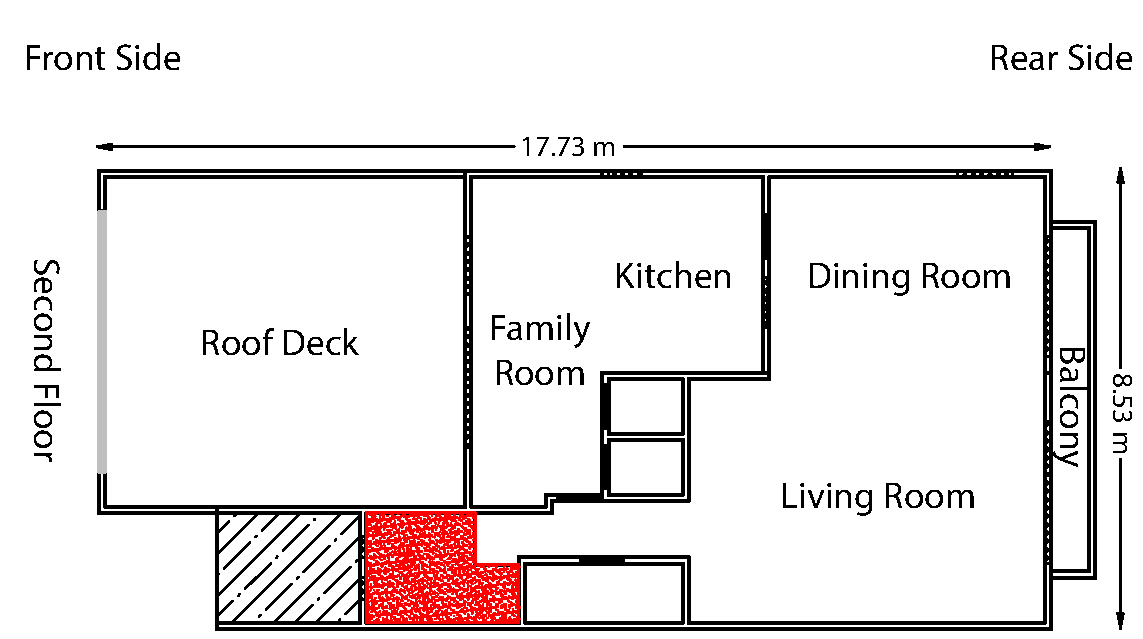
\includegraphics[width=5.0in]{../Figures/Plan_Second_Floor}
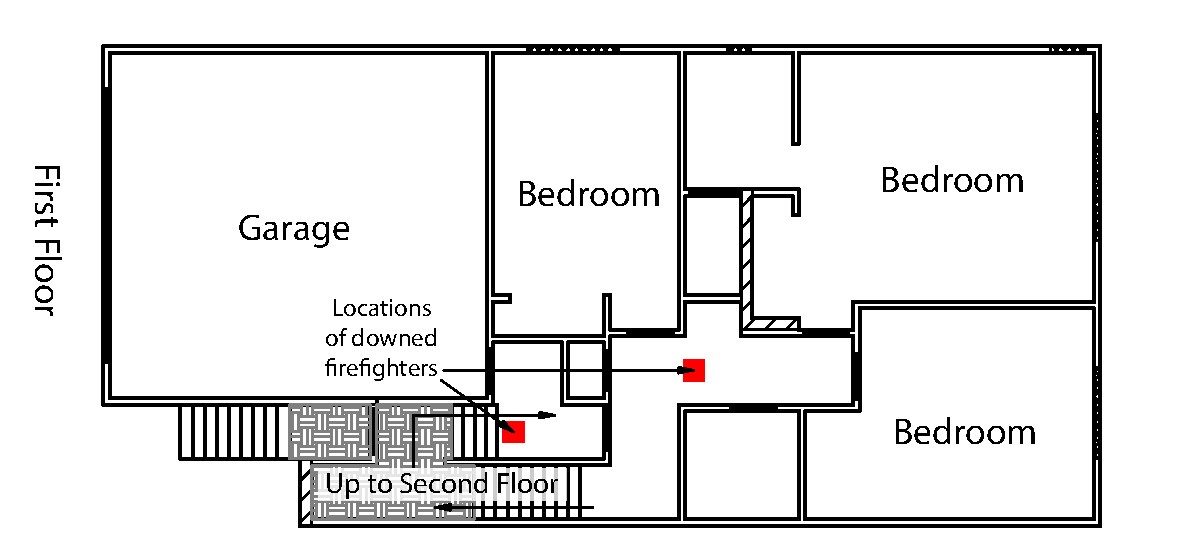
\includegraphics[width=5.0in]{../Figures/Plan_First_Floor}
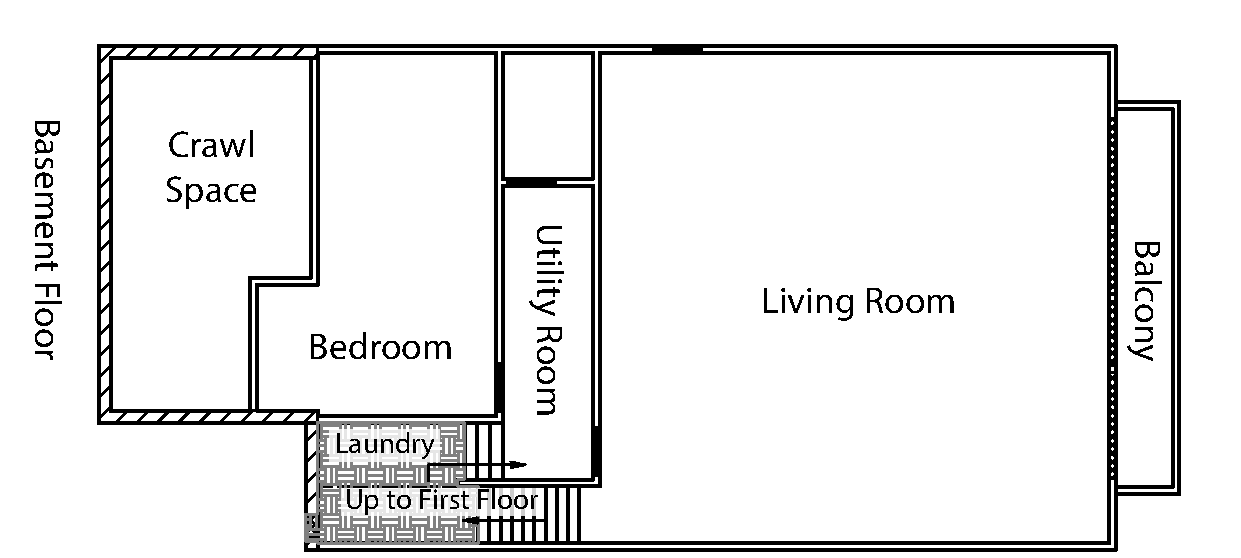
\includegraphics[width=5.0in]{../Figures/Plan_Basement_Floor}
\caption[Plan view of second floor (top), first floor (middle), and basement floor (bottom) of structure.]{Plan view of second floor (top), first floor (middle), and basement floor (bottom) of structure. The fire originated in the living room on the basement floor. Stairs and rooms are identified using information collected by NIST.}
\label{fig:floor_plan}
\end{figure}

\begin{figure}[!ht]
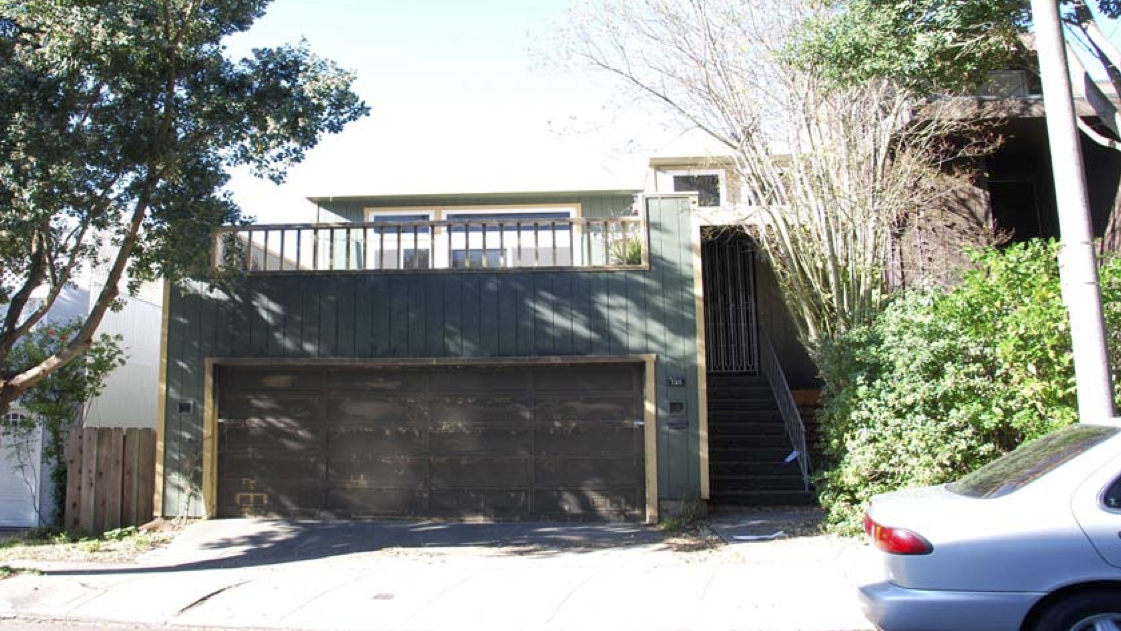
\includegraphics[width=5.50in]{../Figures/Post_Exterior_Front} \\
\vspace{0.1in}
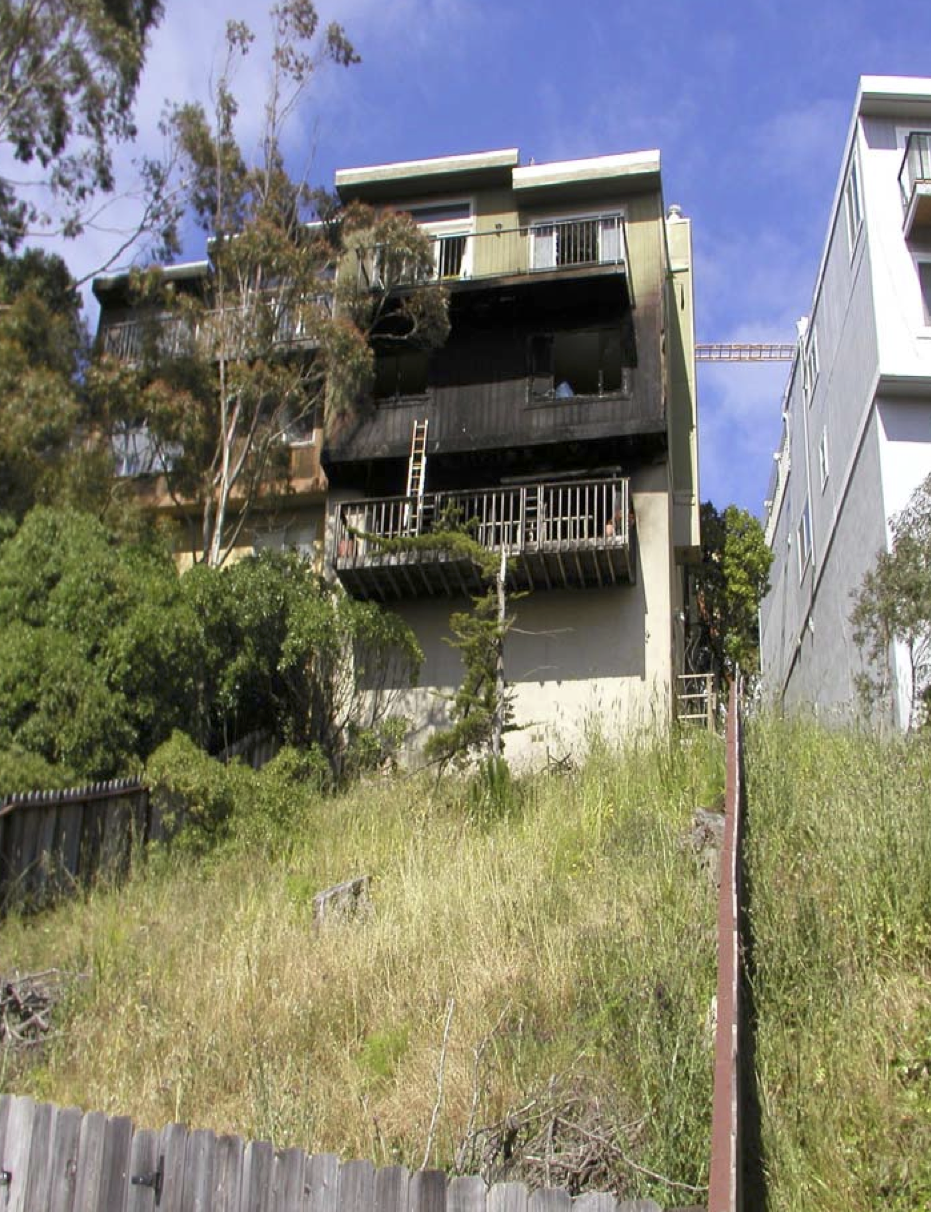
\includegraphics[width=3.50in]{../Figures/Post_Exterior_Rear}
\caption{Front (top) and rear (bottom) exterior of the structure after the incident.}
\label{fig:post_exterior}
\end{figure}

\section{Fires}
\label{sec:fires}

To estimate the type of fuel, fire size, and structure ventilation, on-scene photographs and post-incident reports were used. Based on these sources of information, the FDS model includes three source fires: 1) an initial couch fire in the basement, 2) a flashover fire that involved additional furniture items in the basement, and 3) a fire that occurred on the exterior basement balcony.

The basement primarily contained upholstered polyurethane furniture fuel items, and the balcony was constructed of wood. The HRR of the initial couch fire is based on an experimentally measured HRR for a mattress fire~\cite{madrzykowski2009fire} to represent the fire growth rate of a similar household furniture item. The HRRs of the additional furniture items were estimated based on previous experimental work that characterized the HRR of similar upholstered furniture fuel items~\cite{madrzykowski2009fire,Madrzykowski:2,Babrauskas:1}. Other combustible items and furnishings such as tables, stools, bookshelves, and carpet were present in the basement living room. However, to simplify the analysis and specification of the design fire, only the above fuel items were included because they were considered to have contributed the largest amount of energy in this fire scenario.

The primary fuel packages were located in the basement as shown in Fig.~\ref{fig:fuel_placement}. In this figure, the numbered labels indicate the order in which the fuel items were burning: 1) the initial couch fire, 2) the secondary furniture fuel items, and 3) the balcony fire.

\begin{figure}[!ht]
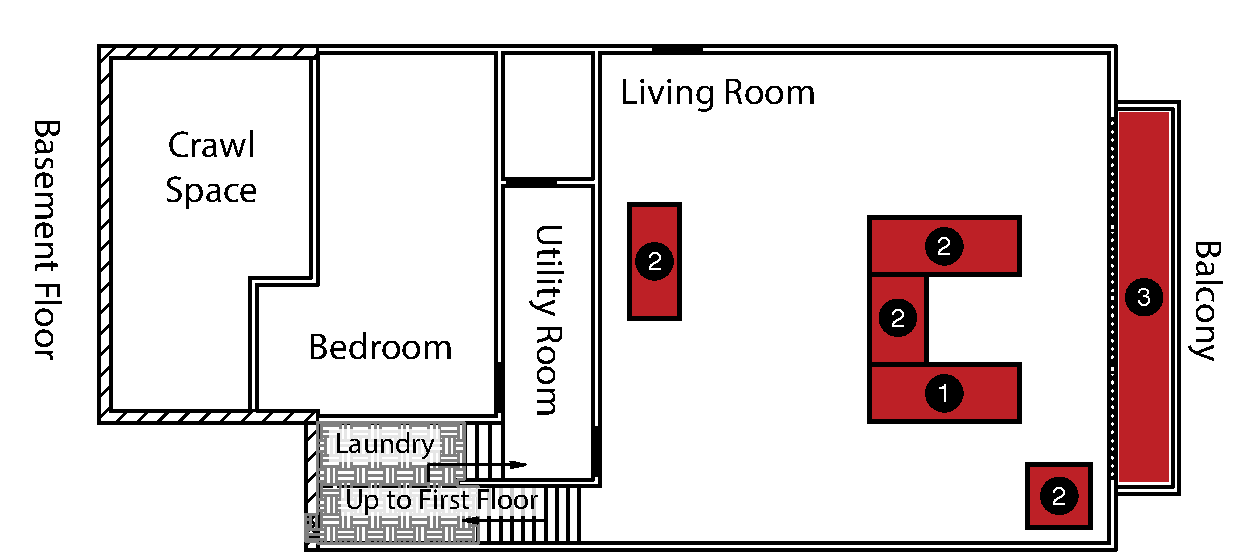
\includegraphics[width=5.5in]{../Figures/Plan_Basement_Fuels}
\caption[Location of fuel items in the basement.]
{Location of fuel items in the basement. The numbered labels indicate the order in which the fuel items were burning: Item~1 is associated with the initial couch fire in the basement, Items~2 are associated with the flashover fire that involved additional furniture items in the basement, and Item~3 is associated with a fire that occurred on the exterior basement balcony.}
\label{fig:fuel_placement}
\end{figure}


\clearpage


Since the time at which the fire started is not known relative to the notification of a fire or how fast the fire spread, several simplifying assumptions were made. One assumption is that the initial couch fire in the basement was specified to start at the beginning of the simulation. The duration of the fire simulation was 9~min (540~s). The beginning of the simulation (0~s) was selected to correspond to an on-scene time of 10:53:00, which was approximately five minutes after the fire department arrived on scene and approximately one minute before the E26 firefighting crew stated that the fire was located below the first floor. The end of the simulation (540~s) was selected to correspond to an on-scene time of 11:02:00, which is the time at which fire suppression operations began (see Table~\ref{tab:incident_timeline}).

The HRRs for the three primary source fires were prescribed in FDS as follows.

\begin{enumerate}
\item For the initial couch fire in the basement, the HRR from 0~s to 327~s followed the experimentally measured mattress HRR~\cite{madrzykowski2009fire}. The HRR at 300~s was approximately 3~MW, and the HRR at 327~s was approximately 5~MW. From 327~s until 540~s (the end of the simulation), the HRR of the initial couch item was specified as a constant 5~MW.

\item The secondary fuel packages in the basement were divided among four additional furniture items (two couches, a lounge, and a chair). The HRRs of these additional furniture items were estimated based on previous experimental work that characterized the HRR of similar upholstered furniture fuel items, which reported HRRs of upholstered chairs and couches ranging from 2~MW to 5~MW~\cite{madrzykowski2009fire,Madrzykowski:2,Babrauskas:1,Janssens:2012}. The two large couches in the middle of the basement were specified with a peak HRR of 5~MW for each item. The lounge and chair located at the perimeter of the basement were specified with a peak HRR of 2~MW for each item. Therefore, the peak HRR of all four furniture items was a total of 14~MW.

Based on post-incident reports and photographs, the HRR of these fuels was specified as follows. From 0~s to 300~s, these items were not burning. From 300~s to 342~s (the time at which the first basement window failed), the secondary fuel items were ignited, and the total HRR of the four furniture items increased linearly from 0~MW to 14~MW. From 342~s to 540~s (the end of the simulation), the total HRR of the four furniture items was specified as a constant 14~MW.

\item The third exterior fuel item included the wood on the basement balcony and siding. To estimate the heat release rate per unit area (HRRPUA) of wood, Babrauskas and Grayson~\cite{babrauskas1990} conducted experiments in a cone calorimeter\footnote{The cone calorimeter is an experimental apparatus used to gather data about the ignition time, mass loss, combustion products, and heat release rate among other properties associated with burning small samples of materials~\cite{ASTM:E1355}.} to determine the 5-min average of the HRRPUA for several different types of wood over a range of radiant heat fluxes. The results of that study indicate that the HRRPUA for different types of wood is approximately 50~kW/m$^2$.

Based on post-incident reports and photographs, the HRR of these fuels was specified as follows. From 0~s to 440~s, the wooden items were not burning. From 440~s to 450~s, the exterior basement balcony was ignited, and the total HRR increased linearly from 0~MW to 1~MW (based on the surface area of the burning wood). From 450~s until 540~s (the end of the simulation), the HRR of the wooden balcony and siding was specified as a constant 5~MW.
\end{enumerate}


\clearpage


Figure~\ref{fig:hrr} shows the overall prescribed design fire for this scenario, which is the sum of the HRRs of the three source fires. In this figure, the text labels indicate the three stages of the fire based on the contribution of the fuel packages. Therefore, the estimated maximum specified fire size for this structure was approximately 20~MW. Note that the prescribed HRR can be different than the simulated HRR calculated by FDS based on the amount of available fuel, oxygen, and ventilation. A comparison of the prescribed HRR and the simulated HRR is discussed in Section~\ref{sec:HRR}.

\begin{figure}[!ht]
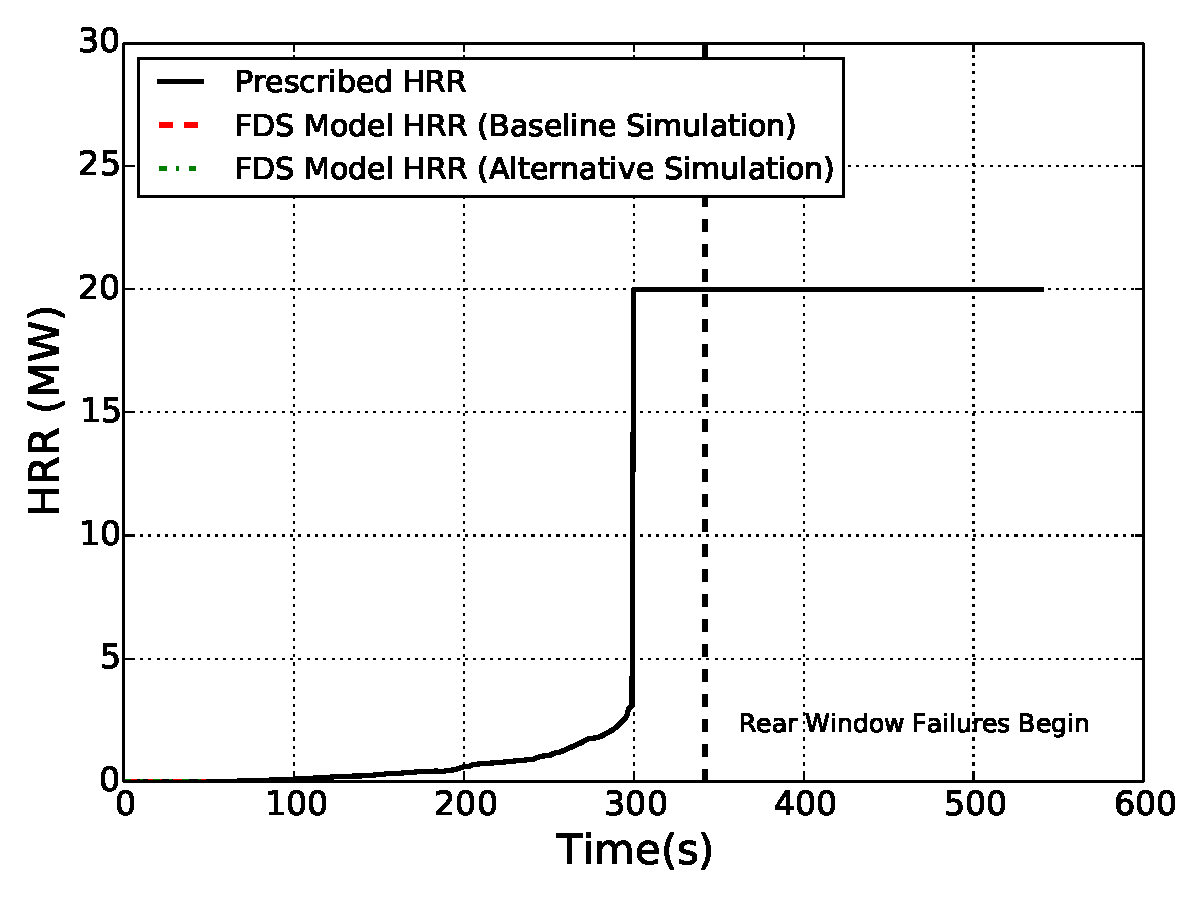
\includegraphics[width=5.5in]{../Figures/Fire_HRR}
\caption[Prescribed HRR vs. time.]
{Prescribed HRR vs. time. The text labels indicate the three stages of the fire based on the contribution of the fuel packages.}
\label{fig:hrr}
\end{figure}

Polyurethane fuel was specified for the interior basement fuel items, which can be represented by the chemical formula, $\C\H_{1.8}\O_{0.30}\N_{0.05}$, with specified product yields of soot ($y_{\mathrm{s}}=0.131 \; \mathrm{kg}/\mathrm{kg}$) and carbon monoxide ($y_{\mathrm{CO}}=0.010 \; \mathrm{kg}/\mathrm{kg}$)~\cite{SFPE:Tewarson}. The product yields are expressed in terms of the amount soot or carbon monoxide emitted per unit mass of fuel consumed~(kg/kg) and can be found in the Society of Fire Protection Engineers (SFPE) Handbook~\cite{SFPE:Tewarson}. A balanced chemical reaction for polyurethane combustion can be written as:

\begin{multline}
\C\H_{1.8}\O_{0.30}\N_{0.05} + 5.22(0.208\,\O_{2} + 0.783\,\N_{2} + 8.34 \times 10^{-3}\,\H_{2}\O + 3.87 \times 10^{-4}\,\C\O_{2}) \\
\rightarrow 6.06(0.129\,\C\O_{2} + 0.156\,\H_{2}\O + 0.001\,\C\O + 0.035\,\C + 0.679\,\N_{2})
\label{eq:fuel_polyurethane}
\end{multline}


\clearpage


Wood fuel was specified for the exterior basement balcony fuel items, which can be represented by the chemical formula, $\C\H_{1.7}\O_{0.74}\N_{0.002}$, with specified product yields of soot ($y_{\mathrm{s}}=0.015 \; \mathrm{kg}/\mathrm{kg}$) and carbon monoxide ($y_{\mathrm{CO}}=0.004 \; \mathrm{kg}/\mathrm{kg}$)~\cite{SFPE:Tewarson}. A balanced chemical reaction for wood combustion can be written as:

\begin{multline}
\C\H_{1.7}\O_{0.74}\N_{0.002} + 4.91(0.208\,\O_{2} + 0.783\,\N_{2} + 8.34 \times 10^{-3}\,\H_{2}\O + 3.87 \times 10^{-4}\,\C\O_{2}) \\
\rightarrow 5.74(0.168\,\C\O_{2} + 0.155\,\H_{2}\O + 6.37 \times 10^{-4}\,\C\O + 5.57 \times 10^{-3}\,\C + 0.670\,\N_{2})
\label{eq:fuel_wood}
\end{multline}

The heat of combustion of polyurethane and wood were specified as 26,200~kJ/kg and 16,400~kJ/kg, respectively, based on data provided in the SFPE Handbook~\cite{SFPE:Tewarson}. The heat of combustion quantifies the amount of energy released per unit mass of the fuel. The following text defines Eqs.~\ref{eq:fuel_polyurethane} and \ref{eq:fuel_wood} for an FDS input file with the two fuels and reaction properties discussed above:

\begin{lstlisting}[basicstyle=\ttfamily\scriptsize]
&SPEC ID = 'POLYURETHANE',    FORMULA = 'CH1.8O0.30N0.05' /
&SPEC ID = 'WOOD',            FORMULA = 'CH1.7O0.74N0.002' /
&SPEC ID = 'OXYGEN',          LUMPED_COMPONENT_ONLY = .TRUE. /
&SPEC ID = 'NITROGEN',        LUMPED_COMPONENT_ONLY = .TRUE. /
&SPEC ID = 'WATER VAPOR',     LUMPED_COMPONENT_ONLY = .TRUE. /
&SPEC ID = 'CARBON MONOXIDE', LUMPED_COMPONENT_ONLY = .TRUE. /
&SPEC ID = 'CARBON DIOXIDE',  LUMPED_COMPONENT_ONLY = .TRUE. /
&SPEC ID = 'SOOT',            LUMPED_COMPONENT_ONLY = .TRUE. /

&SPEC ID = 'AIR',
    SPEC_ID = 'OXYGEN','NITROGEN','WATER VAPOR','CARBON DIOXIDE',
    VOLUME_FRACTION = 0.208057, 0.783214, 0.008342, 0.000387,
    BACKGROUND = .TRUE. /

&SPEC ID = 'PRODUCTS_POLYURETHANE',
    SPEC_ID = 'NITROGEN','WATER VAPOR','CARBON DIOXIDE','CARBON MONOXIDE','SOOT',
    VOLUME_FRACTION = 0.678838, 0.155754, 0.129475, 0.001139, 0.034794 /

&REAC ID = 'POLYURETHANE'
    FUEL = 'POLYURETHANE',
    HEAT_OF_COMBUSTION = 26200,
    SPEC_ID_NU = 'POLYURETHANE','AIR','PRODUCTS_POLYURETHANE'
    NU = -1, -5.218633, 6.057861 /

&SPEC ID = 'PRODUCTS_WOOD',
    SPEC_ID = 'NITROGEN','WATER VAPOR','CARBON DIOXIDE','CARBON MONOXIDE','SOOT',
    VOLUME_FRACTION = 0.670128, 0.155268, 0.168397, 0.000637, 0.005570 /

&REAC ID = 'WOOD'
    FUEL = 'WOOD',
    HEAT_OF_COMBUSTION = 16400,
    SPEC_ID_NU = 'WOOD','AIR','PRODUCTS_WOOD'
    NU = -1, -4.908330, 5.738119 /
\end{lstlisting}

Note that using the input lines above will invoke the simple chemistry reaction mechanism in FDS in which fuel and air react to form only CO$_2$, CO, H$_2$O, soot, and N$_2$. If the inclusion of other combustion products is desired, then the user must explicitly define those species and the chemical reaction that produces them~\cite{FDS_Users_Guide}. Based on the above input lines, FDS uses the default, mixing-controlled fast chemistry combustion model. This mechanism states that the rate of fuel consumption is proportional to both the local limiting reactant concentration and the local rate of mixing and extinction is based on the critical flame temperature approach~\cite{FDS_Math_Guide}. While FDS provides users with the option to use a more complex finite-rate combustion mechanism, there is not sufficient evidence in this case to justify deviating from the default specifications.

Another simplification of the model is that the sources of the gas phase polyurethane and wood fuel have constant areas at fixed locations (five furniture items in the basement interior for the polyurethane fuel, and the exterior basement balcony for the wood fuel).

A time-dependent burning rate was specified for each of the fuel packages in terms of a fuel mass flux. The fuel mass flux is the amount of fuel vapor per unit area that is released from the surface of each fuel package shown in Fig.~\ref{fig:fuel_placement}. The specified time-dependent fuel mass flux for each fuel package corresponds to the HRRs that were described earlier. The HRR from each individual fuel package contributes to the total HRR shown in Fig.~\ref{fig:hrr}. FDS then determines the amount of combustion that occurs throughout the simulation based on the amount of available fuel and oxygen at a given location. The following lines define the fire surfaces for each fuel package in the FDS input file:

\begin{lstlisting}
&SURF ID='COUCH_RIGHT_INITIAL',
    SPEC_ID='POLYURETHANE',
    MASS_FLUX = 5.271815E-6,
    RAMP_MF='COUCH_RIGHT_INITIAL_RAMP' /

&SURF ID='COUCH_MIDDLE_FLASHOVER',
    SPEC_ID='POLYURETHANE',
    MASS_FLUX = 1.037172E-5,
    RAMP_MF='COUCH_MIDDLE_FLASHOVER_RAMP' /

&SURF ID='COUCH_LEFT_FLASHOVER',
    SPEC_ID='POLYURETHANE',
    MASS_FLUX = 5.271815E-6,
    RAMP_MF='COUCH_LEFT_FLASHOVER_RAMP' /

&SURF ID='LOUNGE_FLASHOVER',
    SPEC_ID='POLYURETHANE',
    MASS_FLUX = 7.853485E-6,
    RAMP_MF='LOUNGE_FLASHOVER_RAMP' /

&SURF ID='CHAIR_FLASHOVER',
    SPEC_ID='POLYURETHANE',
    MASS_FLUX = 7.918660E-6,
    RAMP_MF='CHAIR_FLASHOVER_RAMP' /

&SURF ID='WOOD_EXTERIOR',
    SPEC_ID='WOOD',
    MASS_FLUX = 0.003049,
    RAMP_MF='WOOD_EXTERIOR_RAMP' /
\end{lstlisting}

Note that the mass flux values here are unique for each fuel item and are specific to the input files used for these simulations. The key point is that each fuel item was modeled as a 3D object with flat surfaces from which a specified amount of fuel flows, mixes with air, and burns.


\clearpage


\section{Materials}
\label{sec:materials}

While the fires were represented as fuel sources with a constant area (Section~\ref{sec:fires}), from a heat transfer perspective, it is important to define the material properties (density, thermal conductivity, specific heat, and thickness) to account for heat transfer and energy storage in the ceiling, walls, and floor. In this study, the material properties of gypsum board~\cite{WAKILI2007} were specified on the finished walls and ceilings of the structure. The following lines define the gypsum material and surface properties in the FDS input file:

\begin{lstlisting}
&MATL ID          = 'GYPSUM'
    FYI           = 'Wakili - Journal of Fire Sciences 2007' 
    CONDUCTIVITY  = 0.28
    SPECIFIC_HEAT = 1.00
    DENSITY       = 810. /

&SURF ID      = 'WALL'
    DEFAULT   = .TRUE.
    COLOR     = 'DARK SEA GREEN 4'
    MATL_ID   = 'GYPSUM'
    THICKNESS = 0.012 /
\end{lstlisting}

\section{Ventilation}
\label{sec:ventilation}

The simulations in this study account for changes in the ventilation due to a combination of fire department operations (opening doors) and fire acting on the structure (fire breaching walls, breaking windows, etc). The ventilation times and ventilation areas represent our best understanding of the incident. The times of ventilation changes for doors and windows are provided in Table~\ref{tab:ventilation_timeline}.

During the time at which the downed firefighters were located, the state of some windows and doors in the structure was known, which resulted in the establishment of a flow path in the interior stairwell leading into the basement. However, the exact time of operation for other doors was not known. Therefore, the following doors were assumed to be open at the start of the simulation: 1) the front door, 2) the interior door leading from the hallway on the first floor into the stairwell towards the basement, 3) the door leading from the garage into the first floor landing, and 4) the overhead garage door. The basement windows and exterior door were specified to open at certain times based on observations of failure (i.e., window breakage) or fire department operations (i.e., forcible entry) from on-scene photographs and post-incident reports.

Structure leakage has been shown to be important when modeling enclosure fires~\cite{beal2009}. The open front door at the start of the simulation and the vents created during the simulation are significantly larger than the total effective area of leakage of a structure of this type. Therefore, any leakage in the structure would have a negligible impact on the fluid mechanics within the structure and is not included in this study.

\begin{table}[!ht]
\caption[Timeline of ventilation events in the simulation]{Timeline of ventilation events in the simulation}
\begin{tabular}{ccll}
\toprule
Simulation Time      &  Ventilation Area  &  Ventilation Type    &  Ventilation Location     \\
{(s)}                &  (m$^2$)           &                      &                           \\
\midrule
0                    &  1.47              &  Door                &  Front Entry Exterior     \\
0                    &  10.1              &  Overhead Door       &  Front Garage Exterior    \\
0                    &  1.68              &  Door                &  Stairwell Interior       \\
0                    &  1.68              &  Door                &  Garage Interior          \\
342                  &  1.89              &  Sliding Glass Door  &  Rear Basement Exterior   \\
383                  &  1.89              &  Sliding Glass Door  &  Rear Basement Exterior   \\
383                  &  1.68              &  Door                &  Left Basement Exterior   \\
418                  &  2.52              &  Window              &  Rear Basement Exterior   \\
440                  &  2.31              &  Window              &  Rear Basement Exterior   \\
450                  &  3.78              &  Sliding Glass Door  &  Rear Basement Exterior   \\
\bottomrule
\end{tabular}
\label{tab:ventilation_timeline}
\end{table}

\section{Numerical Mesh}
\label{sec:numerical_mesh}

For the simulation, a measure of how well the flow field is resolved can be estimated by using the non-dimensional expression $D^*/\dx$. Here, $D^*$ is the characteristic fire diameter, $\dx$ is the nominal size of a mesh cell, and $\dQ$ is the total heat release rate of the fire:
\begin{equation}
D^* = \left(
     \frac{\dQ}{\rho_\infty \, c_p \, T_\infty \, \sqrt{g}}
     \right)^\frac{2}{5} 
\label{eq:mesh}
\end{equation}
From the FDS User's Guide~\cite{FDS_Users_Guide}, the characteristic fire diameter is related to the characteristic fire size via the relation $Q^* = (D^*/D)^{5/2}$. Here, $D$ is the physical diameter of the base of the fire specified in the simulation. Based on validation work performed for the U.S. Nuclear Regulatory Commission, $D^*/\dx$ values ranged between 4 and 16~\cite{NUREG_1824} and produced results that were adequate for engineering calculations. Following Eq.~\ref{eq:mesh} and using a grid cell size of 10~cm, the ratio of the characteristic fire diameter to cell size ($D^*/\dx$) was 18 for the initial couch fire (combined HRR of 5~MW), 31 for the secondary flashover fire in the basement (combined HRR of 19~MW), and 32 for the maximum prescribed fire size in the structure (combined HRR of 20~MW). Therefore, the grid resolution used in this model results in a $D^*/\dx$ ratio that exceeds typical engineering values.

As discussed in Section~\ref{sec:geometry}, the structure had exterior dimensions of 8.53~m (28~ft) by 17.73~m (58~ft) and a total height of 5.9~m (19~ft). To ensure adequately resolved fluid flow in and out of the structure, the computational domain was extended beyond the volume of the structure. The dimensions of the computational domain were 11.5~m (38~ft) by 22~m (72~ft) and a height of 13.6~m (45~ft). A grid resolution of 10~cm (3.9~in) was used, which resulted in a total of approximately 3.4 million computational cells. As a result, all of the input model geometry lengths, ventilation openings (holes, doors, and windows), and fire areas will snap to the nearest 10~cm. Figure~\ref{fig:SMV_exterior_grid} shows the front and rear sides of the structure rendered in Smokeview with the 10~cm mesh.

\begin{figure}[!ht]
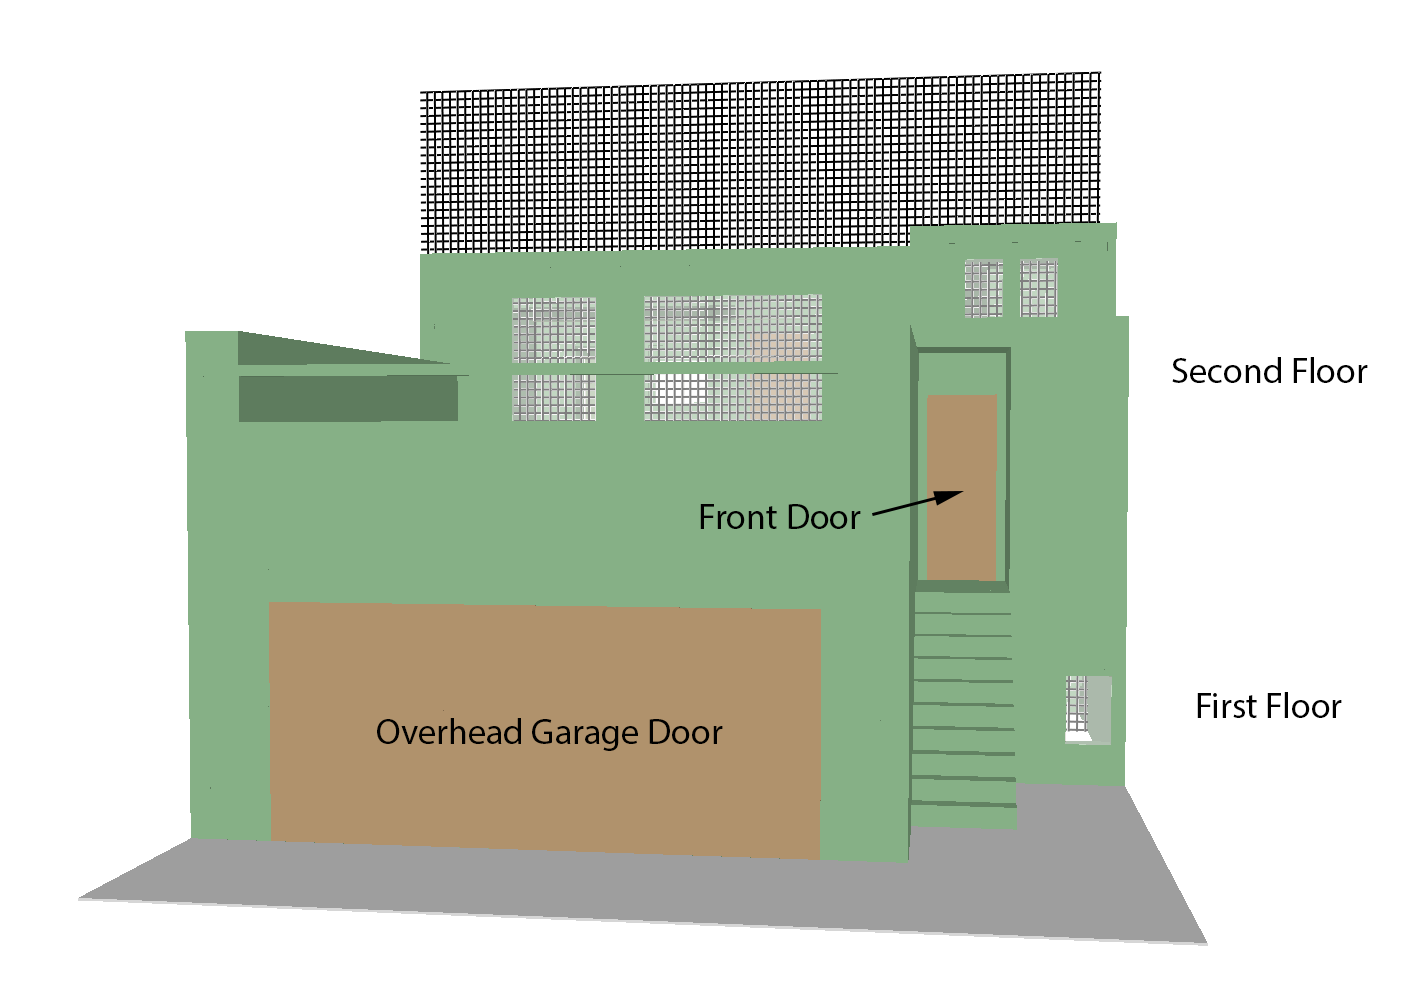
\includegraphics[width=5.0in]{../Figures/SMV_Exterior_Grid_Front} \\
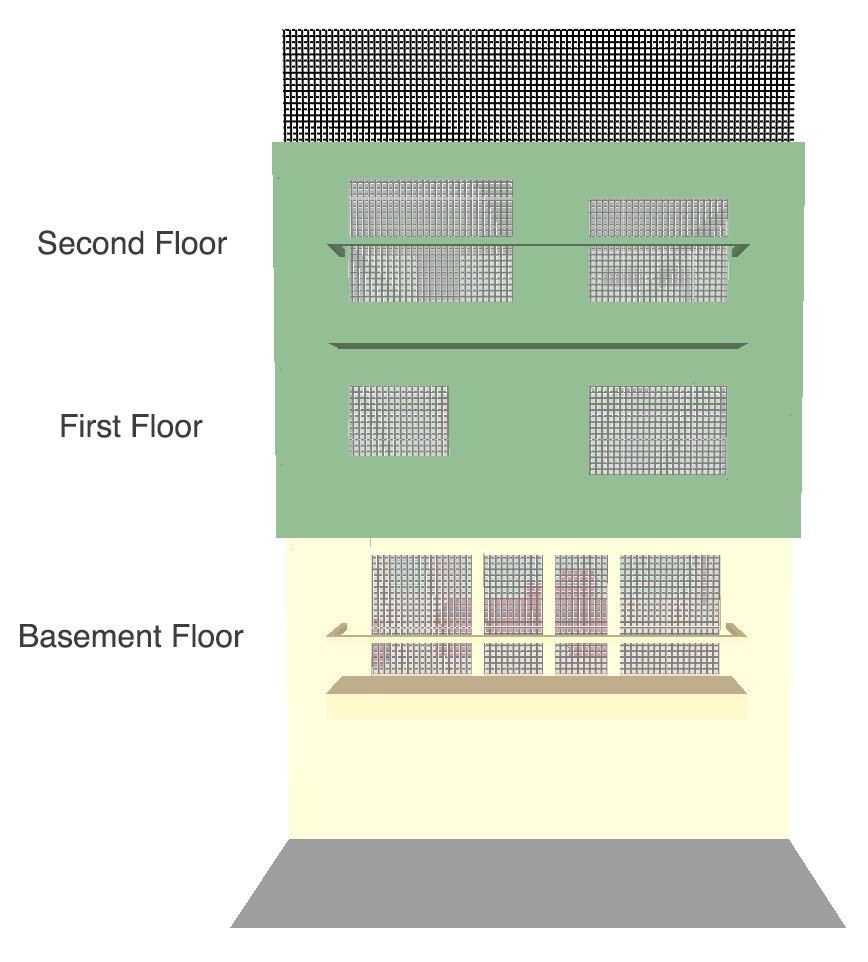
\includegraphics[width=4.5in]{../Figures/SMV_Exterior_Grid_Rear}
\caption{Front (top) and rear (bottom) of the structure with a 10~cm computational mesh.}
\label{fig:SMV_exterior_grid}
\end{figure}


\clearpage


The domain was divided into 16 meshes (each containing between 184,000 and 248,200 grid cells) that could be processed in parallel, which reduced the amount of required calculation time to approximately 2~days. Figure~\ref{fig:mult_mesh} shows the entire structure within the computational domain that has been divided into multiple meshes. Table~\ref{tab:model_parameters} shows a summary of the model input parameters for the simulations that were conducted as part of this study.

\begin{figure}[!ht]
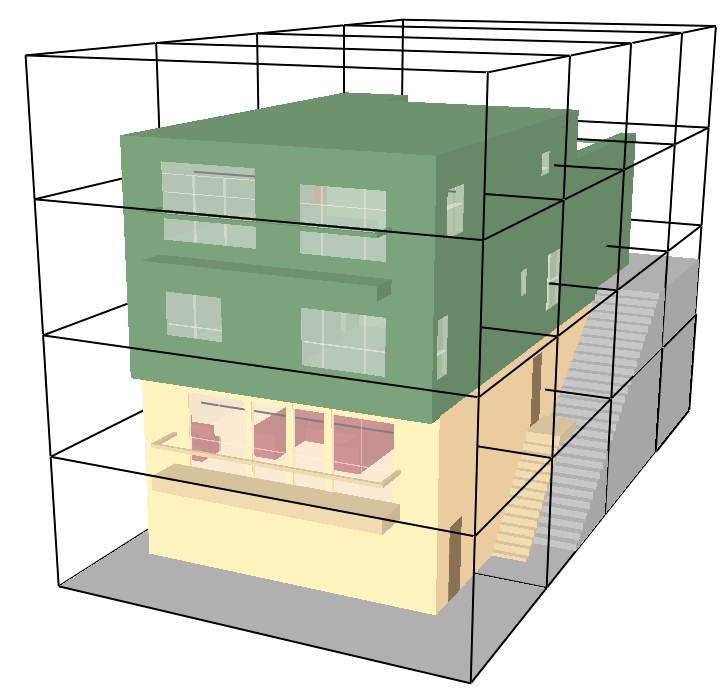
\includegraphics[width=4.5in]{../Figures/SMV_Exterior_Meshes}
\caption[Rear-left side of the structure within the computational domain.]
{Rear-left side of the structure within the computational domain with multiple meshes.}
\label{fig:mult_mesh}
\end{figure}

\begin{table}[!ht]
\caption[Relevant fire model input parameters]{Relevant fire model input parameters}
\begin{tabular}{lll}
\toprule
Parameter                                    &  Description                                  &  Discussion                        \\
\midrule
Simulation Time                              &  9~min                                        &  --                                \\
Grid Cell Size                               &  10~cm                                        &  Section~\ref{sec:numerical_mesh}  \\
Ambient Temperature$^*$                      &  20~$^{\circ}$C (68~$^{\circ}$F)              &  --                                \\
Reaction: Polyurethane~\cite{SFPE:Tewarson}  &  Formula: $\C\H_{1.8}\O_{0.30}\N_{0.05}$      &  Section~\ref{sec:fires}           \\
                                             &  Soot Yield: 0.131~$\mathrm{kg}/\mathrm{kg}$  &                                    \\
                                             &  CO Yield: 0.010~$\mathrm{kg}/\mathrm{kg}$    &                                    \\
                                             &  Heat of combustion: 26,200~kJ/kg             &                                    \\
Reaction: Wood~\cite{SFPE:Tewarson}          &  Formula: $\C\H_{1.7}\O_{0.74}\N_{0.002}$     &  Section~\ref{sec:fires}           \\
                                             &  Soot Yield: 0.015~$\mathrm{kg}/\mathrm{kg}$  &                                    \\
                                             &  CO Yield: 0.004~$\mathrm{kg}/\mathrm{kg}$    &                                    \\
                                             &  Heat of combustion: 16,400~kJ/kg             &                                    \\
Peak HRRs                                    &  Initial couch fire: 5~MW                     &  Section~\ref{sec:fires}           \\
                                             &  Basement flashover fire: 14~MW               &                                    \\
                                             &  Basement balcony fire: 1~MW                  &                                    \\
Material: Gypsum Board~\cite{WAKILI2007}     &  Thermal conductivity: 0.28~\si{W/(m.K)}      &  Section~\ref{sec:materials}       \\
                                             &  Density: 810~kg/m$^3$                        &                                    \\
                                             &  Specific heat: 1.0~\si{kJ/(kg.K)}            &                                    \\
                                             &  Thickness: 1.2~\si{cm}                       &                                    \\
\bottomrule
\end{tabular}
\footnotesize
\\ $^{*}$Initial interior temperature was assumed to be 20~$^{\circ}$C; actual exterior temperature was 14~$^{\circ}$C~\cite{NIOSH:Bowyer2}.
\normalsize
\label{tab:model_parameters}
\end{table}


\chapter{Model Results}
\label{sec:model_results}

To examine the results of the simulations, it is important to link the timelines from the fire scene to the simulation times. Table~\ref{tab:combined_timeline} shows the fireground timeline~\cite{NIOSH:Bowyer2} along with the corresponding simulation times.

\begin{table}[!ht]
\caption[Fire incident and simulation event timeline]{Fire incident and simulation event timeline}
\begin{tabular}{ccl}
\toprule
Incident Time  &  Simulation  &  Fire Behavior / Fireground Operation                                \\
               &  Time        &                                                                      \\
{(hh:mm:ss)}   &  {(s)}       &                                                                      \\
\midrule
10:45:00       &              &  Dispatch for a curtain fire due to an electrical short at a         \\
               &              &  residential structure.                                              \\
               &              &                                                                      \\
10:48:00       &              &  E26 arrives on scene, reports light smoke conditions, and           \\
               &              &  makes entry into the front door with a 1~\sfrac{3}{4}~in hoseline.  \\
               &              &                                                                      \\
10:53:00       &  0           &  FDS simulation begins.                                              \\
               &              &                                                                      \\
10:54:00       &  60          &  E26 crew states that the fire is located below the first floor.     \\
               &              &                                                                      \\
10:56:00       &  180         &  BC9 observes smoke but no fire at the left rear corner              \\
               &              &  of the structure.                                                   \\
               &              &                                                                      \\
10:58:42       &  342         &  Fire self-vents from the rear side of the structure when a glass    \\
               &              &  window in the basement fails. Additional glass windows on the       \\
               &              &  rear side of the structure fail within the next two minutes.        \\
               &              &                                                                      \\
10:59:23       &  383         &  BC9 forces open the basement door on the left side of               \\
               &              &  the structure, reports heavy fire and smoke, and requests a         \\
               &              &  second hoseline.                                                    \\
               &              &                                                                      \\
11:00:00       &  420         &  BC6 notices a severe change in conditions (heavy black smoke        \\
               &              &  from garage).                                                       \\
               &              &                                                                      \\
11:01:00       &  480         &  Heavy fire and black smoke observed at rear of structure.           \\
               &              &  Incident command (IC) attempts to contact E26 several times         \\
               &              &  via radio with no reply.                                            \\
               &              &                                                                      \\
11:02:00       &  540         &  E32 crew makes entry into the basement with a second hoseline       \\
               &              &  and begins suppression operations. FDS simulation ends.             \\
               &              &                                                                      \\
11:08:00       &              &  Two downed E26 firefighters are found on the first floor.           \\
               &              &                                                                      \\
11:09:00       &              &  The downed E26 firefighters are carried out of the structure.       \\
               &              &                                                                      \\
\bottomrule
\end{tabular}
\footnotesize
\\ For specific information regarding ventilation areas used in the FDS model, refer to Table~\ref{tab:ventilation_timeline}.
\normalsize
\label{tab:combined_timeline}
\end{table}


\clearpage


\section{Heat Release Rate}
\label{sec:HRR}

In an FDS simulation, a prescribed HRR is specified, which results in a specified amount of fuel vapor (or pyrolyzate) being released from a fuel surface. FDS then determines the amount of combustion that occurs throughout the simulation based on the amount of available fuel and oxygen at a given location. As a result, the actual HRR in FDS can be different than the prescribed HRR based on the ventilation conditions.

Figure~\ref{fig:hrr_w_fds} shows the HRR vs. time based on the fires that were described in Section~\ref{sec:fires}. The vertical dashed line represents the time at which the first basement window on the rear side of the structure failed (342~s). Additional windows on the rear side of the basement continued to fail within the next two minutes. The maximum size of the fire used in this study was selected such that the conditions would become ventilation limited to minimize computational time while aligning with observations from the actual fire scenario. Note that the rear window failures were manually specified in accordance with the event timeline rather than failure temperature criteria.

\begin{figure}[!ht]
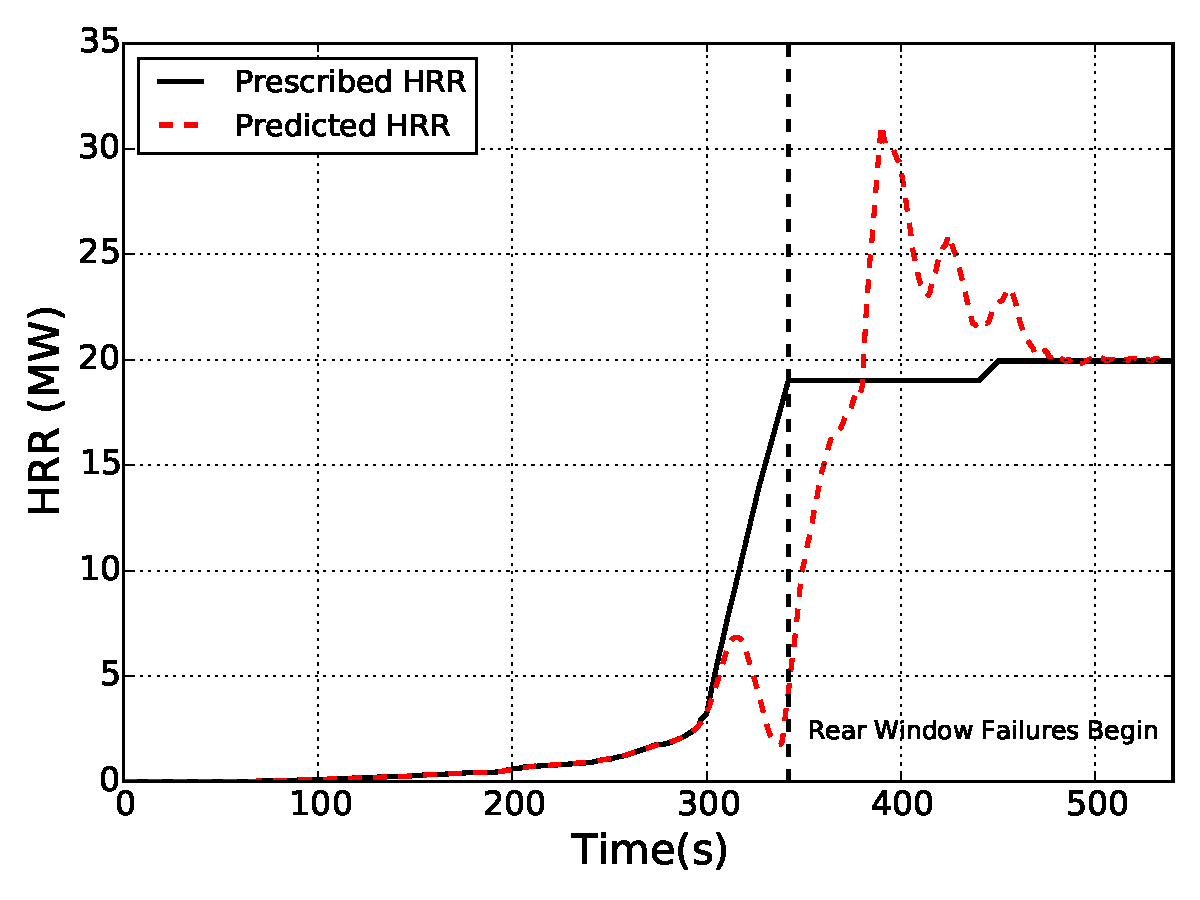
\includegraphics[width=5.5in]{../Figures/Fire_HRR_w_FDS}
\caption[HRR vs. time from the FDS simulations.]
{HRR vs. time from the FDS simulations. The vertical line indicates the time at which the rear basement windows began to fail (342~s).}
\label{fig:hrr_w_fds}
\end{figure}


\clearpage


In Fig.~\ref{fig:hrr_w_fds}, the solid line represents the HRR that was prescribed in the FDS simulation, and the dashed line represents the actual HRR that was predicted by FDS based on the ventilation conditions. From 0~s to 300~s, the predicted HRR was in agreement with the prescribed HRR because there was an adequate amount of oxygen for all of the fuel to combust. From 300~s to 342~s (the time at which the first basement window failed), the predicted HRR was lower than the prescribed HRR because the fire conditions in the structure became ventilation limited. The maximum predicted HRR was approximately 7~MW before the fire conditions became ventilation limited and started to decay. The HRR decreased to approximately 2~MW as the amount of oxygen inside the structure became limited. At this time, there was an insufficient amount of oxygen in the structure to burn all of the fuel; therefore, localized burning occurred near the ventilation openings where ambient air was available.

At a time of 342~s, the first window on the rear side of the structure failed, and additional windows failed within the next two minutes. As additional window failures occurred (see Table~\ref{tab:ventilation_timeline}), the abrupt change in ventilation caused the HRR to increase to approximately 32~MW before it reached a steady-state value of approximately 20~MW. The predicted HRR increased above the prescribed HRR because the unburned fuel and smoke that accumulated in the structure during ventilation-limited conditions was mixing with ambient air from the failed window openings and burning.

Note that the HRR in the simulation might be overpredicted due to limitations in the combustion model related to the reignition of fuel-rich gases. In other words, there is some combustion occurring in the simulation near the front door and second floor as the fuel-rich gases mix with fresh air and reignite, which is not consistent with on-scene and post-incident photographs. However, for the high-hazard areas that are the focus of this study (the basement and interior stairwell), the pressures, temperatures, and velocities are representative of the hazardous flow path conditions that would have occurred in this fire incident.

Figure~\ref{fig:timeline_comparison_rear} shows a time series comparison of on-scene photographs and Smokeview snapshots of flaming combustion that occurred through the failed windows on the rear side of the structure. In this figure, the first photograph is shown at a simulation time of 321~s (approximately 20~s before the first rear basement window failed), the second photograph is shown at a simulation time of 349~s (approximately 10~s after the first rear basement window failed), the third photograph is shown at a simulation time of 440~s (approximately when the third rear basement window failed), and the fourth photograph is shown at a simulation time of 450~s (approximately when all of the rear basement windows failed). Figure~\ref{fig:timeline_comparison_front} shows a comparison of an on-scene photograph and Smokeview snapshot of smoke coming out of the front side of the structure at approximately the time when the rear windows began to fail.

\begin{figure}[!ht]
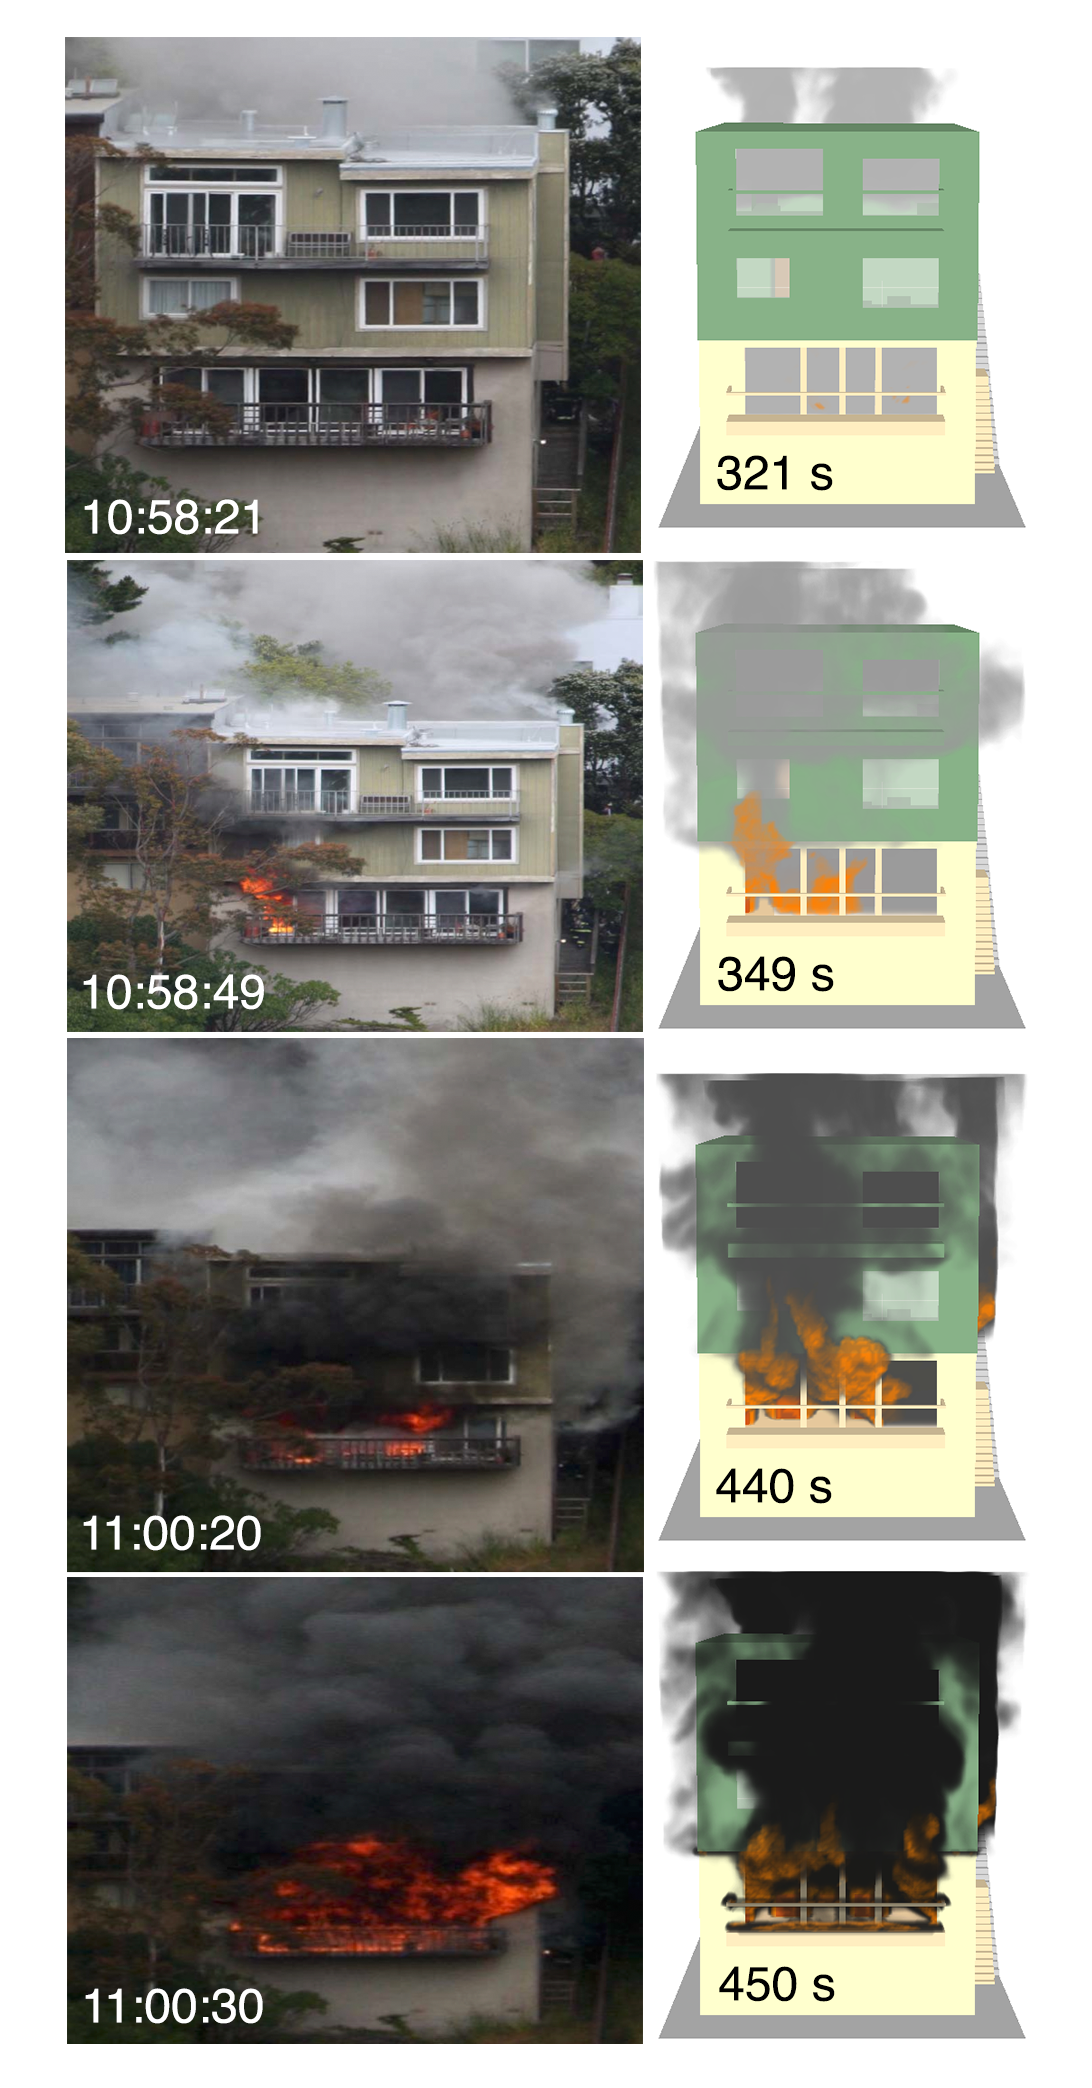
\includegraphics[height=8.0in]{../Figures/Timeline_Comparison}
\caption{Comparison of on-scene photographs and Smokeview snapshots of exterior combustion occurring on the rear side of the structure. The on-scene time is indicated on the left photograph, and the corresponding simulation time is indicated on the right Smokeview snapshot. For more information on the fire incident and simulation timeline, refer to Table~\ref{tab:combined_timeline}.}
\label{fig:timeline_comparison_rear}
\end{figure}

\begin{figure}[!ht]
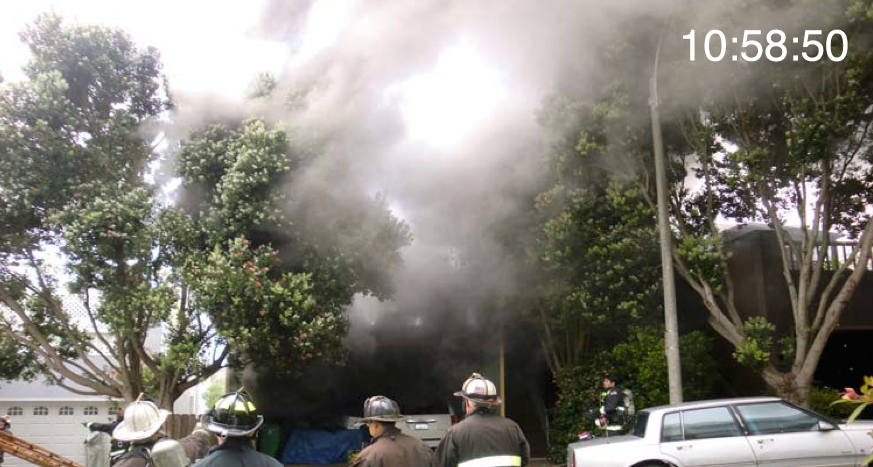
\includegraphics[width=5.0in]{../Figures/Photo_Front_350_s}
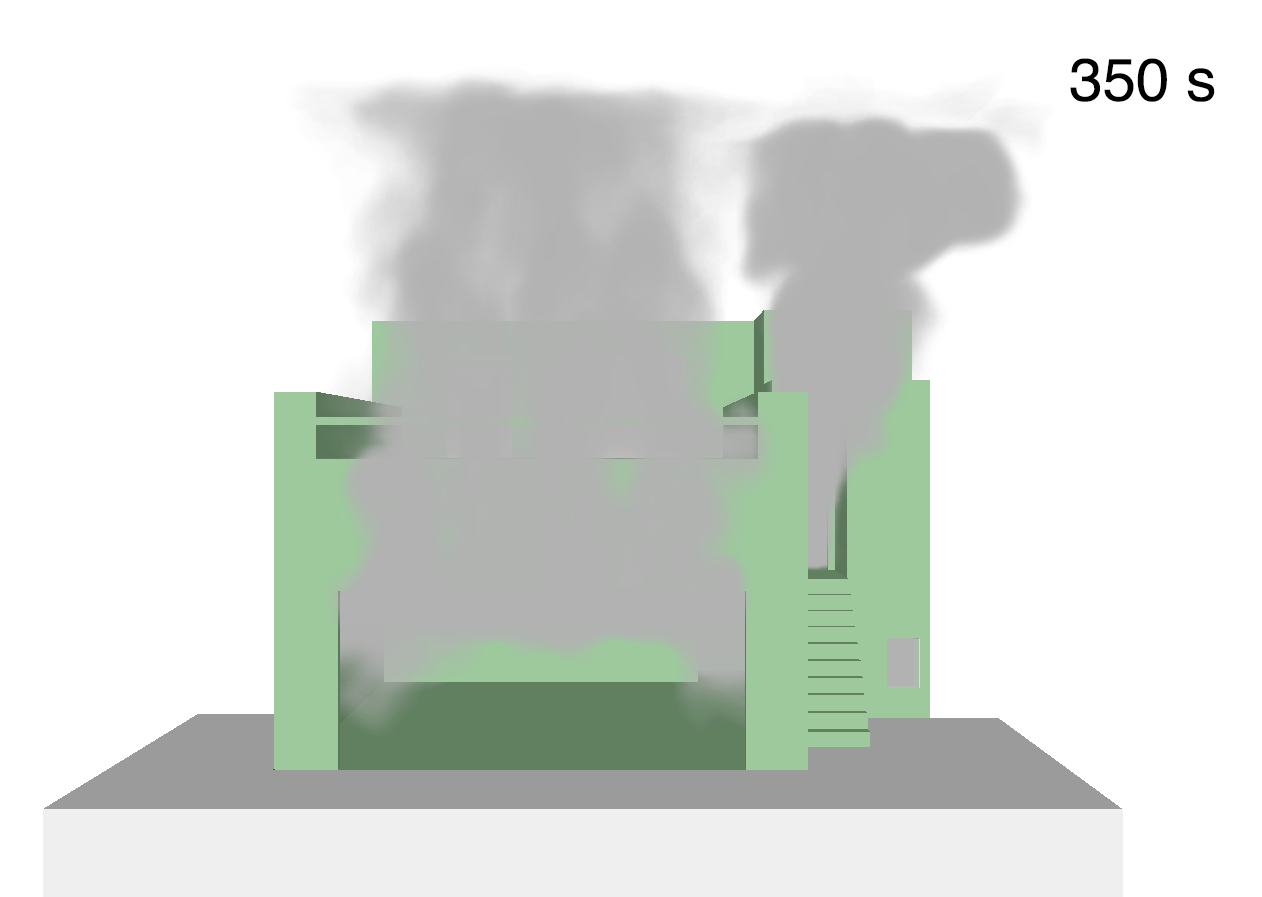
\includegraphics[width=5.0in]{../Figures/SMV_Front_350_s}
\caption{Comparison of an on-scene photograph and Smokeview snapshot of smoke coming out of the front side of the structure. The on-scene time is indicated on the photograph (top), and the corresponding simulation time is indicated on the Smokeview snapshot (bottom). For more information on the fire incident and simulation timeline, refer to Table~\ref{tab:combined_timeline}.}
\label{fig:timeline_comparison_front}
\end{figure}


\clearpage


\section{Pressure}
\label{sec:pressure}

As the simulated fire grew in the basement, the pressure in the basement increased and caused the hot gases to flow upwards from a region of high pressure in the basement to a region low pressure via the interior stairwell. Figure~\ref{fig:smv_pressure} shows the calculated pressure conditions in the structure just before and after the rear basement window failed in the simulation.

In this figure, the pressure profile within the high hazard areas is shown via two snapshots in time to illustrate the change in the interior conditions. The first snapshot is shown at a time of 340~s into the simulation, which is 2~s before the first rear basement window failed, and the second snapshot is shown at a time of 402~s into the simulation, which is 60~s after the first rear basement window failed. The pressure rise in the basement ranges from a 5~Pa ($7.3 \times 10^{-4}$~psi) over-pressure at mid-level height to greater than 10~Pa ($1.5 \times 10^{-3}$~psi) at the ceiling.

\begin{figure}[!ht]
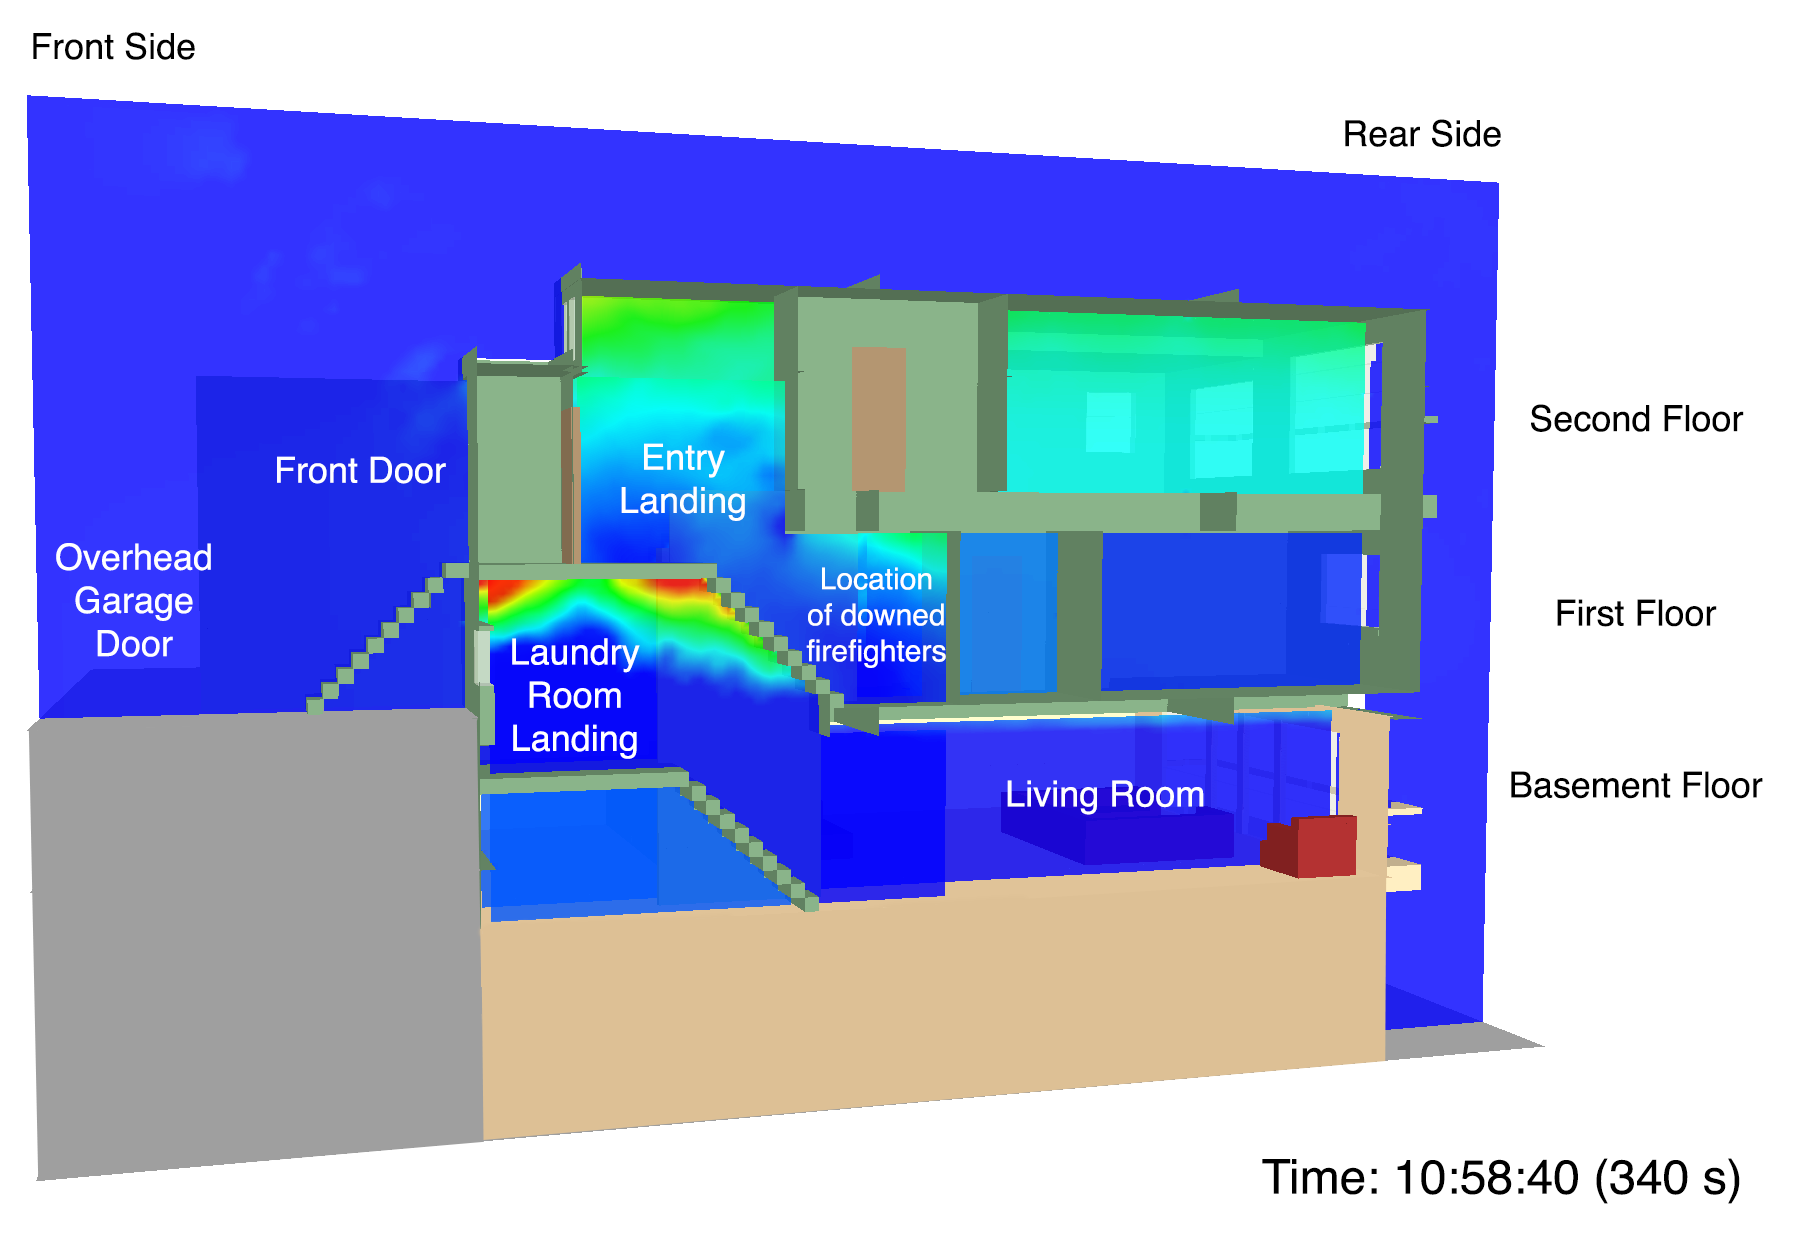
\includegraphics[width=5.5in]{../Figures/SMV_Pres_340_s}
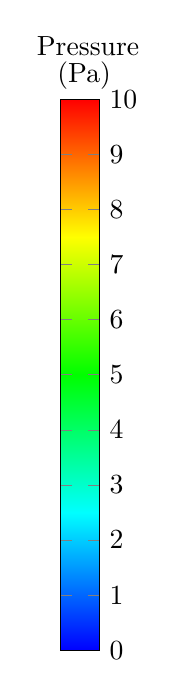
\begin{tikzpicture}
\pgfkeys{/pgf/number format/set thousands separator = {}}
\node at (0.65,0.67) {Pressure};
\node at (0.6,0.3) {(Pa)};
\begin{axis}[
    hide axis,
    scale only axis,
    height=0pt,
    width=0pt,
    colorbar,
    point meta min=0,
    point meta max=10,
    colorbar style={
        height=7cm,
        ytick={0,1,2,...,10}}
    ]
    \addplot [draw=none] coordinates {(0,0)};
\end{axis}
\end{tikzpicture}

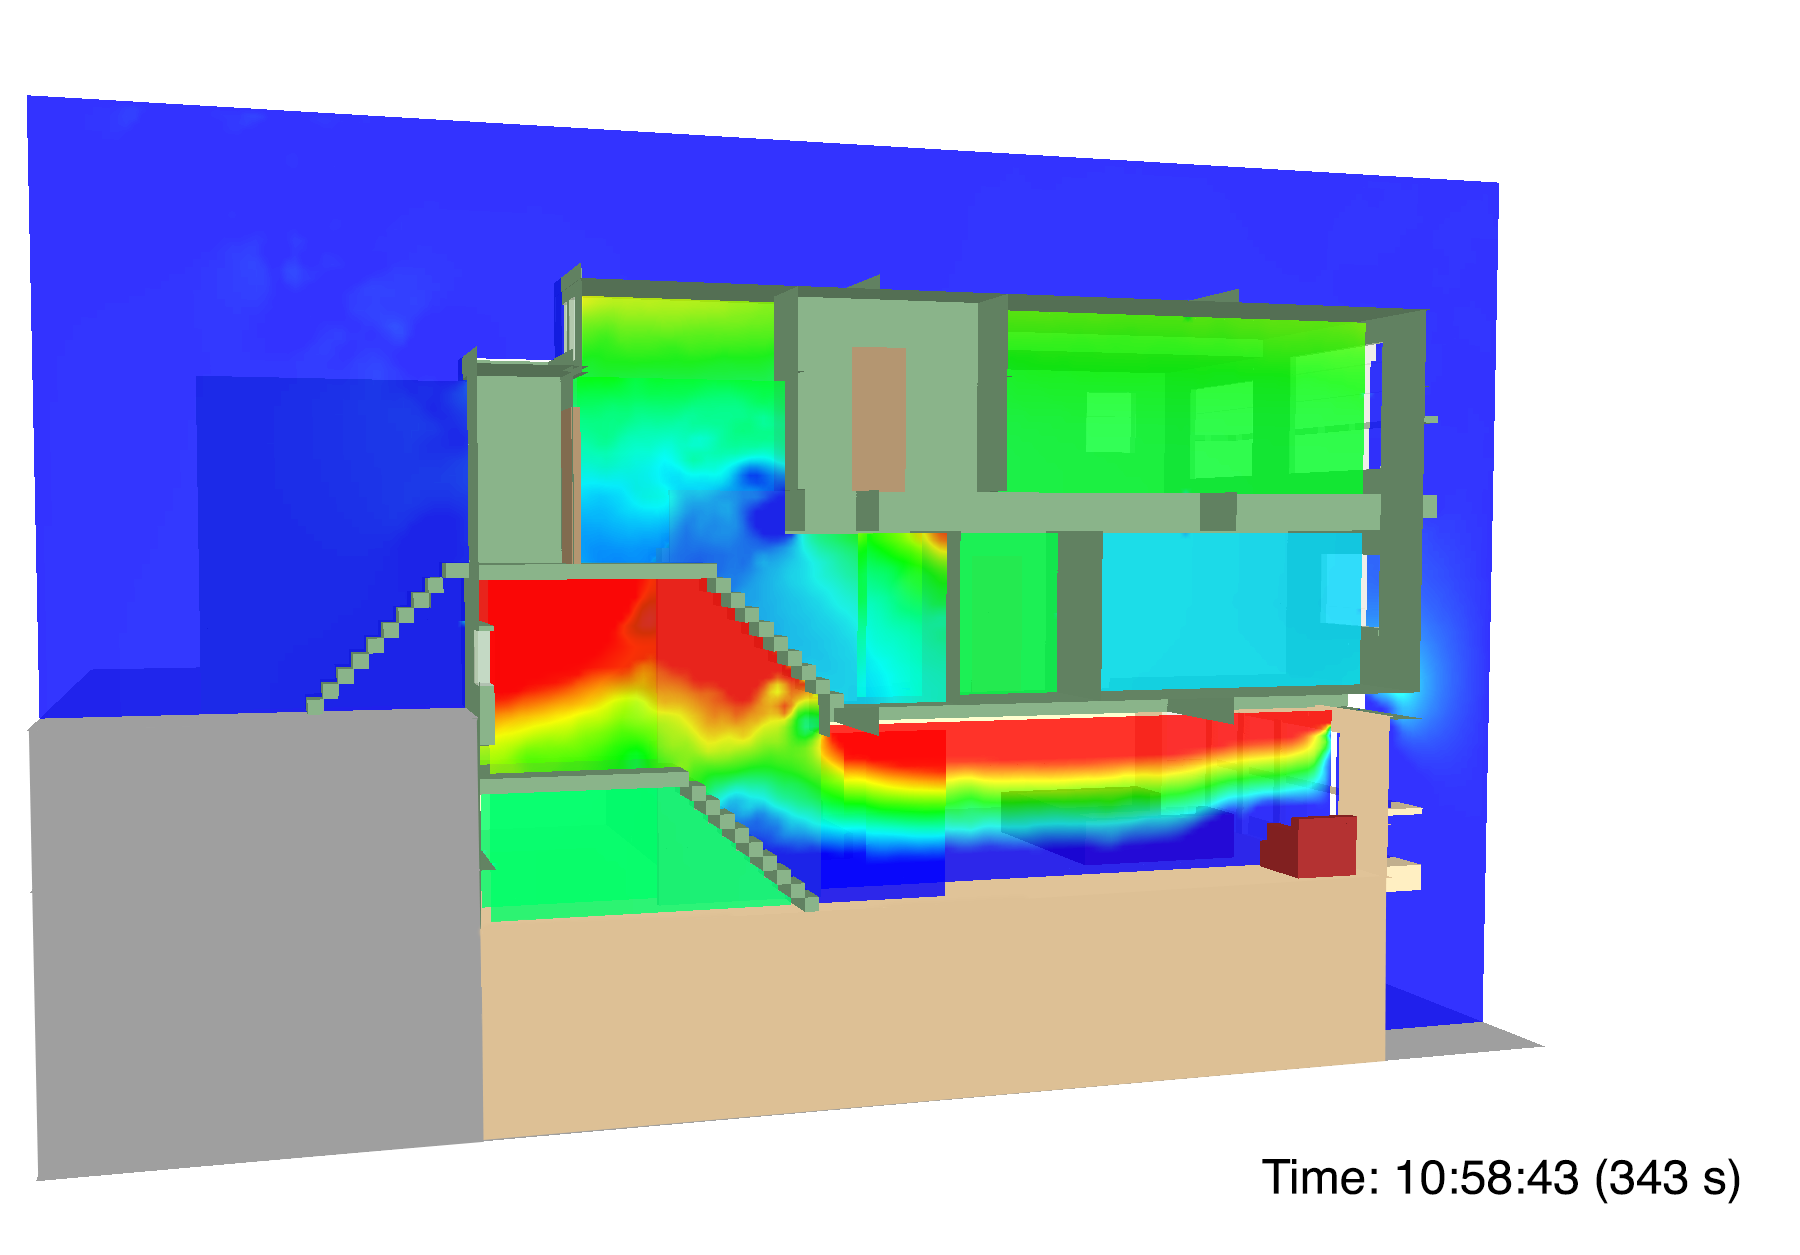
\includegraphics[width=5.5in]{../Figures/SMV_Pres_343_s}
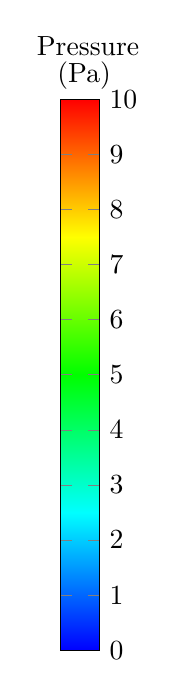
\begin{tikzpicture}
\pgfkeys{/pgf/number format/set thousands separator = {}}
\node at (0.65,0.67) {Pressure};
\node at (0.6,0.3) {(Pa)};
\begin{axis}[
    hide axis,
    scale only axis,
    height=0pt,
    width=0pt,
    colorbar,
    point meta min=0,
    point meta max=10,
    colorbar style={
        height=7cm,
        ytick={0,1,2,...,10}}
    ]
    \addplot [draw=none] coordinates {(0,0)};
\end{axis}
\end{tikzpicture}

\caption{FDS simulated pressure contours, 2~s before (top) and 1~s after (bottom) first rear basement window failure (342~s). The fire originated in the living room in the basement.}
\label{fig:smv_pressure}
\end{figure}


\clearpage


\section{Velocity}
\label{sec:velocity}

Gases at an elevated pressure will flow towards a region of lower pressure. Once the rear basement windows failed, the gases in the basement at an elevated temperature and pressure flowed into the interior stairwell towards the low pressure regions in the house and exhausted via the garage door and front door. The velocity contours shown in Fig.~\ref{fig:smv_velocity} indicate the magnitude of flow velocities within the structure before and after the rear basement window failures.

In this figure, the velocity profile within the high hazard areas is shown via two snapshots in time to illustrate the change in the interior conditions. The first snapshot is shown at a time of 340~s into the simulation, which is 2~s before the first rear basement window failed, and the second snapshot is shown at a time of 402~s into the simulation, which is 60~s after the first rear basement window failed.

The velocity vectors shown in Fig.~\ref{fig:smv_velocity_vectors} indicate the direction and magnitude of flow velocities within the structure before and after the rear basement window failures. Based on Figs.~\ref{fig:smv_velocity} and \ref{fig:smv_velocity_vectors}, the maximum velocity in the interior stairwell was approximately 9~m/s (20 mph).

\begin{figure}[!ht]
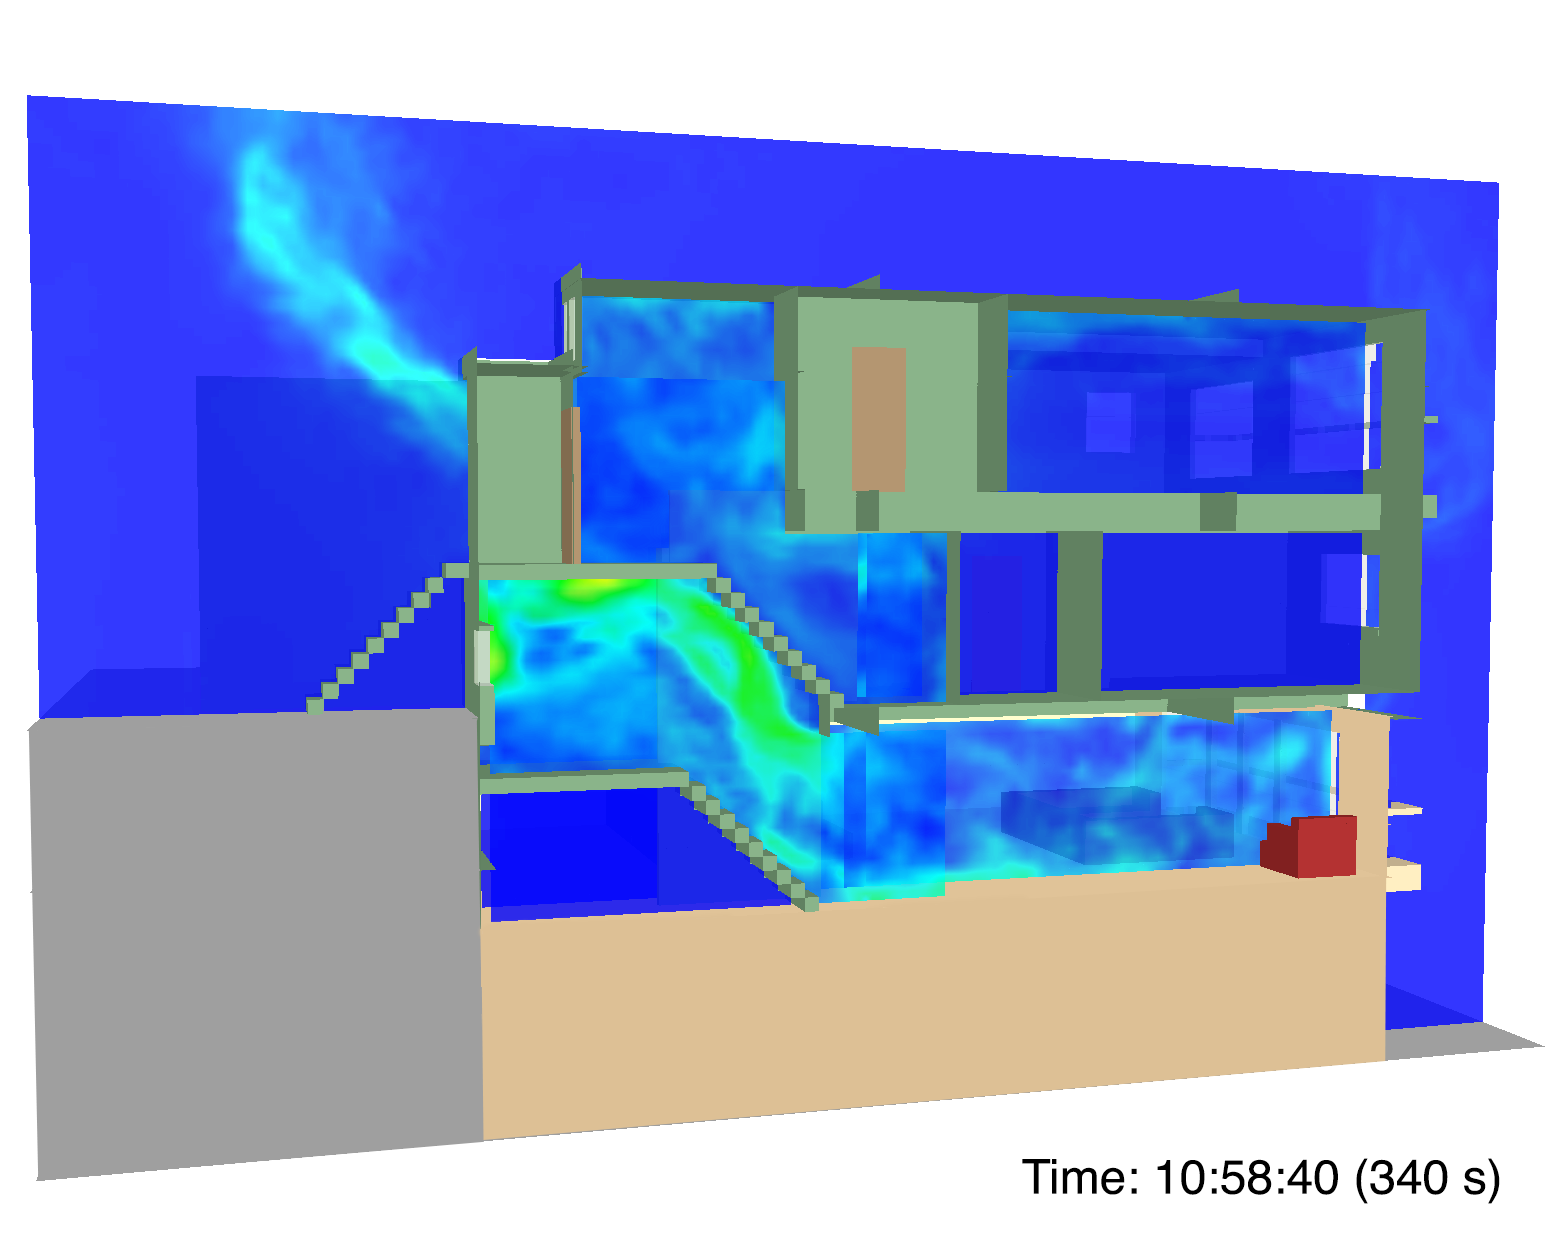
\includegraphics[width=4.5in]{../Figures/SMV_Vel_340_s}
%\documentclass{standalone}
%\usepackage{pgfplots}
%\begin{document}
%\pgfplotsset{
%	colormap={blackwhite}{[5pt]
%		rgb255(0pt)=(0,0,255); 
%		rgb255(100pt)=(0,255,255); 
%		rgb255(200pt)=(0,255,0); 
%		rgb255(300pt)=(255,255,0); 
%		rgb255(400pt)=(255,0,0)
%	},
%}
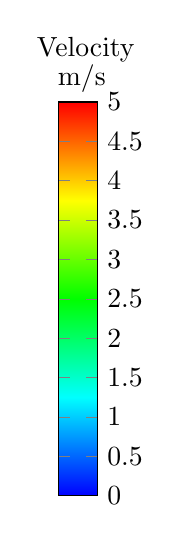
\begin{tikzpicture}
\node at (0.65,0.67) {Velocity};
\node at (0.6,0.3) {m/s};
\begin{axis}[
    hide axis,
    scale only axis,
    height=0pt,
    width=0pt,
    colorbar,
    point meta min=0,
    point meta max=5,
    colorbar style={
        height=5cm,
        ytick={0,0.5,1,...,5}
    }]
    \addplot [draw=none] coordinates {(0,0)};
\end{axis}
\end{tikzpicture}
%\end{document}

%\documentclass{standalone}
%\usepackage{pgfplots}
%\begin{document}
%\pgfplotsset{
%	colormap={blackwhite}{[5pt]
%		rgb255(0pt)=(0,0,255); 
%		rgb255(100pt)=(0,255,255); 
%		rgb255(200pt)=(0,255,0); 
%		rgb255(300pt)=(255,255,0); 
%		rgb255(400pt)=(255,0,0)
%	},
%}
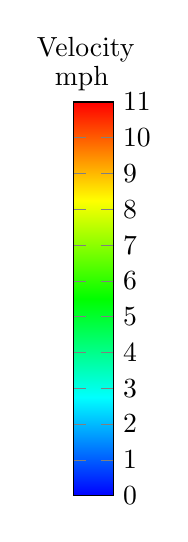
\begin{tikzpicture}
\node at (0.45,0.67) {Velocity};
\node at (0.4,0.3) {mph};
\begin{axis}[
    hide axis,
    scale only axis,
    height=0pt,
    width=0pt,
    colorbar,
    point meta min=0,
    point meta max=11,
    colorbar style={
        height=5cm,
        ytick={0,1,2,...,11}
    }]
    \addplot [draw=none] coordinates {(0,0)};
\end{axis}
\end{tikzpicture}
%\end{document}
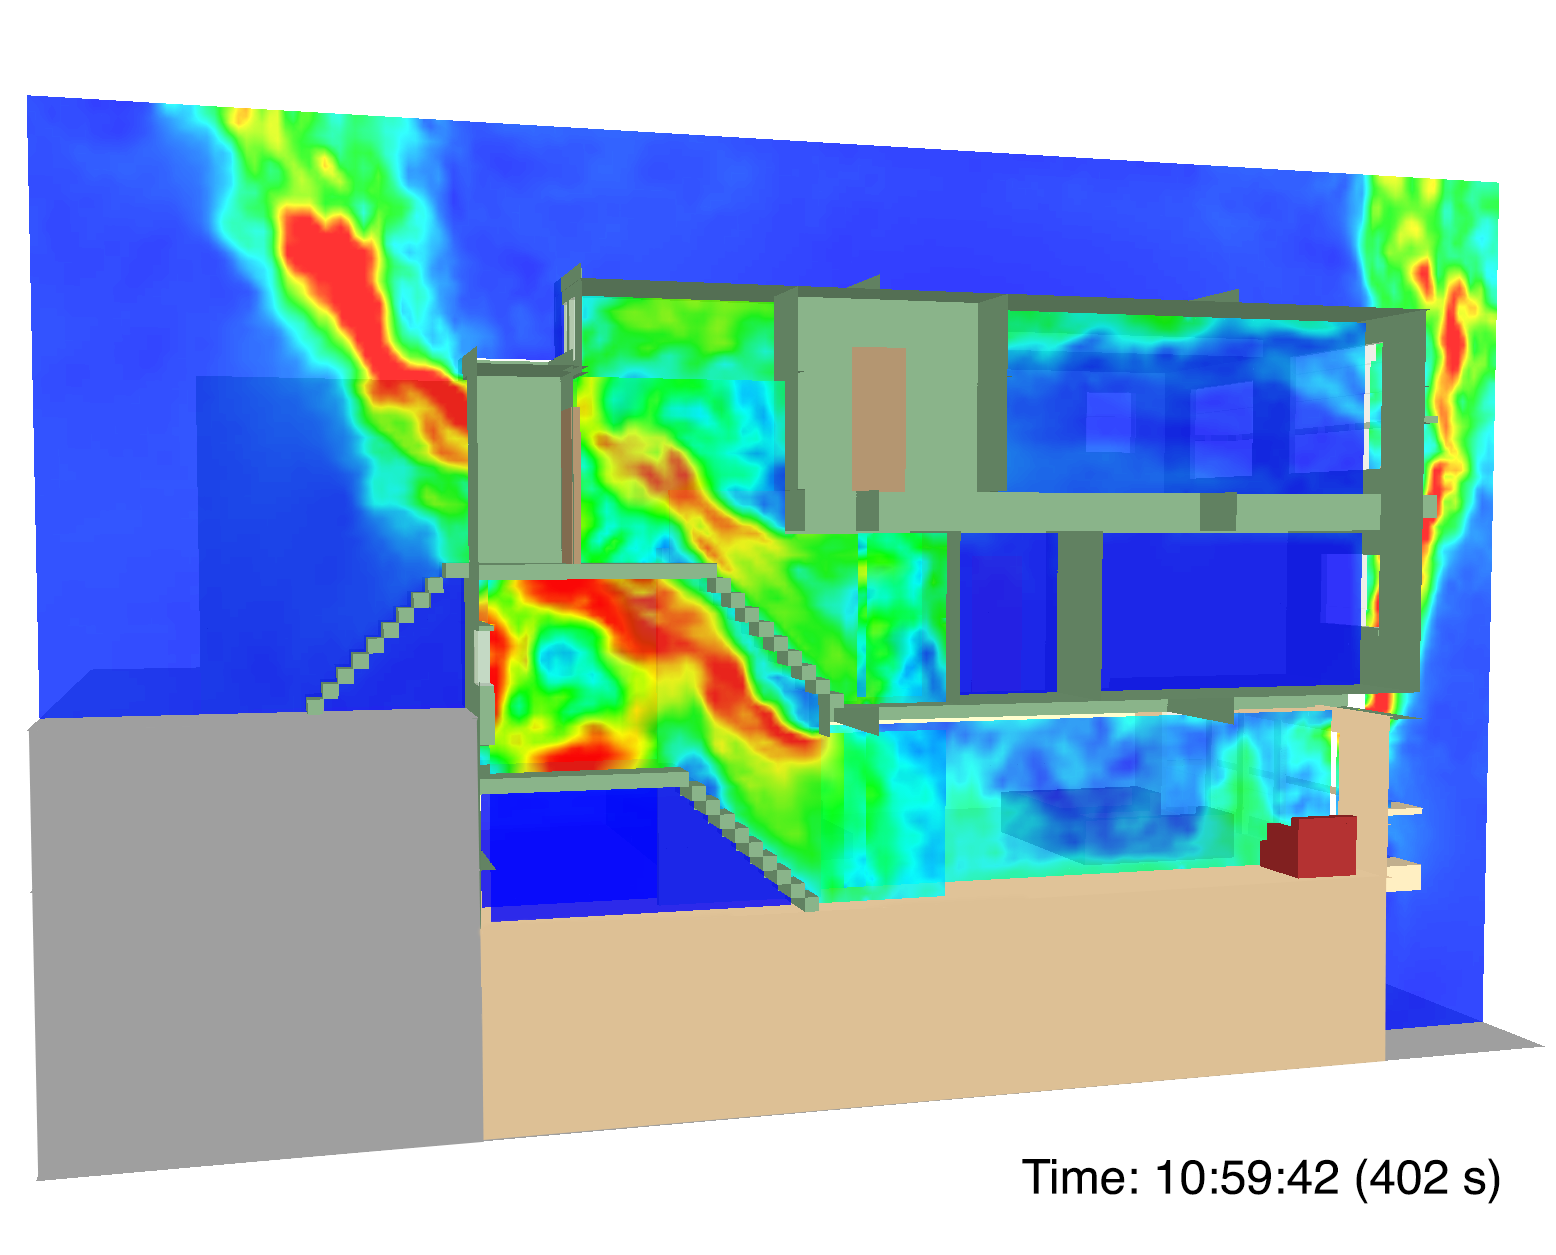
\includegraphics[width=4.5in]{../Figures/SMV_Vel_402_s}
%\documentclass{standalone}
%\usepackage{pgfplots}
%\begin{document}
%\pgfplotsset{
%	colormap={blackwhite}{[5pt]
%		rgb255(0pt)=(0,0,255); 
%		rgb255(100pt)=(0,255,255); 
%		rgb255(200pt)=(0,255,0); 
%		rgb255(300pt)=(255,255,0); 
%		rgb255(400pt)=(255,0,0)
%	},
%}
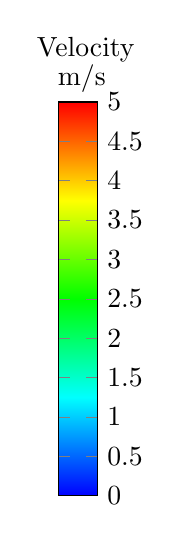
\begin{tikzpicture}
\node at (0.65,0.67) {Velocity};
\node at (0.6,0.3) {m/s};
\begin{axis}[
    hide axis,
    scale only axis,
    height=0pt,
    width=0pt,
    colorbar,
    point meta min=0,
    point meta max=5,
    colorbar style={
        height=5cm,
        ytick={0,0.5,1,...,5}
    }]
    \addplot [draw=none] coordinates {(0,0)};
\end{axis}
\end{tikzpicture}
%\end{document}

%\documentclass{standalone}
%\usepackage{pgfplots}
%\begin{document}
%\pgfplotsset{
%	colormap={blackwhite}{[5pt]
%		rgb255(0pt)=(0,0,255); 
%		rgb255(100pt)=(0,255,255); 
%		rgb255(200pt)=(0,255,0); 
%		rgb255(300pt)=(255,255,0); 
%		rgb255(400pt)=(255,0,0)
%	},
%}
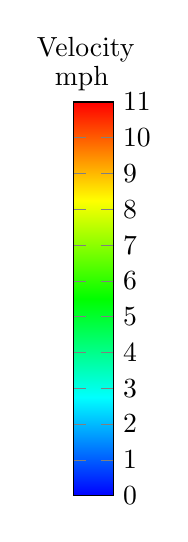
\begin{tikzpicture}
\node at (0.45,0.67) {Velocity};
\node at (0.4,0.3) {mph};
\begin{axis}[
    hide axis,
    scale only axis,
    height=0pt,
    width=0pt,
    colorbar,
    point meta min=0,
    point meta max=11,
    colorbar style={
        height=5cm,
        ytick={0,1,2,...,11}
    }]
    \addplot [draw=none] coordinates {(0,0)};
\end{axis}
\end{tikzpicture}
%\end{document}
\caption{FDS simulated velocity contours, 2~s before (top) and 60~s after (bottom) first rear basement window failure (342~s).}
\label{fig:smv_velocity}
\end{figure}


\clearpage


\begin{figure}[!ht]
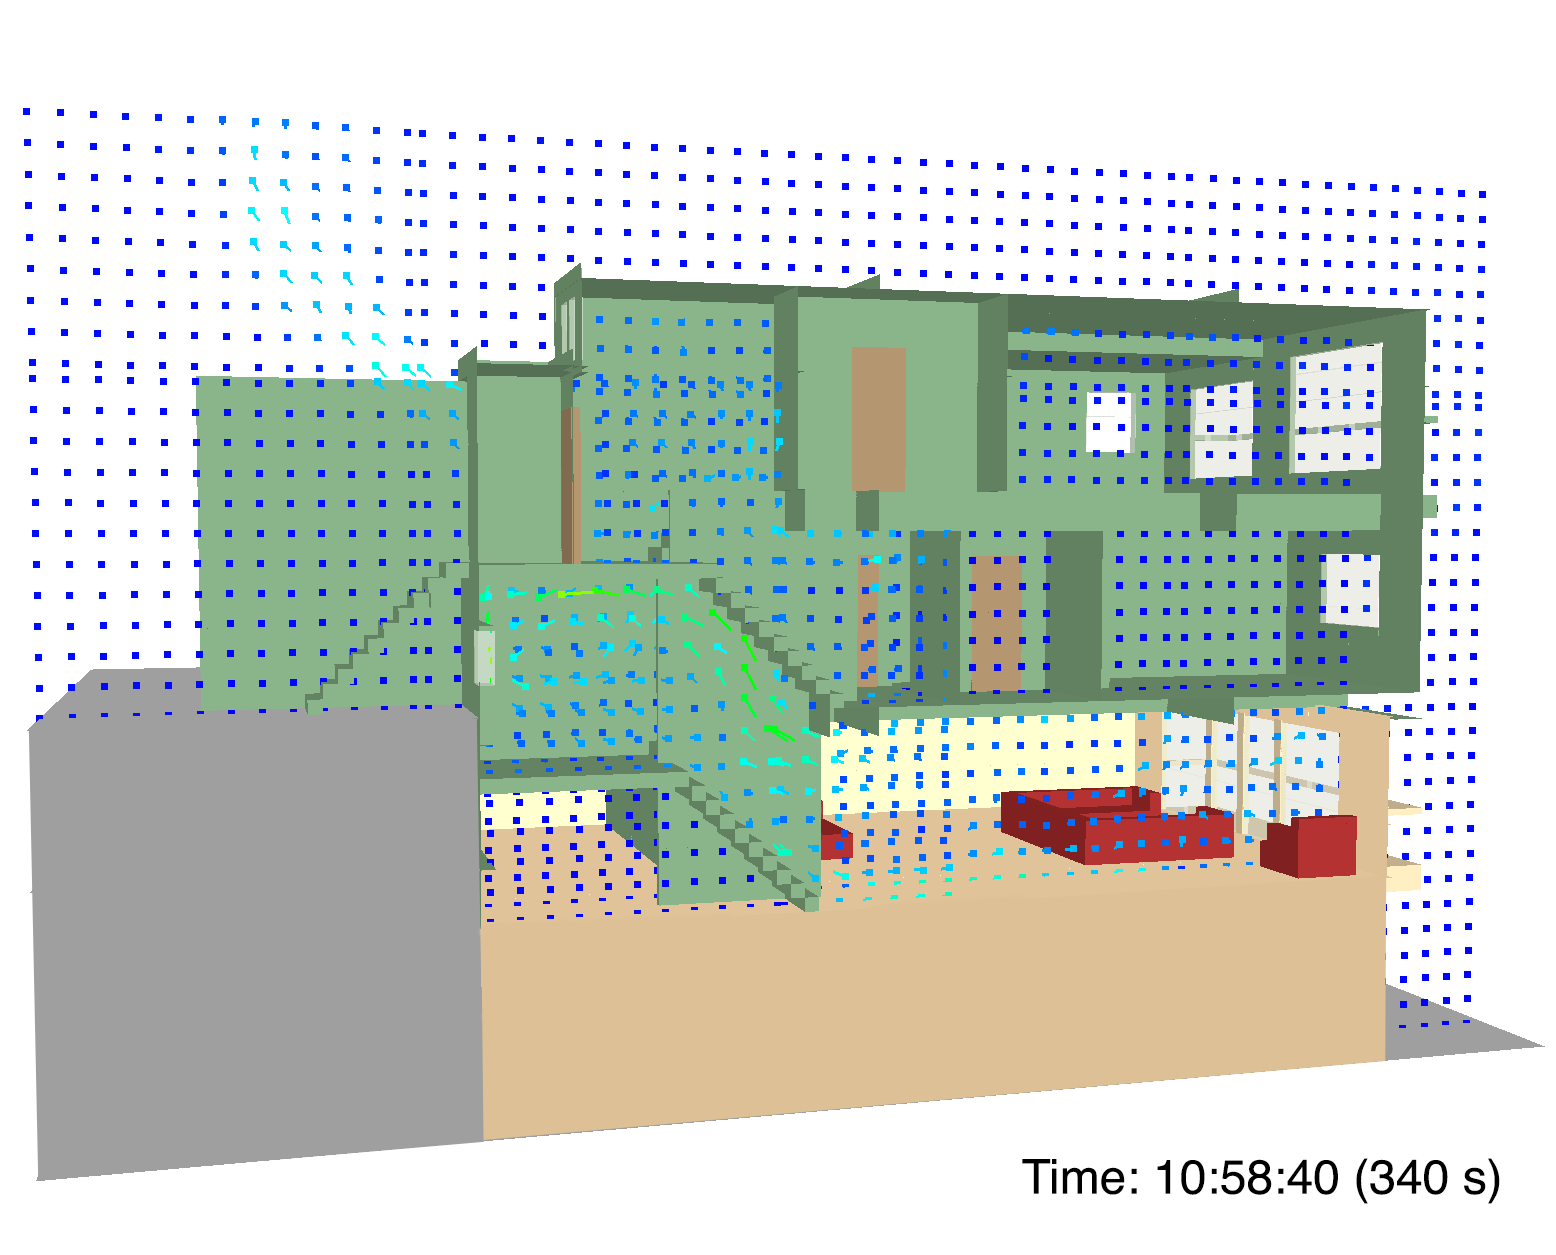
\includegraphics[width=4.5in]{../Figures/SMV_Vel_Vec_340_s}
%\documentclass{standalone}
%\usepackage{pgfplots}
%\begin{document}
%\pgfplotsset{
%	colormap={blackwhite}{[5pt]
%		rgb255(0pt)=(0,0,255); 
%		rgb255(100pt)=(0,255,255); 
%		rgb255(200pt)=(0,255,0); 
%		rgb255(300pt)=(255,255,0); 
%		rgb255(400pt)=(255,0,0)
%	},
%}
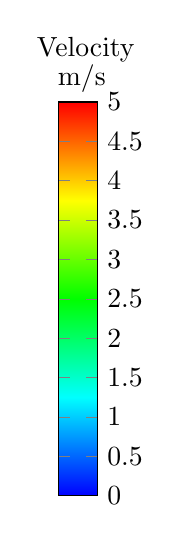
\begin{tikzpicture}
\node at (0.65,0.67) {Velocity};
\node at (0.6,0.3) {m/s};
\begin{axis}[
    hide axis,
    scale only axis,
    height=0pt,
    width=0pt,
    colorbar,
    point meta min=0,
    point meta max=5,
    colorbar style={
        height=5cm,
        ytick={0,0.5,1,...,5}
    }]
    \addplot [draw=none] coordinates {(0,0)};
\end{axis}
\end{tikzpicture}
%\end{document}

%\documentclass{standalone}
%\usepackage{pgfplots}
%\begin{document}
%\pgfplotsset{
%	colormap={blackwhite}{[5pt]
%		rgb255(0pt)=(0,0,255); 
%		rgb255(100pt)=(0,255,255); 
%		rgb255(200pt)=(0,255,0); 
%		rgb255(300pt)=(255,255,0); 
%		rgb255(400pt)=(255,0,0)
%	},
%}
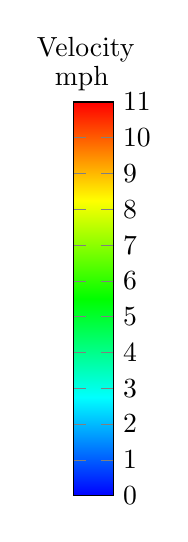
\begin{tikzpicture}
\node at (0.45,0.67) {Velocity};
\node at (0.4,0.3) {mph};
\begin{axis}[
    hide axis,
    scale only axis,
    height=0pt,
    width=0pt,
    colorbar,
    point meta min=0,
    point meta max=11,
    colorbar style={
        height=5cm,
        ytick={0,1,2,...,11}
    }]
    \addplot [draw=none] coordinates {(0,0)};
\end{axis}
\end{tikzpicture}
%\end{document}
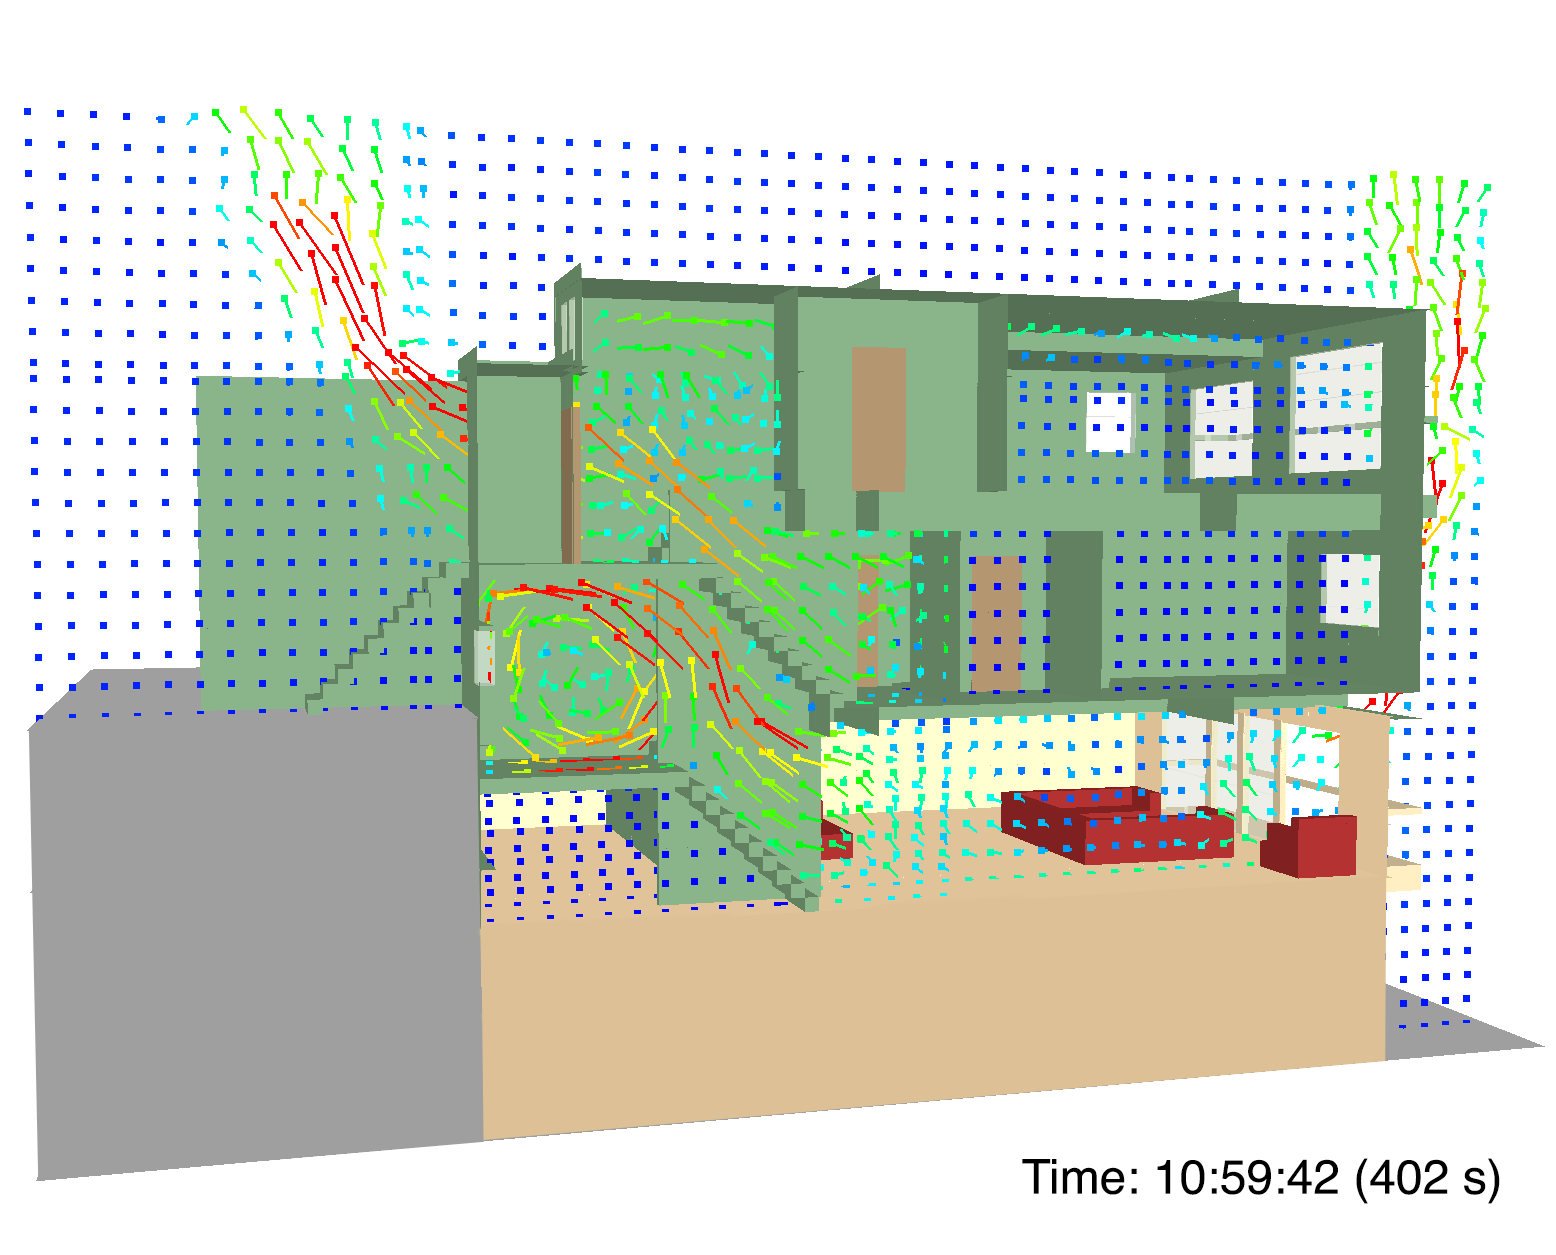
\includegraphics[width=4.5in]{../Figures/SMV_Vel_Vec_402_s}
%\documentclass{standalone}
%\usepackage{pgfplots}
%\begin{document}
%\pgfplotsset{
%	colormap={blackwhite}{[5pt]
%		rgb255(0pt)=(0,0,255); 
%		rgb255(100pt)=(0,255,255); 
%		rgb255(200pt)=(0,255,0); 
%		rgb255(300pt)=(255,255,0); 
%		rgb255(400pt)=(255,0,0)
%	},
%}
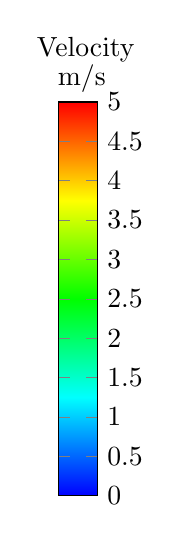
\begin{tikzpicture}
\node at (0.65,0.67) {Velocity};
\node at (0.6,0.3) {m/s};
\begin{axis}[
    hide axis,
    scale only axis,
    height=0pt,
    width=0pt,
    colorbar,
    point meta min=0,
    point meta max=5,
    colorbar style={
        height=5cm,
        ytick={0,0.5,1,...,5}
    }]
    \addplot [draw=none] coordinates {(0,0)};
\end{axis}
\end{tikzpicture}
%\end{document}

%\documentclass{standalone}
%\usepackage{pgfplots}
%\begin{document}
%\pgfplotsset{
%	colormap={blackwhite}{[5pt]
%		rgb255(0pt)=(0,0,255); 
%		rgb255(100pt)=(0,255,255); 
%		rgb255(200pt)=(0,255,0); 
%		rgb255(300pt)=(255,255,0); 
%		rgb255(400pt)=(255,0,0)
%	},
%}
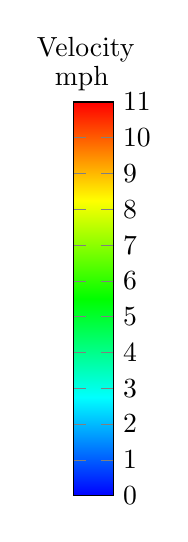
\begin{tikzpicture}
\node at (0.45,0.67) {Velocity};
\node at (0.4,0.3) {mph};
\begin{axis}[
    hide axis,
    scale only axis,
    height=0pt,
    width=0pt,
    colorbar,
    point meta min=0,
    point meta max=11,
    colorbar style={
        height=5cm,
        ytick={0,1,2,...,11}
    }]
    \addplot [draw=none] coordinates {(0,0)};
\end{axis}
\end{tikzpicture}
%\end{document}
\caption{FDS simulated velocity vectors, 2~s before (top) and 60~s after (bottom) first rear basement window failure (342~s).}
\label{fig:smv_velocity_vectors}
\end{figure}


\clearpage


\section{Temperature}
\label{sec:temperature}

Analysis of the temperatures from the simulation focuses on the high hazard areas of the structure: the basement and the interior stairwell which connects the basement to the exhaust vents/doors on the front side of the structure (the front door and the garage door). The temperature contours shown in Fig.~\ref{fig:smv_temperature} indicate the gas temperatures within the structure before and after the rear basement window failures.

In this figure, The temperature profile at these high hazard areas is shown via two snapshots in time to illustrate the change in the interior conditions. The first snapshot is shown at a time of 340~s into the simulation, which is 2~s before the first rear basement window failed, and the second snapshot is shown at a time of 402~s into the simulation, which is 60~s after the first rear basement window failed.

The temperature vectors shown in Fig.~\ref{fig:smv_temperature_vectors} indicate the gas temperatures and direction of flow within the structure before and after the rear basement window failures. Based on the results shown in Figs.~\ref{fig:smv_temperature} and \ref{fig:smv_temperature_vectors} after the rear basement windows began to fail, the maximum temperature in the basement was in excess of 800~$^{\circ}$C (1500~$^{\circ}$F), and the maximum temperature in the interior stairwell was in excess of 600~$^{\circ}$C (1100~$^{\circ}$F).

\begin{figure}[!ht]
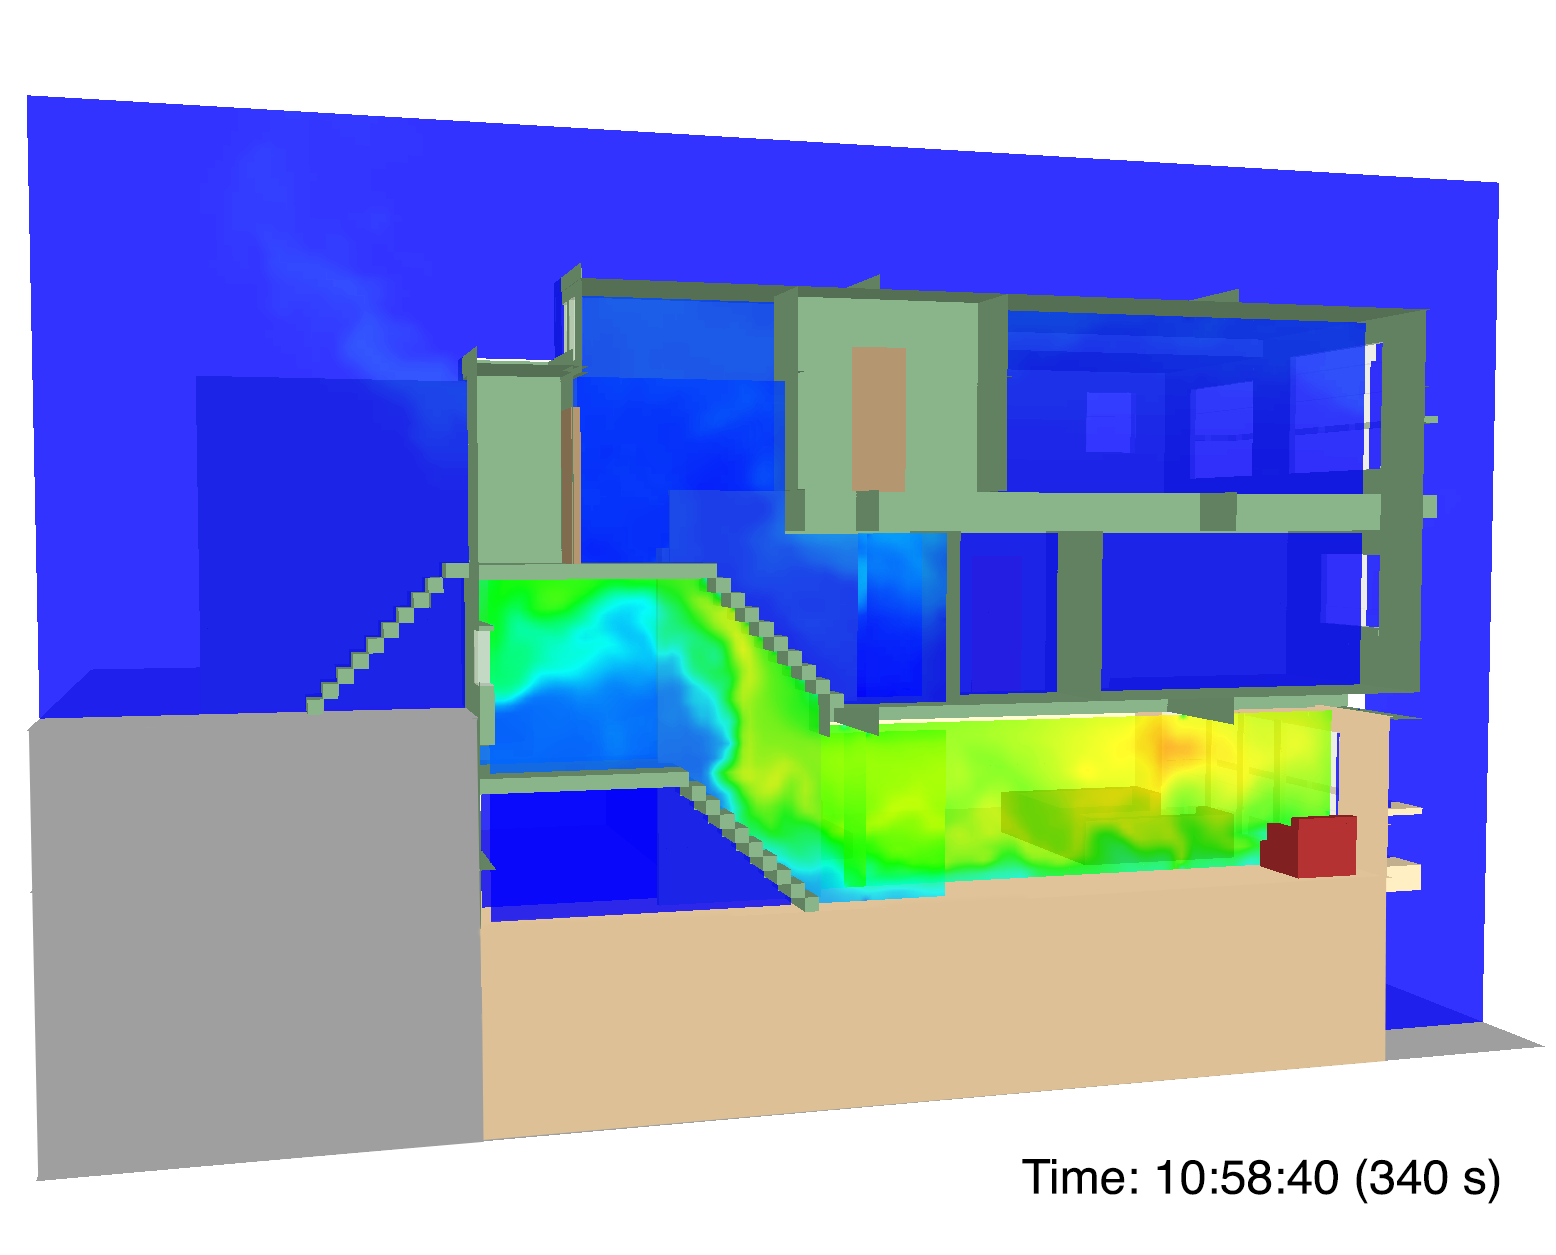
\includegraphics[width=4.3in]{../Figures/SMV_Temp_340_s}
%\documentclass{standalone}
%\usepackage{pgfplots}
%\begin{document}
%\pgfplotsset{
%	colormap={blackwhite}{[5pt]
%		rgb255(0pt)=(0,0,255); 
%		rgb255(100pt)=(0,255,255); 
%		rgb255(200pt)=(0,255,0); 
%		rgb255(300pt)=(255,255,0); 
%		rgb255(400pt)=(255,0,0)
%	},
%}
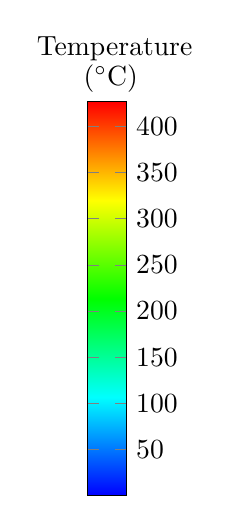
\begin{tikzpicture}
\node at (0.65,0.67) {Temperature};
\node at (0.6,0.3) {($^\circ$C)};
\begin{axis}[
    hide axis,
    scale only axis,
    height=0pt,
    width=0pt,
    colorbar,
    point meta min=0,
    point meta max=426.667,
    colorbar style={
        height=5cm,
        ytick={50,100,...,450}
    }]
    \addplot [draw=none] coordinates {(0,0)};
\end{axis}
\end{tikzpicture}
%\end{document}

%\documentclass{standalone}
%\usepackage{pgfplots}
%\begin{document}
%\pgfplotsset{
%	colormap={blackwhite}{[5pt]
%		rgb255(0pt)=(0,0,255); 
%		rgb255(100pt)=(0,255,255); 
%		rgb255(200pt)=(0,255,0); 
%		rgb255(300pt)=(255,255,0); 
%		rgb255(400pt)=(255,0,0)
%	},
%}
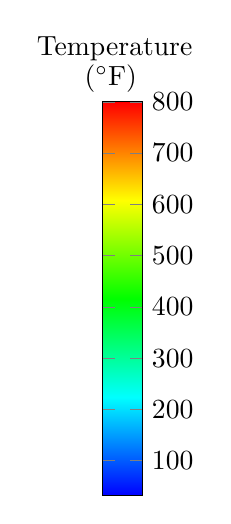
\begin{tikzpicture}
\node at (0.45,0.67) {Temperature};
\node at (0.4,0.3) {($^\circ$F)};
\begin{axis}[
    hide axis,
    scale only axis,
    height=0pt,
    width=0pt,
    colorbar,
    point meta min=32,
    point meta max=800,
    colorbar style={
        height=5cm,
        ytick={100,200,...,800}
    }]
    \addplot [draw=none] coordinates {(0,0)};
\end{axis}
\end{tikzpicture}
%\end{document}
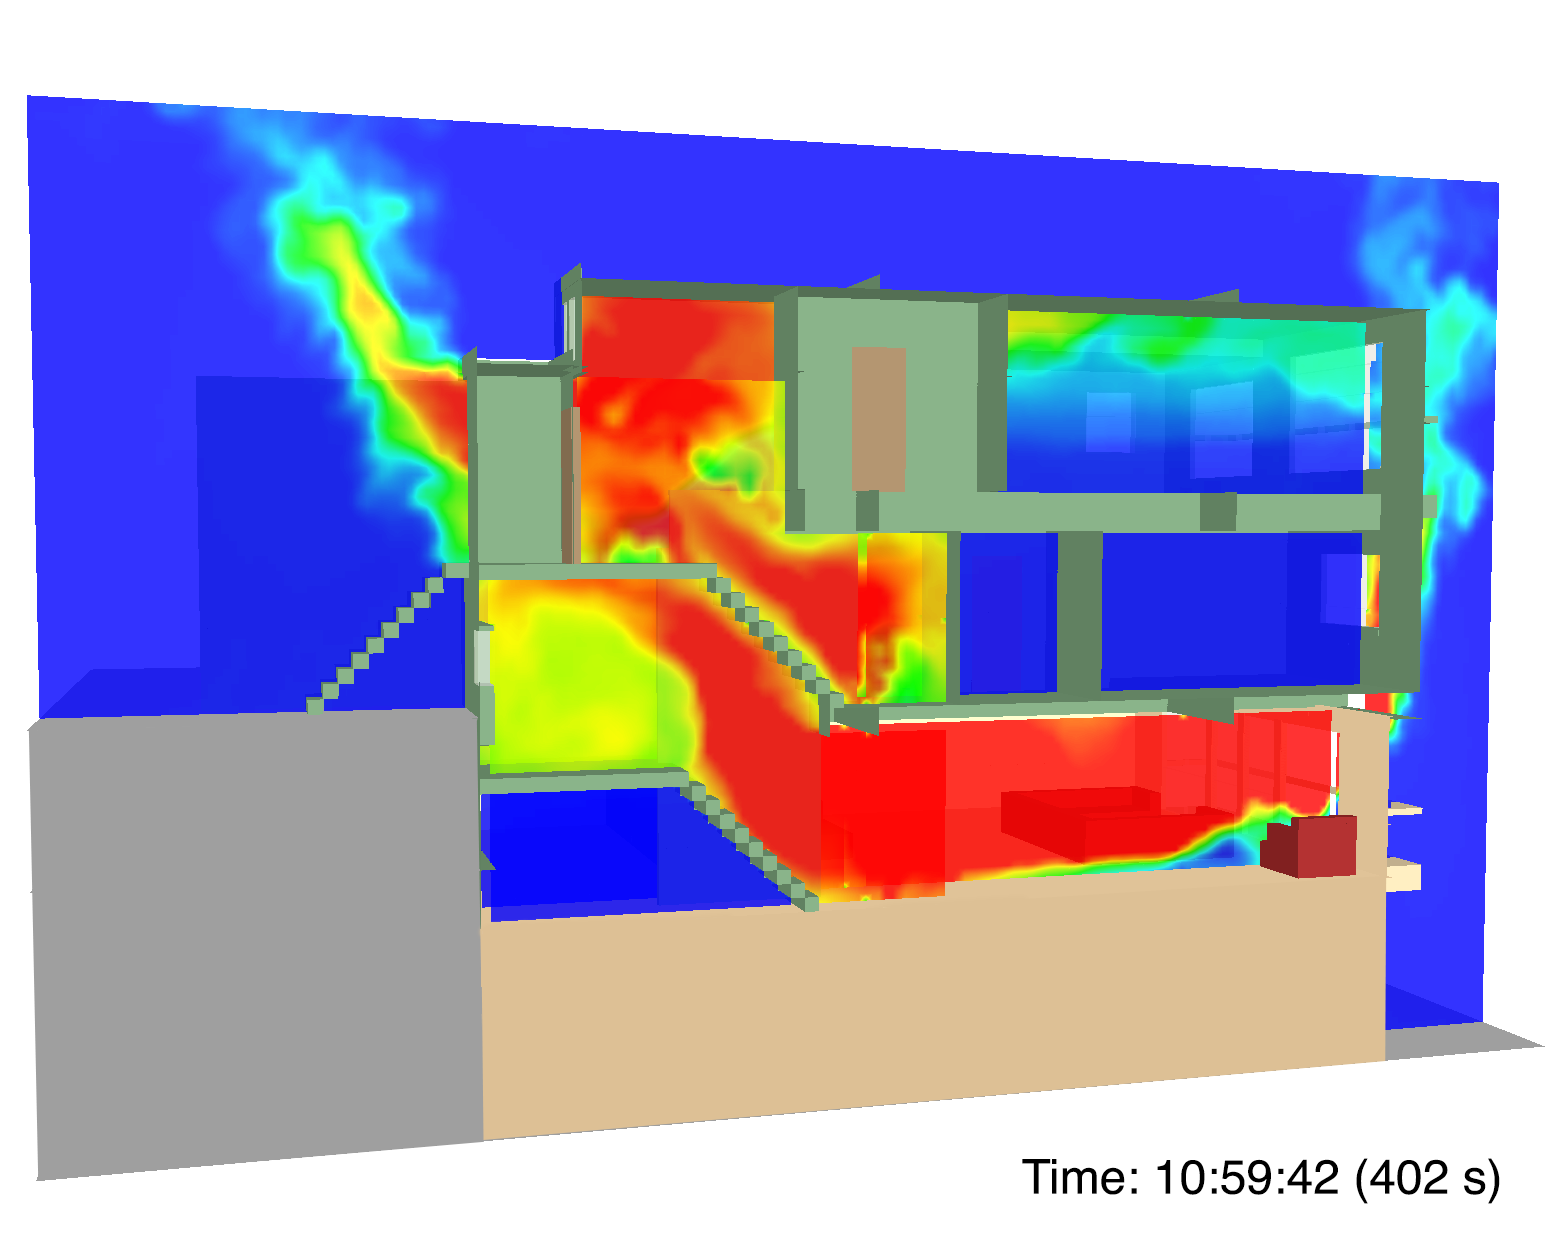
\includegraphics[width=4.3in]{../Figures/SMV_Temp_402_s}
%\documentclass{standalone}
%\usepackage{pgfplots}
%\begin{document}
%\pgfplotsset{
%	colormap={blackwhite}{[5pt]
%		rgb255(0pt)=(0,0,255); 
%		rgb255(100pt)=(0,255,255); 
%		rgb255(200pt)=(0,255,0); 
%		rgb255(300pt)=(255,255,0); 
%		rgb255(400pt)=(255,0,0)
%	},
%}
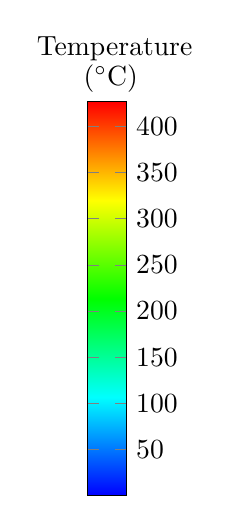
\begin{tikzpicture}
\node at (0.65,0.67) {Temperature};
\node at (0.6,0.3) {($^\circ$C)};
\begin{axis}[
    hide axis,
    scale only axis,
    height=0pt,
    width=0pt,
    colorbar,
    point meta min=0,
    point meta max=426.667,
    colorbar style={
        height=5cm,
        ytick={50,100,...,450}
    }]
    \addplot [draw=none] coordinates {(0,0)};
\end{axis}
\end{tikzpicture}
%\end{document}

%\documentclass{standalone}
%\usepackage{pgfplots}
%\begin{document}
%\pgfplotsset{
%	colormap={blackwhite}{[5pt]
%		rgb255(0pt)=(0,0,255); 
%		rgb255(100pt)=(0,255,255); 
%		rgb255(200pt)=(0,255,0); 
%		rgb255(300pt)=(255,255,0); 
%		rgb255(400pt)=(255,0,0)
%	},
%}
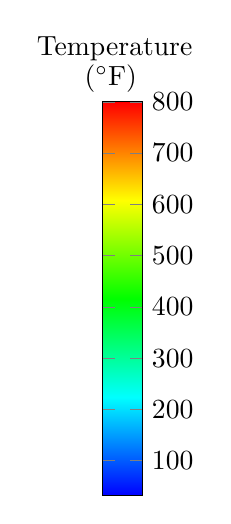
\begin{tikzpicture}
\node at (0.45,0.67) {Temperature};
\node at (0.4,0.3) {($^\circ$F)};
\begin{axis}[
    hide axis,
    scale only axis,
    height=0pt,
    width=0pt,
    colorbar,
    point meta min=32,
    point meta max=800,
    colorbar style={
        height=5cm,
        ytick={100,200,...,800}
    }]
    \addplot [draw=none] coordinates {(0,0)};
\end{axis}
\end{tikzpicture}
%\end{document}
\caption{FDS simulated temperature contours, 2~s before (top) and 60~s after (bottom) first rear basement window failure (342~s).}
\label{fig:smv_temperature}
\end{figure}


\clearpage


\begin{figure}[!ht]
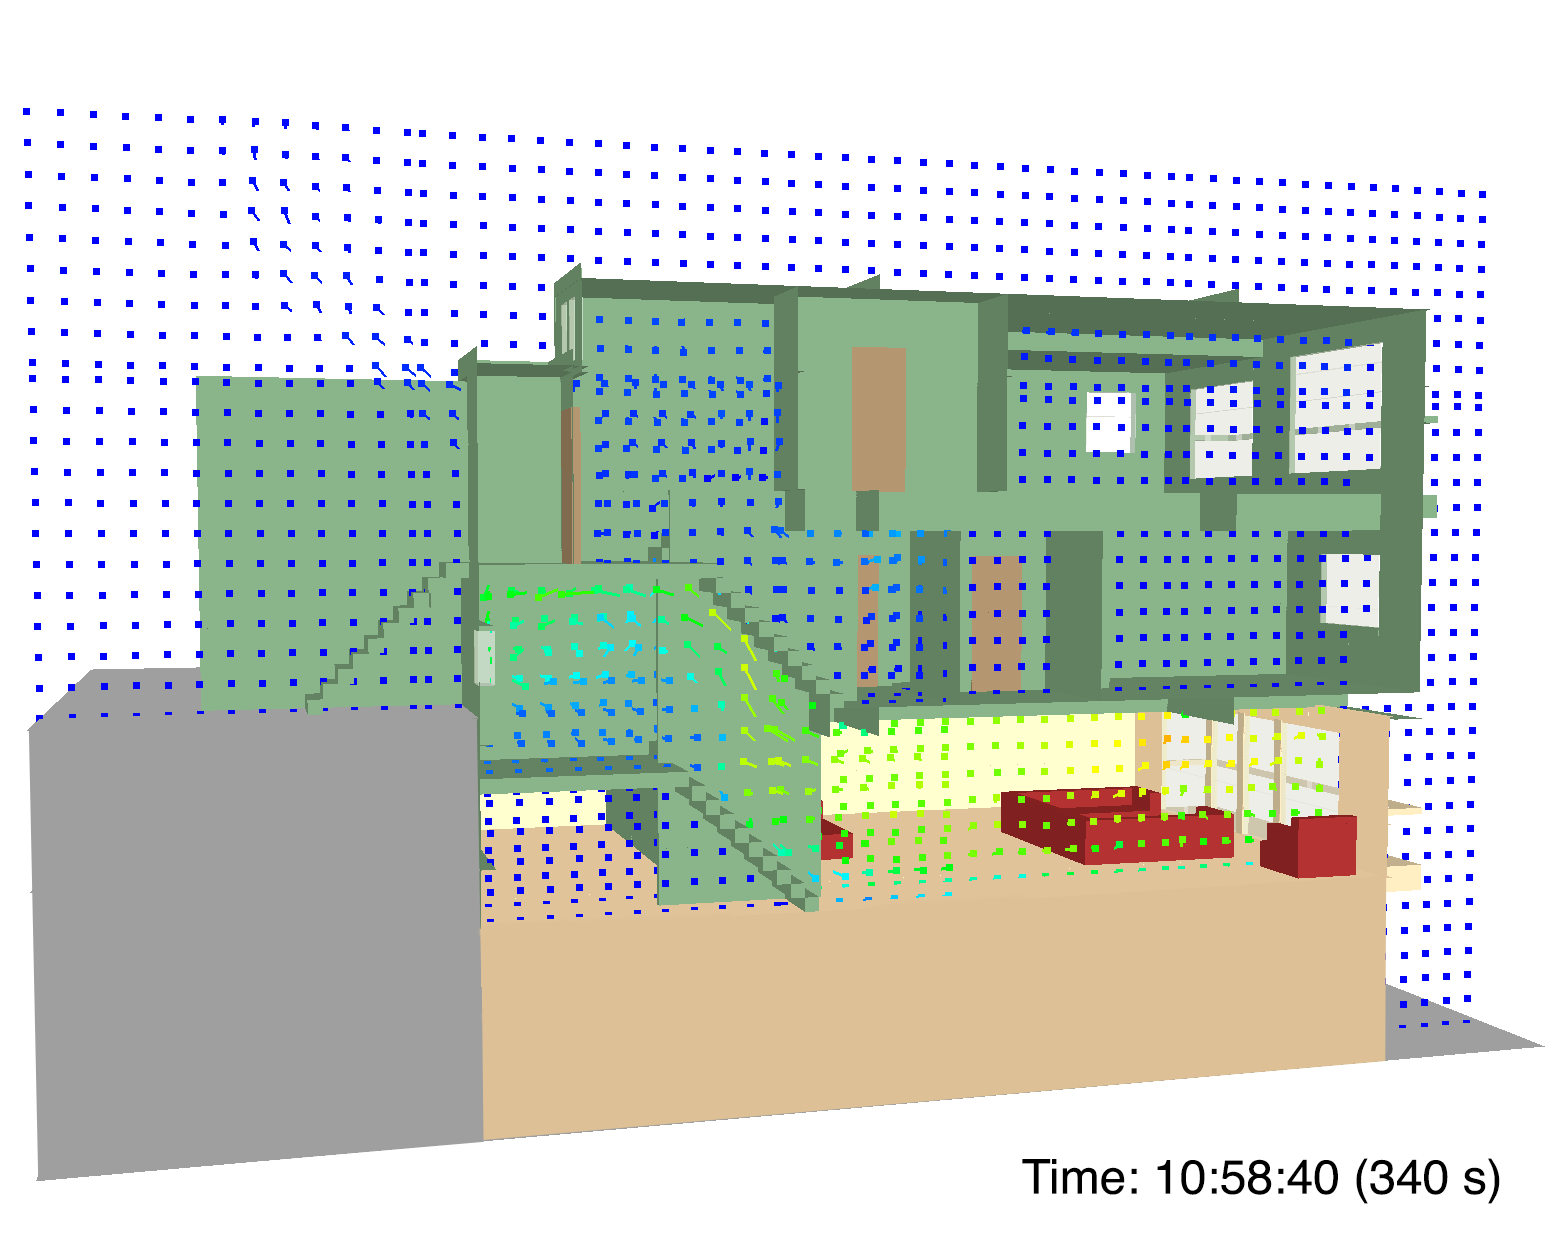
\includegraphics[width=4.3in]{../Figures/SMV_Temp_Vec_340_s}
%\documentclass{standalone}
%\usepackage{pgfplots}
%\begin{document}
%\pgfplotsset{
%	colormap={blackwhite}{[5pt]
%		rgb255(0pt)=(0,0,255); 
%		rgb255(100pt)=(0,255,255); 
%		rgb255(200pt)=(0,255,0); 
%		rgb255(300pt)=(255,255,0); 
%		rgb255(400pt)=(255,0,0)
%	},
%}
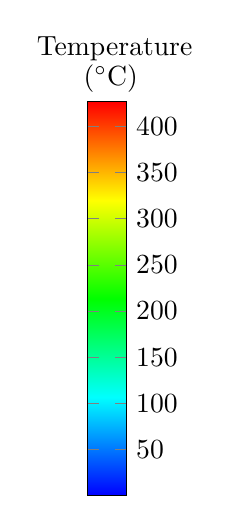
\begin{tikzpicture}
\node at (0.65,0.67) {Temperature};
\node at (0.6,0.3) {($^\circ$C)};
\begin{axis}[
    hide axis,
    scale only axis,
    height=0pt,
    width=0pt,
    colorbar,
    point meta min=0,
    point meta max=426.667,
    colorbar style={
        height=5cm,
        ytick={50,100,...,450}
    }]
    \addplot [draw=none] coordinates {(0,0)};
\end{axis}
\end{tikzpicture}
%\end{document}

%\documentclass{standalone}
%\usepackage{pgfplots}
%\begin{document}
%\pgfplotsset{
%	colormap={blackwhite}{[5pt]
%		rgb255(0pt)=(0,0,255); 
%		rgb255(100pt)=(0,255,255); 
%		rgb255(200pt)=(0,255,0); 
%		rgb255(300pt)=(255,255,0); 
%		rgb255(400pt)=(255,0,0)
%	},
%}
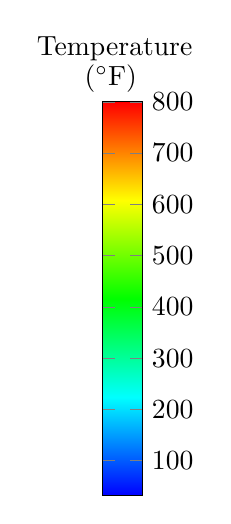
\begin{tikzpicture}
\node at (0.45,0.67) {Temperature};
\node at (0.4,0.3) {($^\circ$F)};
\begin{axis}[
    hide axis,
    scale only axis,
    height=0pt,
    width=0pt,
    colorbar,
    point meta min=32,
    point meta max=800,
    colorbar style={
        height=5cm,
        ytick={100,200,...,800}
    }]
    \addplot [draw=none] coordinates {(0,0)};
\end{axis}
\end{tikzpicture}
%\end{document}
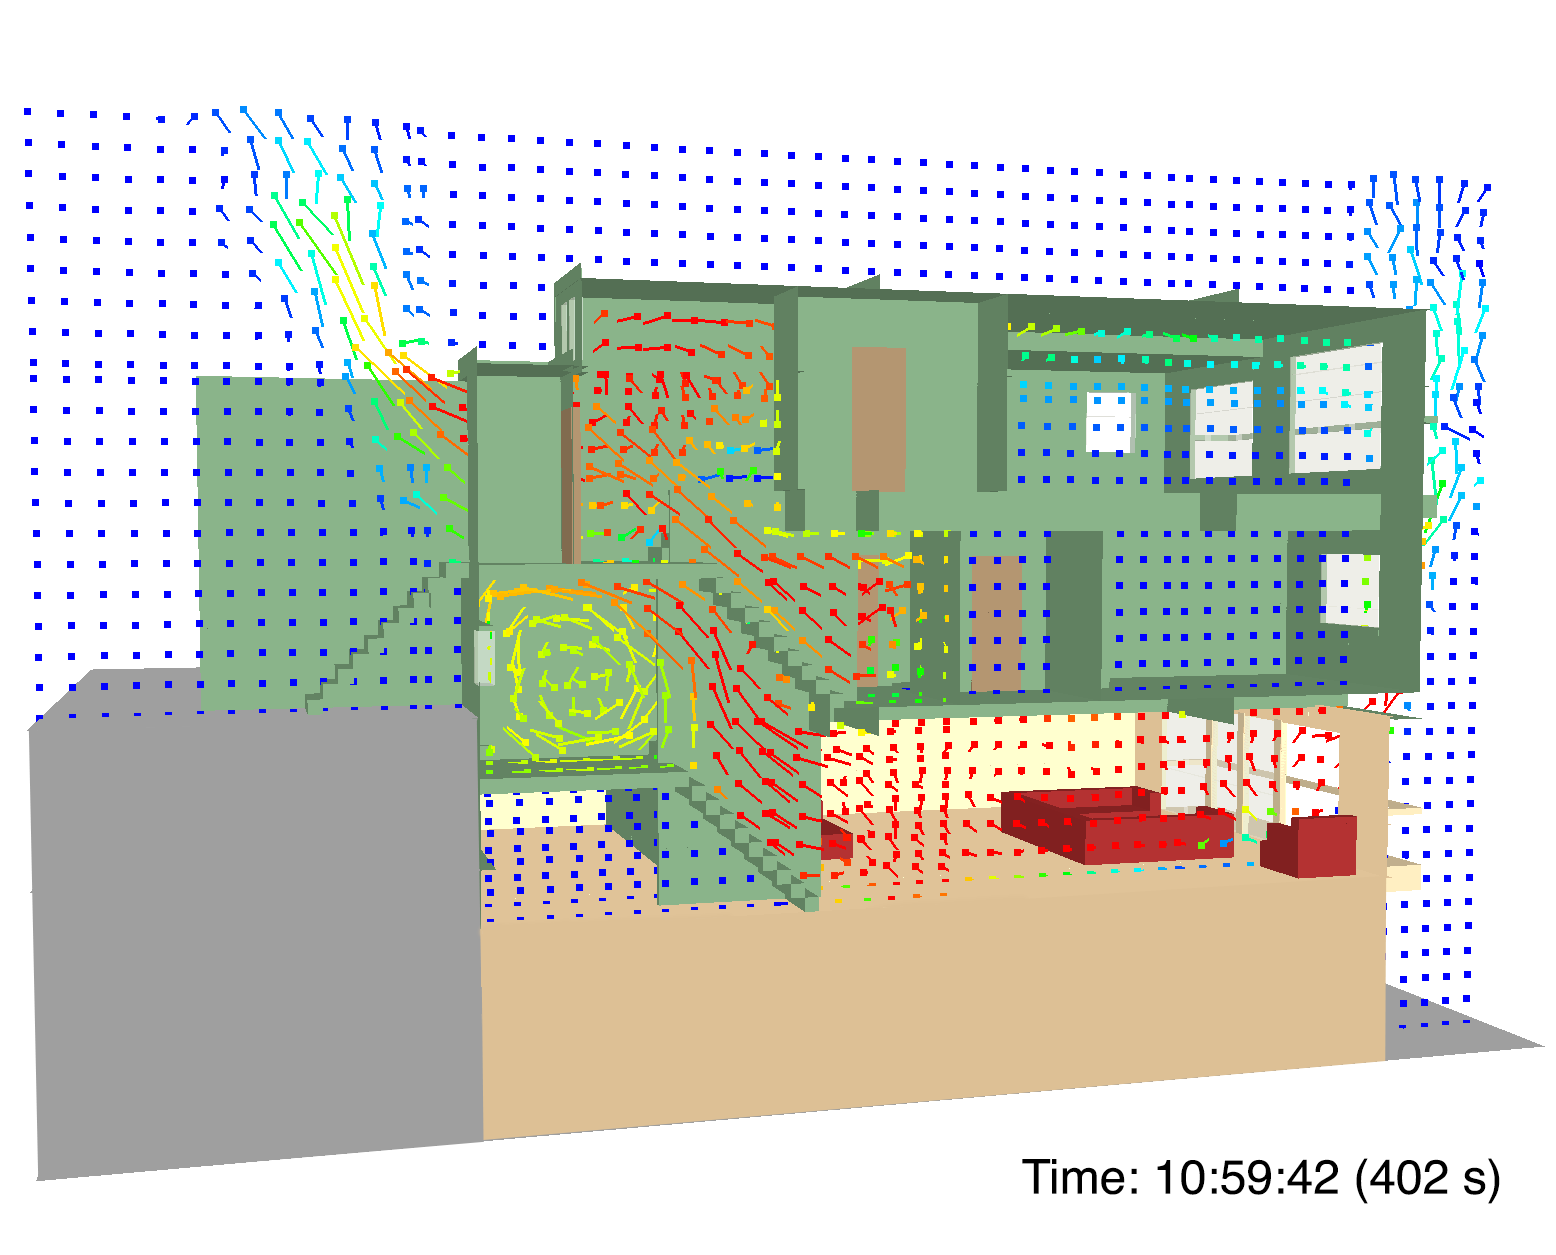
\includegraphics[width=4.3in]{../Figures/SMV_Temp_Vec_402_s}
%\documentclass{standalone}
%\usepackage{pgfplots}
%\begin{document}
%\pgfplotsset{
%	colormap={blackwhite}{[5pt]
%		rgb255(0pt)=(0,0,255); 
%		rgb255(100pt)=(0,255,255); 
%		rgb255(200pt)=(0,255,0); 
%		rgb255(300pt)=(255,255,0); 
%		rgb255(400pt)=(255,0,0)
%	},
%}
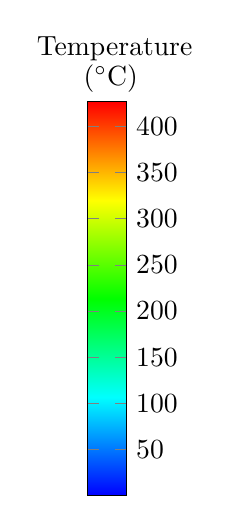
\begin{tikzpicture}
\node at (0.65,0.67) {Temperature};
\node at (0.6,0.3) {($^\circ$C)};
\begin{axis}[
    hide axis,
    scale only axis,
    height=0pt,
    width=0pt,
    colorbar,
    point meta min=0,
    point meta max=426.667,
    colorbar style={
        height=5cm,
        ytick={50,100,...,450}
    }]
    \addplot [draw=none] coordinates {(0,0)};
\end{axis}
\end{tikzpicture}
%\end{document}

%\documentclass{standalone}
%\usepackage{pgfplots}
%\begin{document}
%\pgfplotsset{
%	colormap={blackwhite}{[5pt]
%		rgb255(0pt)=(0,0,255); 
%		rgb255(100pt)=(0,255,255); 
%		rgb255(200pt)=(0,255,0); 
%		rgb255(300pt)=(255,255,0); 
%		rgb255(400pt)=(255,0,0)
%	},
%}
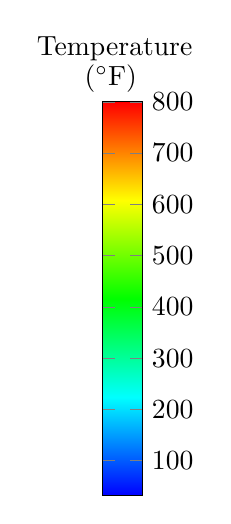
\begin{tikzpicture}
\node at (0.45,0.67) {Temperature};
\node at (0.4,0.3) {($^\circ$F)};
\begin{axis}[
    hide axis,
    scale only axis,
    height=0pt,
    width=0pt,
    colorbar,
    point meta min=32,
    point meta max=800,
    colorbar style={
        height=5cm,
        ytick={100,200,...,800}
    }]
    \addplot [draw=none] coordinates {(0,0)};
\end{axis}
\end{tikzpicture}
%\end{document}
\caption{FDS simulated temperature vectors, 2~s before (top) and 60~s after (bottom) first rear basement window failure (342~s).}
\label{fig:smv_temperature_vectors}
\end{figure}


\chapter{Discussion of Simulation Results}
\label{sec:discussion}

The results of the FDS simulations are discussed in the following two sections. The first section addresses the results of the simulation as they relate to the flow path and the conditions in the interior stairwell. The second section examines the model results and observed outcomes of the fire incident as they relate to tactics discussed in recent experimental research. 

\section{Simulated Interior Stairwell Flow Path}
\label{sec:simulated_flow_path}

The NIOSH report~\cite{NIOSH:Bowyer2} indicated that the interior stairwell on the front side of the structure was used to determine that the fire was located in the basement. From the simulation results (Section~\ref{sec:temperature}), the conditions in the interior stairwell were initially tenable. After the rear basement windows failed, the simulation results indicate a high-hazard area (temperatures greater than 260~$^{\circ}$C or 500~$^{\circ}$F) in the stairwell near the laundry room landing area.

After the rear basement windows failed, a flow path was established between the basement living room area and the doors located on the front side of the structure (the front door and the garage door). The rear basement window failures resulted in a rapid change in the conditions within the flow path. After the rear basement windows began to fail, the combustion gases at elevated temperature and pressure in the basement flowed upwards towards lower pressure areas via the stairwell. The two E26 firefighters were located in the flow path between the basement and the doors on the front side of the structure.

The arrows shown in Fig.~\ref{fig:flow_path_top} indicate the simulated flow direction of gases from the basement after the window failures. In this figure, the red arrows indicate elevated gas temperatures, and the blue arrows indicate relatively cooler gas temperatures. The arrow that transitions from red to blue indicates that the heated gases were cooling as they flowed away from the fire towards the front of the structure. The two arrows located at the door on the second floor (towards the front of the structure) indicate bi-directional flow. At that doorway, cool ambient air flowed towards the fire near the bottom of the door, and hot gases flowed away from the fire near the top of the door.

\begin{figure}[!ht]
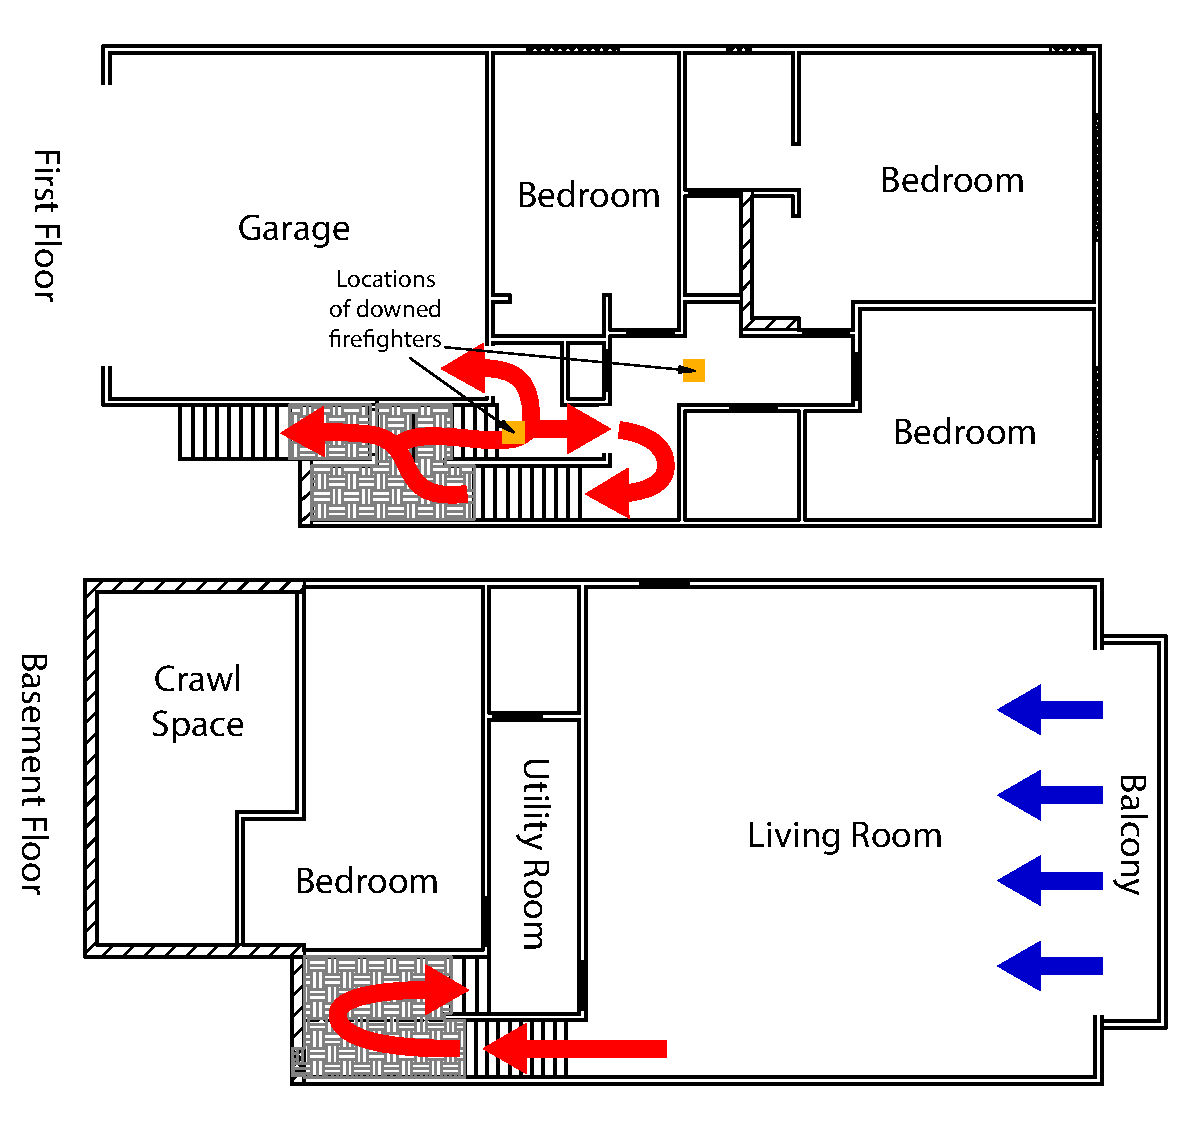
\includegraphics[width=5.0in]{../Figures/Flow_Path_Top}
\caption{Summary of simulated flow path in the stairwell on the basement floor and first floor after the rear basement window failures.}
\label{fig:flow_path_top}
\end{figure}

\section{Assessing the Hazard}
\label{sec:assessing_the_hazard}

A person is susceptible to second-degree burn injuries if exposed to temperatures greater than 55~$^{\circ}$C (130~$^{\circ}$F)~\cite{contactburn}. Although firefighters wear protective gear, gear only offers a finite amount of protection. The polycarbonate in a self contained breathing apparatus begins to soften when the material temperature reaches approximately 140~$^{\circ}$C (284~$^{\circ}$F)~\cite{mensch2011emergency}. Structural fire fighting coats and pants are tested to withstand temperatures of 260~$^{\circ}$C (500~$^{\circ}$F)~\cite{nfpa2013standard}. Prolonged exposure to elevated temperatures can result in a significant amount of heat transferred to the firefighter, putting him/her at risk. Exposure of equipment to temperatures of 260~$^{\circ}$C (500~$^{\circ}$F) represents a Class~III exposure~\cite{Donnelly2006}. Firefighters are at increased risk levels when encountering Class~III exposure conditions for more than 5~minutes~\cite{Donnelly2006}. Based on the simulation results shown in Section~\ref{sec:temperature}, the simulated flow path temperatures in the interior stairwell were in excess of 600~$^{\circ}$C (1100~$^{\circ}$F) and the flow velocities were approximately 9~m/s (20 mph).

% The temperature of the gases that flowed into the interior stairwell was estimated to be approximately XXX~$^{\circ}$C (XXX~$^{\circ}$F), which exceeds the Class~III exposure temperature of 260~$^{\circ}$C (500~$^{\circ}$F).

% Prior to the interior door failure, the elevated temperatures on the second floor were limited to the rear porch, as shown in Fig.~\ref{fig:temp_top_159}. The temperatures were greatest at the back-left corner where there is sufficient oxygen due to the section of porch wall that had burned away and allowed additional oxygen to mix with the fuel-rich fire gases. Five seconds after the interior door failed, hot gases traveled the length of the interior hallway and approached the doorway into the kitchen, which was approximately 4.5~m (14.8~ft) away from the source fire, as shown in Fig.~\ref{fig:temp_top_165}. Within 60~s of the interior door failure, the hallway temperatures were approximately at or above 260~$^{\circ}$C (500~$^{\circ}$F) throughout the hallway, as shown in Fig.~\ref{fig:temp_top_220}. These results indicate that the high temperature gases seen 5~s after failure were not just a burst but rather the front of a sustained exhaust gas flow from the fire burning in the enclosed rear porch. The conditions in this hallway changed from tenable to high-hazard very rapidly following the door failure. Figure~\ref{fig:temp_top_220} also shows that the temperatures in the kitchen were at or below 90~$^{\circ}$C (194~$^{\circ}$F), and the temperatures at the top of the stairs were at or below 70~$^{\circ}$C (158~$^{\circ}$F). At these locations within the structure, the exhaust gases in the flow path were cooled and diluted by the inflowing ambient gas. These simulated temperatures are consistent with the post-incident conditions that were documented in the kitchen and second floor stairwell.

% Insert top-down figures from SMV showing laundry room landing area temperatures.

% \begin{figure}[!ht]
% 
\includegraphics[width=6.5in]{../Figures/west_50th_baseline_top_159_6ft}
% %\documentclass{standalone}
%\usepackage{pgfplots}
%\begin{document}
%\pgfplotsset{
%	colormap={blackwhite}{[5pt]
%		rgb255(0pt)=(0,0,255); 
%		rgb255(100pt)=(0,255,255); 
%		rgb255(200pt)=(0,255,0); 
%		rgb255(300pt)=(255,255,0); 
%		rgb255(400pt)=(255,0,0)
%	},
%}
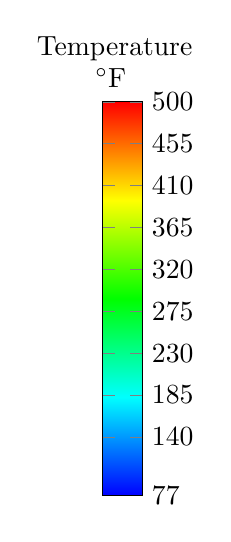
\begin{tikzpicture}
\node at (0.45,0.67) {Temperature};
\node at (0.4,0.3) {$^\circ$F};
\begin{axis}[
    hide axis,
    scale only axis,
    height=0pt,
    width=0pt,
    colorbar,
    point meta min=77,
    point meta max=500,
    colorbar style={
        height=5cm,
        ytick={77,140,185,...,500}
    }]
    \addplot [draw=none] coordinates {(0,0)};
\end{axis}
\end{tikzpicture}
%\end{document} 
% %\documentclass{standalone}
%\usepackage{pgfplots}
%\begin{document}
%\pgfplotsset{
%	colormap={blackwhite}{[5pt]
%		rgb255(0pt)=(0,0,255); 
%		rgb255(100pt)=(0,255,255); 
%		rgb255(200pt)=(0,255,0); 
%		rgb255(300pt)=(255,255,0); 
%		rgb255(400pt)=(255,0,0)
%	},
%}
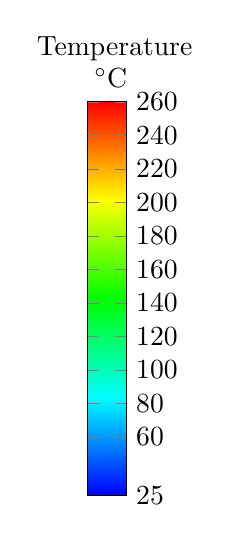
\begin{tikzpicture}
\node at (0.65,0.67) {Temperature};
\node at (0.6,0.3) {$^\circ$C};
\begin{axis}[
    hide axis,
    scale only axis,
    height=0pt,
    width=0pt,
    colorbar,
    point meta min=25,
    point meta max=260,
    colorbar style={
        height=5cm,
        ytick={25,60,80,...,260}
    }]
    \addplot [draw=none] coordinates {(0,0)};
\end{axis}
\end{tikzpicture}
%\end{document}

% \caption[Temperature contours on the second floor, 1~s prior to interior door failure.]
% {Temperature contours on the second floor, 1~s prior to interior door failure, 1.83~m (6~ft) above the floor.}
% \label{fig:temp_top_159}
% \end{figure}

% \begin{figure}[!ht]
% 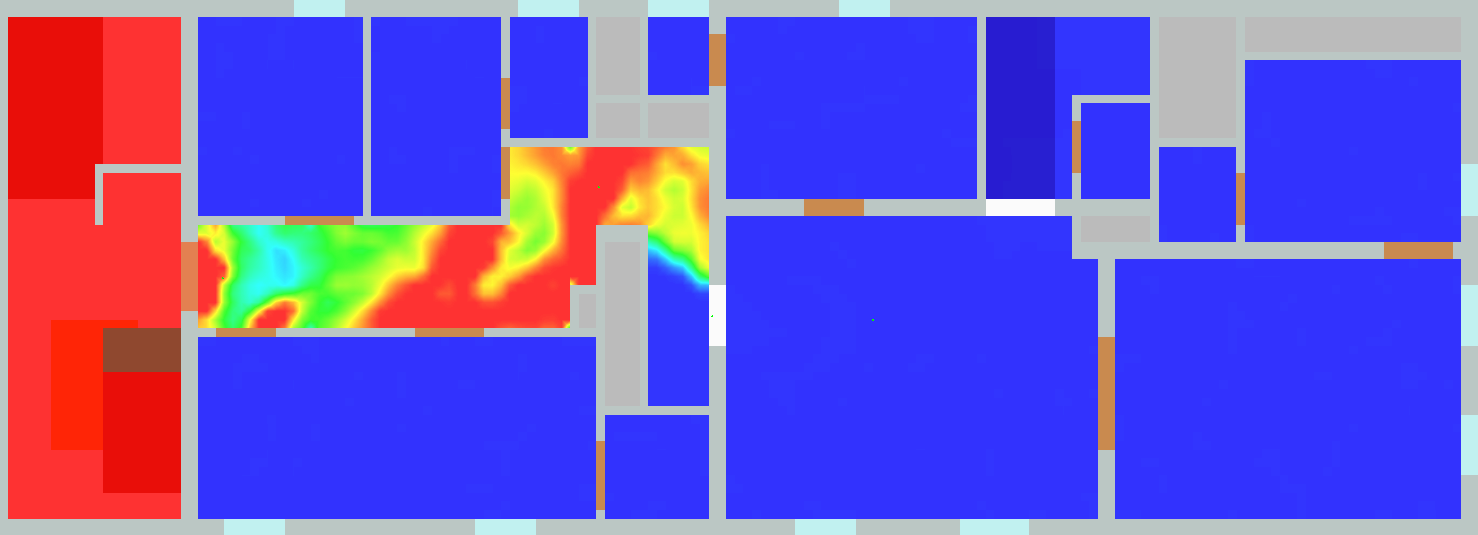
\includegraphics[width=6.5in]{../Figures/west_50th_baseline_top_165_6ft}
% %\documentclass{standalone}
%\usepackage{pgfplots}
%\begin{document}
%\pgfplotsset{
%	colormap={blackwhite}{[5pt]
%		rgb255(0pt)=(0,0,255); 
%		rgb255(100pt)=(0,255,255); 
%		rgb255(200pt)=(0,255,0); 
%		rgb255(300pt)=(255,255,0); 
%		rgb255(400pt)=(255,0,0)
%	},
%}
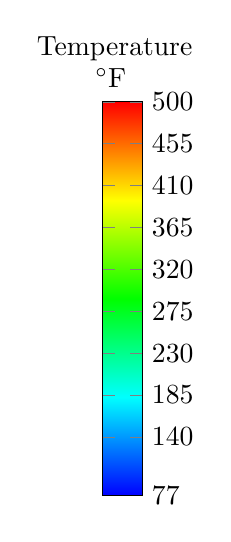
\begin{tikzpicture}
\node at (0.45,0.67) {Temperature};
\node at (0.4,0.3) {$^\circ$F};
\begin{axis}[
    hide axis,
    scale only axis,
    height=0pt,
    width=0pt,
    colorbar,
    point meta min=77,
    point meta max=500,
    colorbar style={
        height=5cm,
        ytick={77,140,185,...,500}
    }]
    \addplot [draw=none] coordinates {(0,0)};
\end{axis}
\end{tikzpicture}
%\end{document} 
% %\documentclass{standalone}
%\usepackage{pgfplots}
%\begin{document}
%\pgfplotsset{
%	colormap={blackwhite}{[5pt]
%		rgb255(0pt)=(0,0,255); 
%		rgb255(100pt)=(0,255,255); 
%		rgb255(200pt)=(0,255,0); 
%		rgb255(300pt)=(255,255,0); 
%		rgb255(400pt)=(255,0,0)
%	},
%}
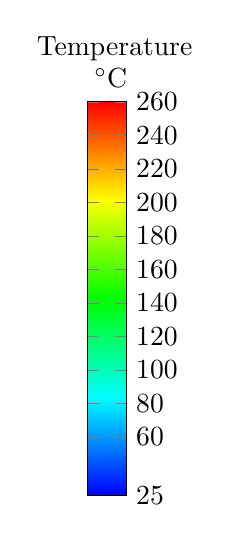
\begin{tikzpicture}
\node at (0.65,0.67) {Temperature};
\node at (0.6,0.3) {$^\circ$C};
\begin{axis}[
    hide axis,
    scale only axis,
    height=0pt,
    width=0pt,
    colorbar,
    point meta min=25,
    point meta max=260,
    colorbar style={
        height=5cm,
        ytick={25,60,80,...,260}
    }]
    \addplot [draw=none] coordinates {(0,0)};
\end{axis}
\end{tikzpicture}
%\end{document}

% \caption[Temperature contours on the second floor, 5~s after interior door failure.]
% {Temperature contours on the second floor, 5~s after interior door failure, 1.83~m (6~ft) above the floor.}
% \label{fig:temp_top_165}
% \end{figure}

% \begin{figure}[!ht]
% 
\includegraphics[width=6.5in]{../Figures/west_50th_baseline_top_220_6ft}
% %\documentclass{standalone}
%\usepackage{pgfplots}
%\begin{document}
%\pgfplotsset{
%	colormap={blackwhite}{[5pt]
%		rgb255(0pt)=(0,0,255); 
%		rgb255(100pt)=(0,255,255); 
%		rgb255(200pt)=(0,255,0); 
%		rgb255(300pt)=(255,255,0); 
%		rgb255(400pt)=(255,0,0)
%	},
%}
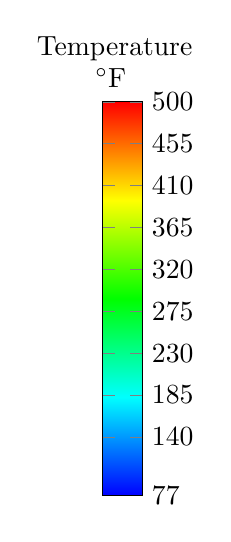
\begin{tikzpicture}
\node at (0.45,0.67) {Temperature};
\node at (0.4,0.3) {$^\circ$F};
\begin{axis}[
    hide axis,
    scale only axis,
    height=0pt,
    width=0pt,
    colorbar,
    point meta min=77,
    point meta max=500,
    colorbar style={
        height=5cm,
        ytick={77,140,185,...,500}
    }]
    \addplot [draw=none] coordinates {(0,0)};
\end{axis}
\end{tikzpicture}
%\end{document} 
% %\documentclass{standalone}
%\usepackage{pgfplots}
%\begin{document}
%\pgfplotsset{
%	colormap={blackwhite}{[5pt]
%		rgb255(0pt)=(0,0,255); 
%		rgb255(100pt)=(0,255,255); 
%		rgb255(200pt)=(0,255,0); 
%		rgb255(300pt)=(255,255,0); 
%		rgb255(400pt)=(255,0,0)
%	},
%}
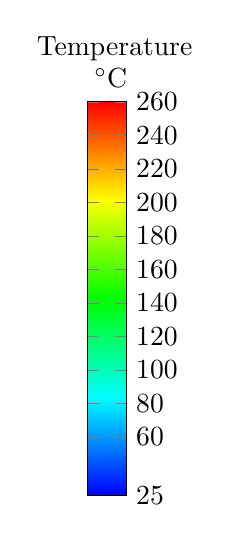
\begin{tikzpicture}
\node at (0.65,0.67) {Temperature};
\node at (0.6,0.3) {$^\circ$C};
\begin{axis}[
    hide axis,
    scale only axis,
    height=0pt,
    width=0pt,
    colorbar,
    point meta min=25,
    point meta max=260,
    colorbar style={
        height=5cm,
        ytick={25,60,80,...,260}
    }]
    \addplot [draw=none] coordinates {(0,0)};
\end{axis}
\end{tikzpicture}
%\end{document}

% \caption[Temperature contours on the second floor, 60~s after interior door failure.]
% {Temperature contours on the second floor, 60~s after interior door failure, 1.83~m (6~ft) above the floor.}
% \label{fig:temp_top_220}
% \end{figure}

\section{Tactical Considerations}
\label{sec:tactical_condsiderations}

In this fire incident, the failure of the basement windows on the rear side of the structure coincided with a rapid change in the thermal conditions in the interior stairwell. The rear basement window failures resulted in the establishment of a flow path within the interior stairwell with highly hazardous conditions. These conditions would be equivalent to or greater than a Class~III exposure~\cite{Donnelly2006}.

After the primary search was conducted, closing the interior doors (i.e., door control) could have inhibited the establishment of a flow path in the interior stairwell. A 360$^\circ$ scene size-up by the arriving firefighters could have helped determine the location of the fire in the basement and identify potential flow paths within the structure. The interior stairwell acted as a chimney for hot gases in the basement to flow towards areas of lower pressure via the interior stairwell towards the front of the structure. Firefighters should avoid placing themselves within a flow path, where elevated temperatures and flow velocities can present hazardous conditions and increase the rate of heat transfer to firefighting gear via convection.

The timing of the interior attack in the basement occurred after delays in forcible entry operations on the exterior basement door. Suppression operations should be coordinated with interior operations to reduce thermal hazards related to flow paths within a structure. Ongoing research by NIST, Underwriters Laboratories (UL), and others has demonstrates that applying water from the exterior into the fire area of a structure (prior to the start of interior operations) can significantly improve the safety of firefighters by reducing the thermal hazard from the fire and reducing the potential for developing high velocity hot gas flows within the structure~\cite{madrzykowski2009fire, kerber2009fire}.

There have been many previous fire incidents~\cite{NIOSH:Pettit,NIOSH:Washenitz,NIOSH:Mezzanotte,NIOSH:McFall,NIOSH:McFall2,NIOSH:McFall3,NIOSH:Berardinelli,NIOSH:Koedam,NIOSH:McFall4,NIOSH:Tarley,NIOSH:Braddee,NIOSH:Merinar,NIOSH:Bowyer2,NIOSH:Loflin,NIOSH:Bowyer} in which changes in the flow paths are thought to have had an adverse impact on firefighter and occupant safety. Table~\ref{tab:LODD} lists the NIOSH investigation reports from the past 15 years in which it could be determined that a flow path played a role in the related incident. This table lists the NIOSH investigation number, the outcome, and a brief description of the flow path details.

Based on a review of these incidents, it is clear that fires with rapidly developing or changing flow paths are a significant hazard to the fire service. The development of (or changes to) a flow path could be caused by the failure of a component of the structure, such as a door, window, or portion of a ceiling, wall or floor. Environmental conditions such as wind can generate hazardous thermal conditions within a flow path. Uncoordinated ventilation can also be the cause of increased thermal hazards within a flow path. 

\begin{table}[!ht]
\caption[Flow path related LODD/LODI incidents]{Flow path related LODD/LODI incidents}
\begin{tabular}{lll}
\toprule
NIOSH Report No. & No. of LODDs/LODIs & Flow Path Details                                            \\
\midrule
99-F01   \cite{NIOSH:Pettit}        &  3 LODDs            &  From apartment into hallway on 10th     \\
                                    &                     &  floor of high-rise apartment building   \\
99-F21   \cite{NIOSH:Washenitz}     &  2 LODDs            &  Basement to 1st floor                   \\
                                    &  2 LODIs            &                                          \\
F2000-04 \cite{NIOSH:Mezzanotte}    &  3 LODDs            &  1st floor to 2nd floor                  \\
                                    &  3 civilian deaths  &                                          \\
F2000-16 \cite{NIOSH:McFall}        &  1 LODD             &  2nd floor hallway through               \\
                                    &  1 LODI             &  2nd floor apartment                     \\
                                    &  1 civilian death   &                                          \\
F2000-23 \cite{NIOSH:McFall2}       &  1 LODD             &  From ground level to 1st floor then to  \\
                                    &  2 LODIs            &  2nd floor, flow exited through ceiling  \\
F2000-43 \cite{NIOSH:McFall3}       &  1 serious LODI     &  1st floor to 2nd floor                  \\
                                    &  2 other LODIs      &                                          \\
F2004-02 \cite{NIOSH:Berardinelli}  &  1 LODD             &  1st floor to basement                   \\
F2005-02 \cite{NIOSH:Koedam}        &  1 LODD             &  Rear to front of the building           \\
                                    &  4 LODIs            &                                          \\
F2005-04 \cite{NIOSH:McFall4}       &  1 LODD             &  Basement to 1st floor                   \\
                                    &  9 LODIs            &                                          \\
F2007-09 \cite{NIOSH:Tarley}        &  1 LODD             &  3 story training burn - flow through    \\
                                    &  2 LODIs            &  all levels                              \\
F2007-35 \cite{NIOSH:Braddee}       &  4 LODIs            &  1st floor to 2nd floor                  \\
F2009-11 \cite{NIOSH:Merinar}       &  2 LODDs            &  Rear to front of the building           \\
F2011-13 \cite{NIOSH:Bowyer2}       &  2 LODDs            &  Lower level up stairs and through       \\
                                    &                     &  entry door and garage                   \\
F2011-31 \cite{NIOSH:Loflin}        &  1 LODD             &  Fire extended from lower level apartme  \\
F2012-28 \cite{NIOSH:Bowyer}        &  1 LODD             &  Attic fire extended into closed         \\
                                    &  1 LODI             &  porch and then into 2nd floor           \\
\bottomrule
\end{tabular}
\label{tab:LODD}
\end{table}


\chapter{Summary}
\label{sec:summary}

NIST's Fire Dynamics Simulator was used to provide insight into the fire dynamics of a fire that occurred within a multi-level, single-family residential structure in San Francisco, CA, that resulted in the death of two firefighters. The fuel, fire size, and fire growth rate that were used in the FDS simulations were estimated by taking into account all of the available information including the NIOSH post-incident report~\cite{NIOSH:Bowyer2}, post-incident pictures, and relevant literature. This resulted in a maximum specified source fire of approximately 20~MW in the basement and rear balcony of the structure. Based on the limited ventilation conditions in the basement, the FDS simulation results indicated a HRR of approximately 2~MW as a result of the limited supply of oxygen. After the rear basement windows failed, the HRR increased to approximately 32~MW before it reached a steady-state value of approximately 20~MW.

The fire originated in the basement, and the interior stairwell acted as a chimney for hot gases in the basement to flow towards areas of lower pressure via the interior stairwell towards the front of the structure. After the rear basement windows failed, a flow path was established between the basement living room area and the doors located on the front side of the structure (the front door and the garage door). The rear basement window failures resulted in a rapid change in the conditions within the flow path. After the rear basement windows began to fail, the combustion gases at elevated temperature and pressure in the basement flowed upwards towards lower pressure areas via the stairwell. The temperature of the gases in the interior stairwell was estimated to be in excess of 600~$^{\circ}$C (1100~$^{\circ}$F), which exceeds the Class~III exposure temperature of 260~$^{\circ}$C (500~$^{\circ}$F).

Unfortunately, two E26 firefighters were located in the flow path between the basement and the doors on the front side of the structure. After a Mayday call, both firefighters were removed from the structure and immediate medical treatment was provided. The two firefighters were transported to the local medical center where the lieutenant was pronounced dead and the fire fighter/paramedic died two days later.


\chapter*{Acknowledgments}

The authors would like to thank XXXX. The authors would also like to thank John Culbertson of Central Valley Fire District, MT, for his assistance in compiling Table~\ref{tab:LODD}. Finally, the authors would also like to thank Keith Stakes of NIST and Joseph Willi of the University of Illinois Urbana-Champaign for their assistance in creating the drawings of the structure.

\bibliography{../../../Bibliography/FDS_refs,../../../Bibliography/FDS_general}

\appendix

\chapter{Dimensioned Drawings}
\label{sec:drawings}

\begin{figure}[!ht]
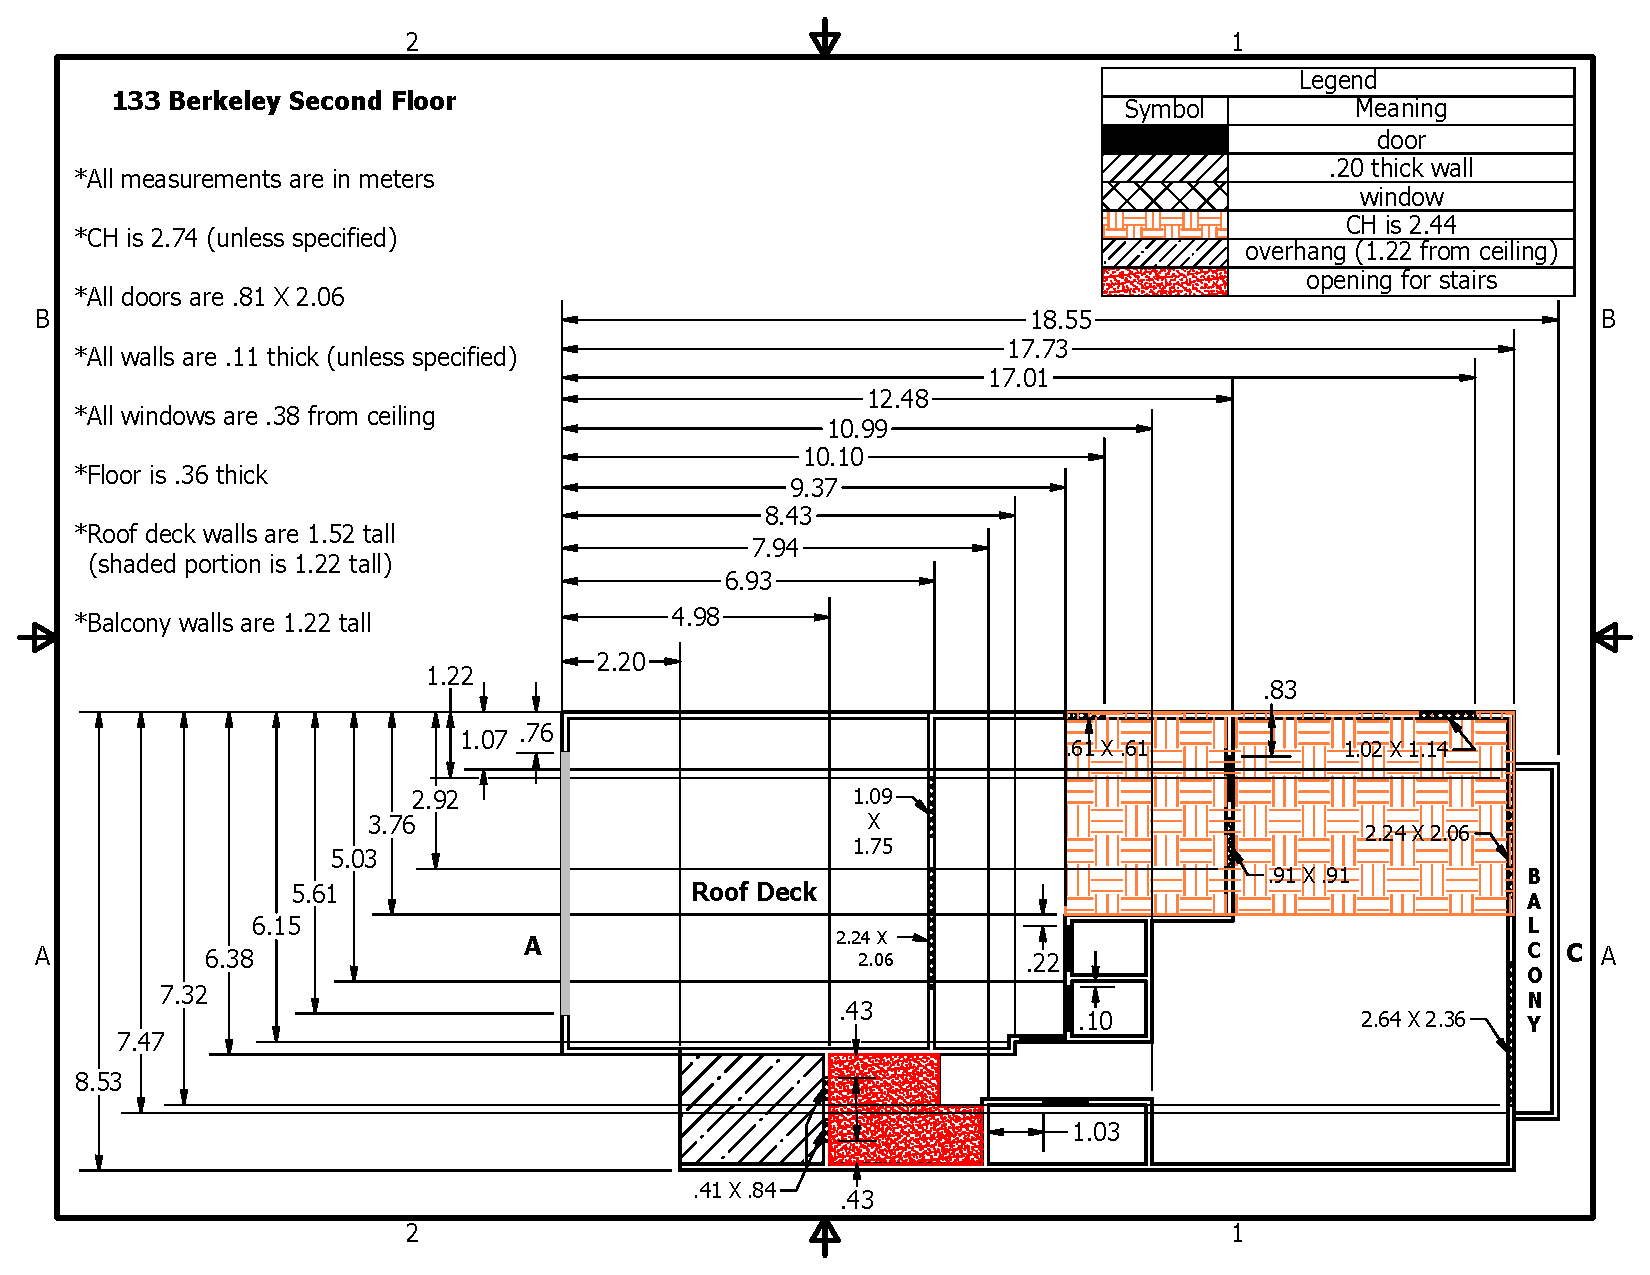
\includegraphics[width=6.5in]{../Figures/Drawing_Second_Floor_Metric}
\caption[Dimensioned drawing of the second floor.]{Dimensioned drawing of the second floor. The measurements are accurate to within 15~cm (6~in).}
\label{fig:drawing_second_floor}
\end{figure}

\begin{figure}[!ht]
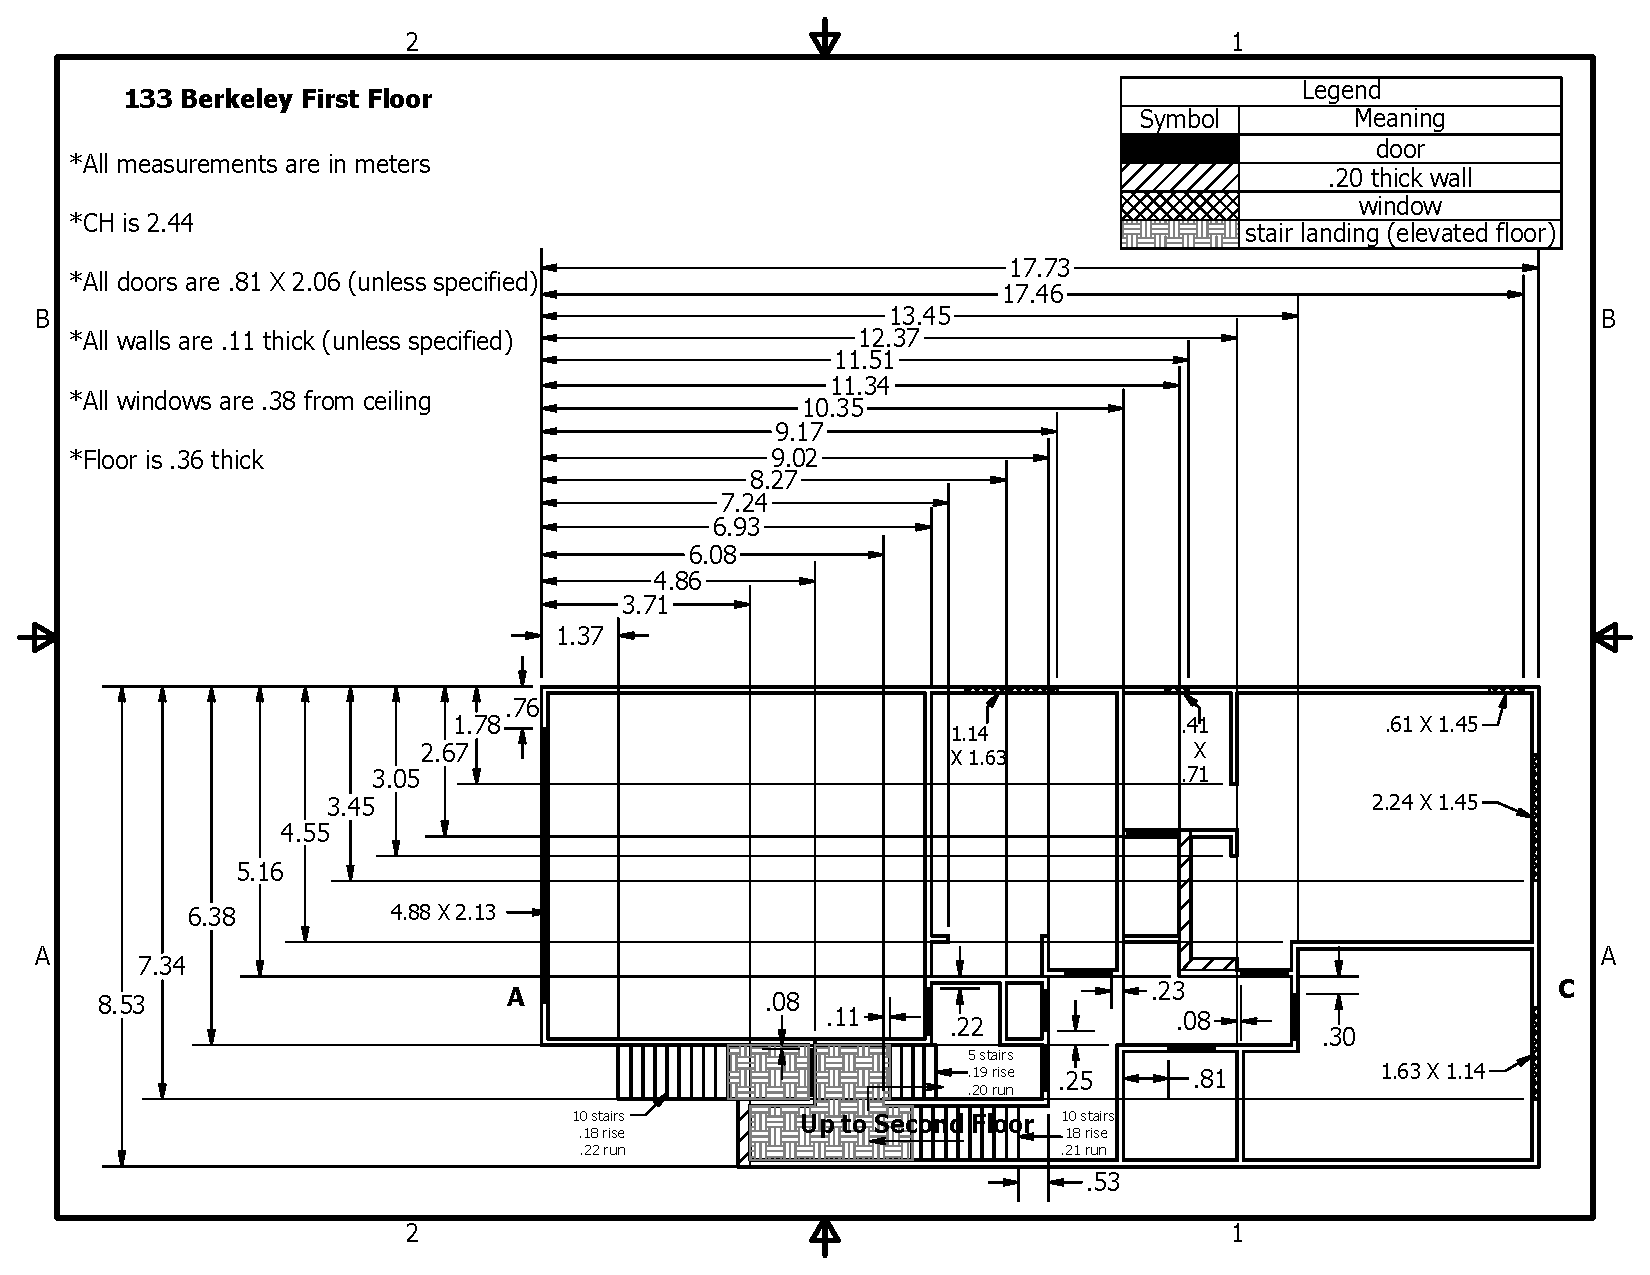
\includegraphics[width=6.5in]{../Figures/Drawing_First_Floor_Metric}
\caption[Dimensioned drawing of the first floor.]{Dimensioned drawing of the first floor. The measurements are accurate to within 15~cm (6~in).}
\label{fig:drawing_first_floor}
\end{figure}

\begin{figure}[!ht]
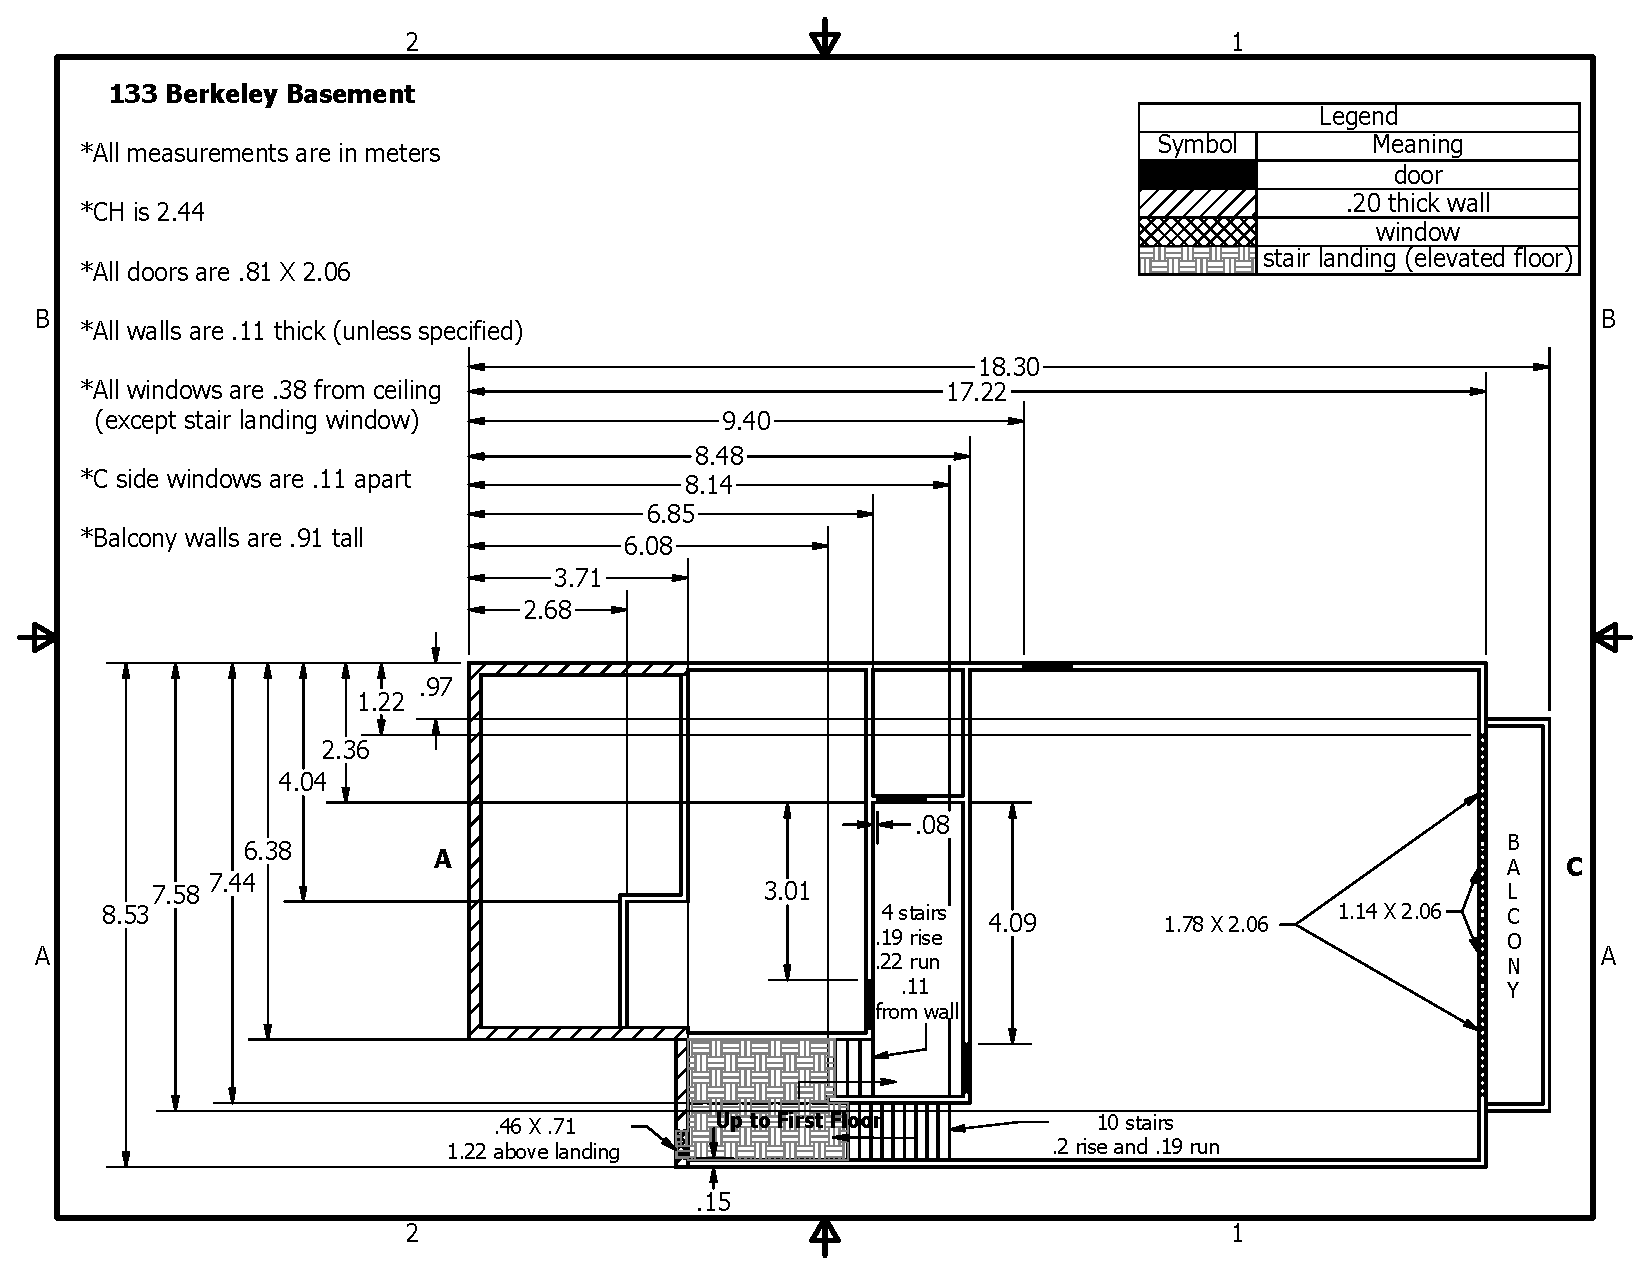
\includegraphics[width=6.5in]{../Figures/Drawing_Basement_Metric}
\caption[Dimensioned drawing of the basement.]{Dimensioned drawing of the basement. The measurements are accurate to within 15~cm (6~in).}
\label{fig:drawing_basement}
\end{figure}

\end{document}
